% This is the Reed College LaTeX thesis template. Most of the work
% for the document class was done by Sam Noble (SN), as well as this
% template. Later comments etc. by Ben Salzberg (BTS). Additional
% restructuring and APA support by Jess Youngberg (JY).
% Your comments and suggestions are more than welcome; please email
% them to cus@reed.edu
%
% See https://www.reed.edu/cis/help/LaTeX/index.html for help. There are a
% great bunch of help pages there, with notes on
% getting started, bibtex, etc. Go there and read it if you're not
% already familiar with LaTeX.
%
% Any line that starts with a percent symbol is a comment.
% They won't show up in the document, and are useful for notes
% to yourself and explaining commands.
% Commenting also removes a line from the document;
% very handy for troubleshooting problems. -BTS

% As far as I know, this follows the requirements laid out in
% the 2002-2003 Senior Handbook. Ask a librarian to check the
% document before binding. -SN

%%
%% Preamble
%%
% \documentclass{<something>} must begin each LaTeX document
\documentclass[12pt,oneside,a4paper]{reedthesis}
% Packages are extensions to the basic LaTeX functions. Whatever you
% want to typeset, there is probably a package out there for it.
% Chemistry (chemtex), screenplays, you name it.
% Check out CTAN to see: https://www.ctan.org/
%%
\usepackage{graphicx,latexsym}
\usepackage{amsmath}
\usepackage{amssymb,amsthm}
\usepackage{longtable,booktabs,setspace}
\usepackage{chemarr} %% Useful for one reaction arrow, useless if you're not a chem major
\usepackage[hyphens]{url}
% Added by CII
\usepackage[hidelinks]{hyperref}
\usepackage{lmodern}
\usepackage{float}
\floatplacement{figure}{tbp}
% Thanks, @Xyv
\usepackage{calc}
% End of CII addition
\usepackage{rotating}

% Next line commented out by CII
%%% \usepackage{natbib}
% Comment out the natbib line above and uncomment the following two lines to use the new
% biblatex-chicago style, for Chicago A. Also make some changes at the end where the
% bibliography is included.
%\usepackage{biblatex-chicago}
%\bibliography{thesis}
% \ifxetex
%   \usepackage{polyglossia}
%   \setmainlanguage{spanish}
%   % Tabla en lugar de cuadro
%   \gappto\captionsspanish{\renewcommand{\tablename}{Tabla}
%           \renewcommand{\listtablename}{Índice de tablas}}
% \else
%   \usepackage[spanish,es-tabla]{babel}
% \fi

% Added by CII (Thanks, Hadley!)
% Use ref for internal links
\renewcommand{\hyperref}[2][???]{\autoref{#1}}
\def\chapterautorefname{chapter}
\def\sectionautorefname{section}
\def\subsectionautorefname{subsection}
% End of CII addition

% Added by CII
\usepackage{caption}
\captionsetup{width=5in}
% End of CII addition

% \usepackage{times} % other fonts are available like times, bookman, charter, palatino

% Syntax highlighting #22

% To pass between YAML and LaTeX the dollar signs are added by CII
\title{Dinámica de la circulación zonalmente asimétrica del hemisferio sur}
\author{Lic. Elio Campitelli}
% The month and year that you submit your FINAL draft TO THE LIBRARY (May or December)
\date{BUENOS AIRES, 2023}
\division{Facultad de Ciencias Exactas y Naturales}
\advisor{Dra. Carolina Vera}
\institution{Universidad de Buenos Aires}
\degree{Tesis presentada para optar al título de Doctor de la Universidad de Buenos Aires en el Área de Ciencias de la Atmósfera y los Océanos}
%If you have two advisors for some reason, you can use the following
% Uncommented out by CII
\altadvisor{Dr.~Leandro Diaz}
\consejere{Dr.~Claudio Menendez}
\place{Centro de Investigaciones del Mar y la Atmósfera. CONICET-UBA}
% End of CII addition

%%% Remember to use the correct department!
\department{Departamento de Ciencias de la Atmósfera y los Océanos}
% if you're writing a thesis in an interdisciplinary major,
% uncomment the line below and change the text as appropriate.
% check the Senior Handbook if unsure.
%\thedivisionof{The Established Interdisciplinary Committee for}
% if you want the approval page to say "Approved for the Committee",
% uncomment the next line
%\approvedforthe{Committee}

% Added by CII
%%% Copied from knitr
%% maxwidth is the original width if it's less than linewidth
%% otherwise use linewidth (to make sure the graphics do not exceed the margin)
\makeatletter
\def\maxwidth{ %
  \ifdim\Gin@nat@width>\linewidth
    \linewidth
  \else
    \Gin@nat@width
  \fi
}
\makeatother

\makeatletter
\renewcommand{\@chapapp}{Capítulo}
\makeatother

% From {rticles}
\newlength{\csllabelwidth}
\setlength{\csllabelwidth}{3em}
\newlength{\cslhangindent}
\setlength{\cslhangindent}{1.5em}
% for Pandoc 2.8 to 2.10.1
\newenvironment{cslreferences}%
  {}%
  {\par}
% For Pandoc 2.11+
% As noted by @mirh [2] is needed instead of [3] for 2.12
\newenvironment{CSLReferences}[2] % #1 hanging-ident, #2 entry spacing
 {% don't indent paragraphs
  \setlength{\parindent}{0pt}
  % turn on hanging indent if param 1 is 1
  \ifodd #1 \everypar{\setlength{\hangindent}{\cslhangindent}}\ignorespaces\fi
  % set entry spacing
  \ifnum #2 > 0
  \setlength{\parskip}{#2\baselineskip}
  \fi
 }%
 {}
\usepackage{calc} % for calculating minipage widths
\newcommand{\CSLBlock}[1]{#1\hfill\break}
\newcommand{\CSLLeftMargin}[1]{\parbox[t]{\csllabelwidth}{#1}}
\newcommand{\CSLRightInline}[1]{\parbox[t]{\linewidth - \csllabelwidth}{#1}}
\newcommand{\CSLIndent}[1]{\hspace{\cslhangindent}#1}

\renewcommand{\contentsname}{Índice}
% End of CII addition

\setlength{\parskip}{0pt}

% Added by CII

\providecommand{\tightlist}{%
  \setlength{\itemsep}{0pt}\setlength{\parskip}{0pt}}

\Acknowledgements{
A mis directores, Carolina y Leandro, quienes luego de sufrirme durante una tesis de licenciatura, decidieron pasar otros 6 años guiando esta tesis de doctorado.
¡Prometo que esta es la última!

Al CONICET por darme de comer durante el doctorado, a la FCEN y el DCAO por ofrecer la educación de calidad que me permite investigar, y al CIMA por darme un lugar de trabajo y recursos para hacer lo que amo hacer.

A la comunidad de R, en cuyos amplios y cómodos hombros me paro para escribir esta tesis de forma abierta y reproducible.

A mi familia.
Clementina y David, cuyas contribuciones sentados sobre el teclado fueron imprescindibles.
Mis suegres, que me cebaron mate y compartieron bananas mientras escribía esta tésis.
Mi papá, que un día me sentó en una plaza de San Juan para hablarme de la gravitación.
Enrique, que me mostró la maleabilidad del plomo.
Goyo, que me ayudó a aprender a leer con la ``J'' de ``joder''.
Y mi mamá, con quién compartimos largas discusiones sobre cómo hacer ciencia y escribir papers; extraño no poder celebrar con ella con un brindis.

A Pao, la mejor compañera de trabajo y de vida.
}

\Dedication{

}

\Preface{

}

\Abstract{
\textbf{Dynamics of the Southern Hemisphere zonally asymmetric circulation}

This thesis' objective is to describe and improve our understanding of the zonally asymmetric circulation in the Southern Hemisphere in seasonal and longer timescales.
To that end, we used ERA5 data, Coupled Model Intercomparison Project Phase 6 (CMIP6) historical simulations and Detection and Attribution Model Intercomparison Project (DAMIP) sensibility experiments.
We computed the Complex Empirical Orthogonal Functions (cEOFs) of the 200 hPa and 50 hPa geopotental height zonal anomalies, which enabled us to characterise the amplitude and phase of the main variability patterns of the zonally asymmetric circulation.

Two main modes of variability were identified.
The first cEOF (cEOF1) represents the zonal wave 1 variability in the stratosphere and is associated with a Southern Annular mode (SAM) like pattern in the troposphere and significant stratospheric ozone anomalies.
Its 0º phase has a positive trend in the 1940--2020 period, consistent with the evolution of the ozone hole.
On the other hand, the second cEOF (cEOF2) represents a wave 3 pattern with maximum amplitude in the Pacific region mainly in the troposphere with a weaker signal in the stratosphere.
This mode is related to Pacific-South American mode (PSA) like spatial patterns and an SAM-like annular pattern.
Its impact on surface-level temperature and precipitation anomalies depends on its phase.
Although this mode is active in the absence of tropical forcing, tropical Pacific sea surface temperature anomalies do influence its phase.

We separated the SAM into its zonally symmetric (S-SAM) and asymmetric (A-SAM) parts.
The S-SAM is associated with an zonally symmetric annular pattern, whereas the A-SAM is associated with a zonal wave 3-4.
The correlation between El Niño-Southern Oscillation and SAM is due solely to the latter's asymmetric component, while the SAM index positive trend is only present in its symmetric component.
Regional impacts of each component are also distinct and correspond to distinct processes.

By studying the relationship between both SAM components and the main modes of variability we concluded that the cEOF1 is moderately related with the A-SAM, mainly in its 90º phase in the stratosphere.
The cEOF2 90º phase is highly correlated with the A-SAM in the troposphere, which indicates that these two indices are describing the same physical phenomenon.
This further suggest that the A-SAM might not be a physical mode and that it should be instead be understood as a phase of the cEOF2 (PSA) and it appears as part of the SAM due to the methods used to isolate it.

Finally, we studied these modes in CMIP6 historical simulations and found that they can represent them relatively well, although model ability varies widely.
The multimodel mean does represent them satisfactorily.
However, most models overestimate the relationship between these modes and sea surface temperatures.
Exploration of the external forcings which could explain the cEOF1 trend we found that the increase in greenhouse gasses forces a negative trend in the cEOF1 0º phase, while the change in stratospheric ozone forces a positive trend.
Both effects partially compensate to explain the almost null trend in the historical experiments.
For the 90º phase, both greenhouse gasses and stratospheric ozone force a negative trend, while stratospheric aerosols force a positive trend.
The balance of these forcings results a a negative trend.
}


\Resumen{
\textbf{Dinámica de la circulación zonalmente asimétrica del hemisferio sur}

El objetivo de esta tesis es describir y avanzar en el entendimiento de la circulación zonalmente asimétrica en el hemisferio sur en escalas estacionales y más largas.
Para ello, se utilizaron datos de reanálisis de ERA5, simulaciones históricas de del Proyecto de Intercomparación de Modelos Acoplados (CMIP6) y experimentos de sensibilidad del Proyecto de Intercomparación de Modelos de Detección y Atribución (DAMIP).
Se computaron las Funciones Empíricas Ortogonales Complejas (cEOF) de las anomalías zonales de altura geopotencial en 200 hPa y 50 hPa en conjunto, lo que permitió caracterizar los principales patrones de variabilidad de la circulación zonalmente asimétrica en fase y amplitud.

Se identificaron dos modos principales de variabilidad.
El primer cEOF (cEOF1) representa la variabilidad de la onda zonal 1 en la estratosfera y está asociado a un patrón de tipo Modo Anual del Sur (SAM) en la tropósfera y con anomalías significativas de ozono estratosférico.
Su fase de 0º presenta una tendencia positiva en el período 1940--2020 consistente con la evolución del agujero de la capa de ozono.
En cambio, el segundo cEOF (cEOF2) representa un patrón de onda 3 con magnitud máxima en el Pacífico en la tropósfera principalmente y con una señal menos significativa en la estratósfera.
Este modo está relacionado con patrones espaciales de tipo Patrón del Pacífico-Sudamérica (PSA) y con un patrón anular de tipo SAM.
Su impacto en las anomalías de temperatura del aire en superficie y de precipitación depende de su fase.
Si bien este modo está activo en ausencia de forzante tropical, las anomalías de temperatura de la superficie del mar en el Pacífico tropical determinan su fase.

Se realizó un estudio de la variabilidad del SAM separándola en su parte zonalmente simétrica (S-SAM) y asimétrica (A-SAM).
El S-SAM está asociado a un patrón anular zonalmente simétrico mientras que el A-SAM está asociado a un patrón de onda zonal 3-4.
La correlación entre el SAM y El Niño-Oscilación del Sur se debe únicamente a su parte asimétrica y la tendencia del SAM sólo se observa en su parte simétrica.
Los impactos regionales de cada componente también son diferentes y responden a distintos procesos.

El estudio de la relación de ambas componentes del SAM con los modos principales de variabilidad zonalmente asimétrica mostró que el cEOF1 está moderadamente relacionado con el A-SAM, principalmente su fase de 90º en la estratósfera.
La fase de 90º del cEOF2 está altamente correlacionada con el A-SAM en la tropósfera, lo que sugiere que se trata de dos índices que describen el mismo fenómeno.
Esto sugiere que el A-SAM no sea un modo físico sino que debe ser entendido como una fase del cEOF2 (PSA) y que sólo surge como parte del SAM debido a la metodología utilizada para aislarlo.

Finalmente, se analizaron estos modos en simulaciones históricas de CMIP6 y se encontró que la capacidad de los modelos de representar estos modos es relativamente buena aunque varía entre los modelos.
La media multi-modelo los representa de manera adecuada.
Asimismo se encontró que la mayoría de los modelos exageran la relación entre los modos y la temperatura de la superficie del mar.
En la exploración de la influencia de los forzantes externos en explicar las tendencias asociadas con las fases del cEOF1 se encontró que para la fase de 0º, el aumento de los gases de efecto invernadero fuerza una tendencia negativa, mientras que la variación del ozono estatosférico fuerza una tendencia positiva.
Ambas tendencias se compensan y la tendencia en los experimentos históricos es casi nula.
Para la fase de 90º, la variación tanto de los gases de efecto invernadero como del ozono estratosférico fuerzan una tendencia negativa, mientras que el forzante de los aerosoles estratosféricos fuerzan una tendencia positiva.
El balance de estos forzantes genera una tendencia negativa.
}

	\usepackage{setspace}\onehalfspacing
\usepackage[spanish,es-tabla]{babel}
\usepackage[colorinlistoftodos]{todonotes}
\usepackage{subfig}
	\usepackage{booktabs}
\usepackage{longtable}
\usepackage{array}
\usepackage{multirow}
\usepackage{wrapfig}
\usepackage{float}
\usepackage{colortbl}
\usepackage{pdflscape}
\usepackage{tabu}
\usepackage{threeparttable}
\usepackage{threeparttablex}
\usepackage[normalem]{ulem}
\usepackage{makecell}
\usepackage{xcolor}
% End of CII addition
%%
%% End Preamble
%%
%

\usepackage{newpxtext,newpxmath}
\usepackage[T1]{fontenc}

\let\ORIincludegraphics\includegraphics
\renewcommand{\includegraphics}{%
  \write\listofgraphics{\thepage}%
  \ORIincludegraphics
}
\newwrite\listofgraphics
\AtBeginDocument{\immediate\openout\listofgraphics=\jobname.lis }
\AtEndDocument{\closeout\listofgraphics}

\begin{document}

% Everything below added by CII
  \maketitle

\frontmatter % this stuff will be roman-numbered
\pagestyle{empty} % this removes page numbers from the frontmatter


  \begin{resumen}
    \textbf{Dinámica de la circulación zonalmente asimétrica del hemisferio sur}

    El objetivo de esta tesis es describir y avanzar en el entendimiento de la circulación zonalmente asimétrica en el hemisferio sur en escalas estacionales y más largas.
    Para ello, se utilizaron datos de reanálisis de ERA5, simulaciones históricas de del Proyecto de Intercomparación de Modelos Acoplados (CMIP6) y experimentos de sensibilidad del Proyecto de Intercomparación de Modelos de Detección y Atribución (DAMIP).
    Se computaron las Funciones Empíricas Ortogonales Complejas (cEOF) de las anomalías zonales de altura geopotencial en 200 hPa y 50 hPa en conjunto, lo que permitió caracterizar los principales patrones de variabilidad de la circulación zonalmente asimétrica en fase y amplitud.

    Se identificaron dos modos principales de variabilidad.
    El primer cEOF (cEOF1) representa la variabilidad de la onda zonal 1 en la estratosfera y está asociado a un patrón de tipo Modo Anual del Sur (SAM) en la tropósfera y con anomalías significativas de ozono estratosférico.
    Su fase de 0º presenta una tendencia positiva en el período 1940--2020 consistente con la evolución del agujero de la capa de ozono.
    En cambio, el segundo cEOF (cEOF2) representa un patrón de onda 3 con magnitud máxima en el Pacífico en la tropósfera principalmente y con una señal menos significativa en la estratósfera.
    Este modo está relacionado con patrones espaciales de tipo Patrón del Pacífico-Sudamérica (PSA) y con un patrón anular de tipo SAM.
    Su impacto en las anomalías de temperatura del aire en superficie y de precipitación depende de su fase.
    Si bien este modo está activo en ausencia de forzante tropical, las anomalías de temperatura de la superficie del mar en el Pacífico tropical determinan su fase.

    Se realizó un estudio de la variabilidad del SAM separándola en su parte zonalmente simétrica (S-SAM) y asimétrica (A-SAM).
    El S-SAM está asociado a un patrón anular zonalmente simétrico mientras que el A-SAM está asociado a un patrón de onda zonal 3-4.
    La correlación entre el SAM y El Niño-Oscilación del Sur se debe únicamente a su parte asimétrica y la tendencia del SAM sólo se observa en su parte simétrica.
    Los impactos regionales de cada componente también son diferentes y responden a distintos procesos.

    El estudio de la relación de ambas componentes del SAM con los modos principales de variabilidad zonalmente asimétrica mostró que el cEOF1 está moderadamente relacionado con el A-SAM, principalmente su fase de 90º en la estratósfera.
    La fase de 90º del cEOF2 está altamente correlacionada con el A-SAM en la tropósfera, lo que sugiere que se trata de dos índices que describen el mismo fenómeno.
    Esto sugiere que el A-SAM no sea un modo físico sino que debe ser entendido como una fase del cEOF2 (PSA) y que sólo surge como parte del SAM debido a la metodología utilizada para aislarlo.

    Finalmente, se analizaron estos modos en simulaciones históricas de CMIP6 y se encontró que la capacidad de los modelos de representar estos modos es relativamente buena aunque varía entre los modelos.
    La media multi-modelo los representa de manera adecuada.
    Asimismo se encontró que la mayoría de los modelos exageran la relación entre los modos y la temperatura de la superficie del mar.
    En la exploración de la influencia de los forzantes externos en explicar las tendencias asociadas con las fases del cEOF1 se encontró que para la fase de 0º, el aumento de los gases de efecto invernadero fuerza una tendencia negativa, mientras que la variación del ozono estatosférico fuerza una tendencia positiva.
    Ambas tendencias se compensan y la tendencia en los experimentos históricos es casi nula.
    Para la fase de 90º, la variación tanto de los gases de efecto invernadero como del ozono estratosférico fuerzan una tendencia negativa, mientras que el forzante de los aerosoles estratosféricos fuerzan una tendencia positiva.
    El balance de estos forzantes genera una tendencia negativa.
  \end{resumen}


  \begin{abstract}
    \textbf{Dynamics of the Southern Hemisphere zonally asymmetric circulation}

    This thesis' objective is to describe and improve our understanding of the zonally asymmetric circulation in the Southern Hemisphere in seasonal and longer timescales.
    To that end, we used ERA5 data, Coupled Model Intercomparison Project Phase 6 (CMIP6) historical simulations and Detection and Attribution Model Intercomparison Project (DAMIP) sensibility experiments.
    We computed the Complex Empirical Orthogonal Functions (cEOFs) of the 200 hPa and 50 hPa geopotental height zonal anomalies, which enabled us to characterise the amplitude and phase of the main variability patterns of the zonally asymmetric circulation.

    Two main modes of variability were identified.
    The first cEOF (cEOF1) represents the zonal wave 1 variability in the stratosphere and is associated with a Southern Annular mode (SAM) like pattern in the troposphere and significant stratospheric ozone anomalies.
    Its 0º phase has a positive trend in the 1940--2020 period, consistent with the evolution of the ozone hole.
    On the other hand, the second cEOF (cEOF2) represents a wave 3 pattern with maximum amplitude in the Pacific region mainly in the troposphere with a weaker signal in the stratosphere.
    This mode is related to Pacific-South American mode (PSA) like spatial patterns and an SAM-like annular pattern.
    Its impact on surface-level temperature and precipitation anomalies depends on its phase.
    Although this mode is active in the absence of tropical forcing, tropical Pacific sea surface temperature anomalies do influence its phase.

    We separated the SAM into its zonally symmetric (S-SAM) and asymmetric (A-SAM) parts.
    The S-SAM is associated with an zonally symmetric annular pattern, whereas the A-SAM is associated with a zonal wave 3-4.
    The correlation between El Niño-Southern Oscillation and SAM is due solely to the latter's asymmetric component, while the SAM index positive trend is only present in its symmetric component.
    Regional impacts of each component are also distinct and correspond to distinct processes.

    By studying the relationship between both SAM components and the main modes of variability we concluded that the cEOF1 is moderately related with the A-SAM, mainly in its 90º phase in the stratosphere.
    The cEOF2 90º phase is highly correlated with the A-SAM in the troposphere, which indicates that these two indices are describing the same physical phenomenon.
    This further suggest that the A-SAM might not be a physical mode and that it should be instead be understood as a phase of the cEOF2 (PSA) and it appears as part of the SAM due to the methods used to isolate it.

    Finally, we studied these modes in CMIP6 historical simulations and found that they can represent them relatively well, although model ability varies widely.
    The multimodel mean does represent them satisfactorily.
    However, most models overestimate the relationship between these modes and sea surface temperatures.
    Exploration of the external forcings which could explain the cEOF1 trend we found that the increase in greenhouse gasses forces a negative trend in the cEOF1 0º phase, while the change in stratospheric ozone forces a positive trend.
    Both effects partially compensate to explain the almost null trend in the historical experiments.
    For the 90º phase, both greenhouse gasses and stratospheric ozone force a negative trend, while stratospheric aerosols force a positive trend.
    The balance of these forcings results a a negative trend.
  \end{abstract}



  \begin{acknowledgements}
    A mis directores, Carolina y Leandro, quienes luego de sufrirme durante una tesis de licenciatura, decidieron pasar otros 6 años guiando esta tesis de doctorado.
    ¡Prometo que esta es la última!

    Al CONICET por darme de comer durante el doctorado, a la FCEN y el DCAO por ofrecer la educación de calidad que me permite investigar, y al CIMA por darme un lugar de trabajo y recursos para hacer lo que amo hacer.

    A la comunidad de R, en cuyos amplios y cómodos hombros me paro para escribir esta tesis de forma abierta y reproducible.

    A mi familia.
    Clementina y David, cuyas contribuciones sentados sobre el teclado fueron imprescindibles.
    Mis suegres, que me cebaron mate y compartieron bananas mientras escribía esta tésis.
    Mi papá, que un día me sentó en una plaza de San Juan para hablarme de la gravitación.
    Enrique, que me mostró la maleabilidad del plomo.
    Goyo, que me ayudó a aprender a leer con la ``J'' de ``joder''.
    Y mi mamá, con quién compartimos largas discusiones sobre cómo hacer ciencia y escribir papers; extraño no poder celebrar con ella con un brindis.

    A Pao, la mejor compañera de trabajo y de vida.
  \end{acknowledgements}


  \hypersetup{linkcolor=black}
  \setcounter{secnumdepth}{2}
  \setcounter{tocdepth}{2}
  \tableofcontents

  \listoftables

  \listoffigures


\mainmatter % here the regular arabic numbering starts
\pagestyle{fancyplain} % turns page numbering back on

\hypertarget{intro}{%
\chapter{Introducción}\label{intro}}

La circulación general del hemisferio sur es más zonalmente simétrica que la del hemisferio norte, pero las anomalías zonales de la circulación tienen impactos regionales importantes en este hemisferio (p.ej. \protect\hyperlink{ref-hoskins2005}{Hoskins and Hodges, 2005}).
Las anomalías zonales modulan fuertemente los sistemas meteorológicos y el clima regional al influenciar el transporte meridional de calor, humedad y momento (\protect\hyperlink{ref-raphael2007}{M. N. Raphael, 2007}; \protect\hyperlink{ref-trenberth1980a}{K. E. Trenberth, 1980}) e incluso están relacionadas con la ocurrencia de extremos climáticos de alto impacto (\protect\hyperlink{ref-pezza2012}{Pezza et al., 2012}).

A pesar de estos impactos, las anomalías zonales de circulación han sido poco estudiadas en el hemisferio sur.
Por ejemplo, el principal patrón de circulación en latitudes medias -- el Modo Anular del Sur (SAM, por sus siglas en inglés) -- es entendido como un patrón zonalmente simétrico (\protect\hyperlink{ref-fogt2020}{Fogt and Marshall, 2020}) a pesar de estar asociado a significativas anomalías zonales de altura geopotencial.
Estas asimetrías zonales no han sido estudiadas extensivamente, pero en trabajos previos se ha sugerido que tienen un rol importante en modular los impactos regionales del SAM (\protect\hyperlink{ref-fan2007}{Fan, 2007}; \protect\hyperlink{ref-fogt2012}{Fogt et al., 2012}; \protect\hyperlink{ref-rosso2018}{Rosso et al., 2018}; \protect\hyperlink{ref-silvestri2009}{Silvestri and Vera, 2009}).

La circulación zonalmente asimétrica suele describirse en base a la amplitud y la fase de las ondas zonales obtenidas por la descomposición de Fourier de la altura geopotencial o de la presión a nivel del mar en cada latitud (\protect\hyperlink{ref-trenberth1980a}{K. E. Trenberth, 1980}; \protect\hyperlink{ref-turner2017}{Turner et al., 2017}; p.ej., \protect\hyperlink{ref-vanloon1972}{van Loon and Jenne, 1972}).
Bajo este enfoque, las ondas zonales 1 y 3 explican casi el 99\% de la varianza total del campo medio anual de las anomalías zonales de altura geopotencial de 500 hPa en 50ºS (\protect\hyperlink{ref-vanloon1972}{van Loon and Jenne, 1972}).
K. F. Trenberth and Mo (\protect\hyperlink{ref-trenberth1985}{1985}) concluyeron que la onda 3 tiene un rol importante en el desarrollo de los fenómenos de bloqueo.
Además, otros trabajos previos identificaron patrones de onda con números de onda dominantes 3-4 en latitudes extratropicales y subpolares con impactos regionales distintivos, como en las anomalías en la concentración de hielo marino antártico (\protect\hyperlink{ref-raphael2007}{M. N. Raphael, 2007}).

Con el propósito de identificar los factores importantes en el mantenimiento de la onda zonal 1 climatológica, Quintanar and Mechoso (\protect\hyperlink{ref-quintanar1995a}{1995}) realizaron un conjunto de experimentos de sensibilidad.
Encontró que ni la temperatura ni la orografía de la Antártida eran suficientes para explicar la amplitud de esta onda en latitudes subpolares, por lo que concluyó que los forzantes remotos debían jugar un papel importante.
Sin embargo, Watterson and James (\protect\hyperlink{ref-watterson1992}{1992}) y más recientemente Goyal et al. (\protect\hyperlink{ref-goyal2021a}{2021}) sugieren que la orografía antártica sí genera una onda 1 significativa.
Por otro lado Wang et al. (\protect\hyperlink{ref-wang2013}{2013}) encontraron que la destrucción y recuperación de la capa de ozono por forzantes antropogénicos está asociada a un aumento y disminución de la actividad de las ondas planetarias, respectivamente, pero su análisis no distingue cómo se modifican los distintos números de onda.

En cuanto a la onda zonal 3, Campitelli (\protect\hyperlink{ref-campitelli2018b}{2018}) realizó un estudio de sus propiedades y climatología.
Encontró que la onda zonal 3 mensual alcanza su máximo de amplitud entre 200 y 300 hPa y en 50ºS.
Además, la fase de esta onda zonal tiene un ciclo anual de aproximadamente 30º entre enero y junio, en coincidencia con lo observado por Mo and White (\protect\hyperlink{ref-mo1985}{1985}).
Excepto en noviembre y diciembre, la fase varía poco año a año con respecto a la fase media mensual, lo cual explica su relevancia en el campo medio.
En estos dos meses, en cambio, su fase es tan variable que no es posible hablar de una onda zonal 3 climatológica.

Experimentos de sensibilidad sugieren que los forzantes tropicales no son importantes para determinar la amplitud de la onda 3, sino que ayudan a fijarla en una fase preferencial y así se vea reflejada en el campo medio.
Para mostrar esto Campitelli (\protect\hyperlink{ref-campitelli2018b}{2018}) realizó simulaciones con el modelo SPEEDY eliminando la variabilidad de la temperatura de la superficie del mar (TSM) tropical, encontrando que la amplitud de la onda 3 era similar a la simulación control, pero que su fase era mucho más variable.
Estas conclusiones son consistentes con Goyal et al. (\protect\hyperlink{ref-goyal2021a}{2021}) quien realizó simulaciones con \emph{aquaplanet} al que le agregó los continentes individualmente, sugiriendo que la distribución de los tres continentes del hemisferio sur no tiene un rol relevante en el establecimiento de la onda 3 ni su importancia en el campo medio.
Este último trabajo además propone que la onda 3 representa un tren de onda con propagación meridional y amplitud relativamente localizada en vez de una onda planetaria con amplitud constante en todo el hemisferio.

Si la onda 3 es mejor entendida en término de trenes de onda con propagación meridional, el uso de la descomposición de Fourier no es válido, ya que ésta asume que la circulación puede describirse aproximadamente en términos de ondas zonales de amplitud constante a lo largo de un círculo de latitud.
Para abordar esta limitación, la técnica de Fourier puede generalizarse para integrar toda la amplitud de las ondas planetarias, independientemente del número de onda, calculando la envolvente de la onda (\protect\hyperlink{ref-irving2015}{Irving and Simmonds, 2015}).
La envolvente de onda puede representar ondas planetarias con diferente amplitud en diferentes longitudes, pero carece de información sobre la fase y el número de onda.
Utilizando este método, Irving and Simmonds (\protect\hyperlink{ref-irving2015}{2015}) demostró que la amplitud de las ondas planetarias en general está asociada a anomalías de concentración de hielo marino antártico y temperatura, así como a las anomalías de precipitación en regiones de topografía significativa en latitudes medias del hemisferio sur y en la Antártida.

Otro enfoque ampliamente utilizado para caracterizar las anomalías de la circulación troposférica del hemisferio sur es el cálculo de las Funciones Ortogonales Empíricas (EOF, también conocidas como Análisis de Componentes Principales).
El SAM aparece como el EOF que explica la mayor parte de la varianza de la circulación del hemisferio sur (\protect\hyperlink{ref-fogt2020}{Fogt and Marshall, 2020}), seguido por los EOF 2 y 3, normalmente conocidos como PSA1 y PSA2 (Patrón del Pacífico-Sudamérica), respectivamente.
Éstos describen trenes de ondas con propagación meridional que se originan en el Pacífico ecuatorial oriental y en el sector australiano-océano Índico, y viajan hacia el Atlántico Sur siguiendo un arco a lo largo de la costa antártica (\protect\hyperlink{ref-mo2001}{Mo and Paegle, 2001}).
Estos patrones influyen en las anomalías de precipitación en Sudamérica (\protect\hyperlink{ref-mo2001}{Mo and Paegle, 2001}).
Aunque estos patrones suelen derivarse aplicando EOF a anomalías temporales, M. Raphael (\protect\hyperlink{ref-raphael2003}{2003}) también aplicó métodos EOF específicamente a anomalías zonales.
Irving and Simmonds (\protect\hyperlink{ref-irving2016}{2016}) propuso una metodología novedosa para identificar objetivamente el patrón PSA utilizando la descomposición de Fourier.
Más recientemente Goyal et al. (\protect\hyperlink{ref-goyal2022}{2022}) creó un índice de amplitud y fase de la variabilidad zonal tipo onda 3 combinando los dos EOF principales de las anomalías del viento meridional.

Los patrones resultantes del análisis EOF son más flexibles que los modos derivados de la descomposición de Fourier, ya que pueden captar patrones de oscilación que no pueden caracterizarse por ondas puramente sinusoidales con amplitud constante.
No obstante, se limitan a los modos de oscilación estacionarios y no pueden representar correctamente la propagación meridional o la variación espacial de amplitud y fase.
Un único EOF también puede representar una mezcla de dos o más modos físicos.

Una tercera metodología comúnmente utilizada para describir anomalías de circulación consiste en identificar características particulares de interés y crear índices utilizando métodos simples como promedios y diferencias.
Ejemplos de esta metodología son el índice SAM de Gong and Wang (\protect\hyperlink{ref-gong1999}{1999}), el índice de actividad de la onda 3 hemisferio sur definido por M. N. Raphael (\protect\hyperlink{ref-raphael2004}{2004}) y el índice de circulación zonalmente asimétrica del hemisferio sur de Hobbs and Raphael (\protect\hyperlink{ref-hobbs2010}{2010}).
Estos métodos derivados se fundamentan en otras técnicas, como la descomposición de Fourier o las EOF, para identificar los centros de acción de los fenómenos descritos y pueden ser útiles para caracterizar rasgos que no se aprecian fácilmente mediante las mismas.
Este tipo de índices suelen ser fáciles de calcular, pero no suelen captar patrones no estacionarios.

En conclusión, las metodologías usadas en la literatura para estudiar la circulación atmosférica de gran escala no son apropiadas para el estudio de la onda 3, la cual es un patrón ondulatorio no estacionario con propagación meridional y amplitud no constante a lo largo de un círculo de latitud.

Una metodología alternativa que se ha propuesto para estudiar las ondas propagantes y estacionarias son las funciones ortogonales empíricas complejas (cEOF, \protect\hyperlink{ref-horel1984}{Horel, 1984}).
Este método amplía el análisis EOF para capturar oscilaciones con amplitud y fase variables y se ha aplicado al dominio temporal.
Por ejemplo, Krokhin and Luxemburg (\protect\hyperlink{ref-krokhin2007}{2007}) aplicó cEOF a las anomalías mensuales de precipitación basadas en estaciones y a las anomalías mensuales de temperatura en la región de Siberia Oriental y Extremo Oriente, lo cual permitió evaluar las características de propagación del principal patrón de cada variable.
Del mismo modo, Gelbrecht et al. (\protect\hyperlink{ref-gelbrecht2018}{2018}) aplicó cEOF a la precipitación diaria en Sudamérica, lo cual permitió caracterizar las características de propagación del dipolo de anomalías de precipitación observado entre el Sur de Sudamérica (SESA) y la Zona de Convergencia del Atlántico Sur.
Hasta donde se sabe, el análisis cEOF no se ha aplicado en el dominio espacial para capturar la naturaleza variable en fase de las ondas planetarias en la atmósfera.

El objetivo de esta tesis es entonces mejorar la descripción y comprensión de las asimetrías zonales de la circulación extratropical del hemisferio sur a través de:

\begin{enumerate}
\def\labelenumi{\arabic{enumi}.}
\item
  La identificación de los patrones principales de variabilidad de las asimetrías zonales identificándolas con el método de cEOF, porque permite considerar ondas planetarias de fase variable con amplitud variable.
  Se pone especial atención en el patrón de onda 1 y onda 3 por el conocimiento previo de su importante influencia tanto en la circulación extratropical del hemisferio sur como en el clima de sus continentes.
\item
  La exploración de las condiciones dinámicas estratosféricas, troposféricas y de superficie que explican la actividad de los patrones principales identificados en 1.
\item
  La exploración de las características simétricas y asimétricas del SAM a través de metodologías innovadoras, teniendo en cuenta que es el primer patrón de variabilidad temporal de la circulación extratropical del hemisferio sur.
\item
  La evaluación de la capacidad actual de los modelos climáticos como el CMIP6 para describir estos patrones principales de variabilidad.
\end{enumerate}

\hypertarget{onda3}{%
\chapter{Exploración de las formas de descripción de la onda 3}\label{onda3}}

En el \protect\hyperlink{intro}{capítulo anterior} se introdujeron conceptualmente algunos aspectos problemáticos de las metodologías e índices normalmente utilizados en la literatura para estudiar la circulación zonalmente asimétrica en el hemisferio sur.
Este capítulo realiza una primera evaluación de la descripción de la onda zonal 3 a través del del índice propuesto por M. N. Raphael (\protect\hyperlink{ref-raphael2004}{2004}) y de la descomposición de Fourier.

\hypertarget{muxe9todos}{%
\section{Métodos}\label{muxe9todos}}

\hypertarget{datos}{%
\subsection{Datos}\label{datos}}

Se utilizaron datos mensuales de altura geopotencial, del European Centre for Medium-Range Weather Forecasts Reanalysis versión 5 (ERA5) (\protect\hyperlink{ref-hersbach2020}{Hersbach et al., 2020}) a una resolución espacial de 2,5° de longitud por 2,5° de latitud.
Se utilizaron datos del período post-satelital (1979--2020) para garantizar la mayor cobertura posible de datos en el hemisferio sur que hayan alimentado al sistema de reanálisis.

\hypertarget{uxedndice-r04}{%
\subsection{Índice R04}\label{uxedndice-r04}}

El índice definido por M. N. Raphael (\protect\hyperlink{ref-raphael2004}{2004}) (de acá en adelante denominado ``R04'') se basa en un índice similar definido por Mo and White (\protect\hyperlink{ref-mo1985}{1985}) y es el índice más utilizado en la literatura para cuantificar la actividad de la onda zonal 3 del hemisferio sur.
Se calcula como el promedio de las anomalías zonales estandarizadas del promedio móvil de tres meses de altura geopotencial en 49ºS y en 500 hPa en tres ubicaciones elegidas para coincidir aproximadamente con los máximos climatológicos de la onda 3 según van Loon and Jenne (\protect\hyperlink{ref-vanloon1972}{1972}): 50ºE, 166ºE y 76ºO.
Valores positivos y negativos indican, por lo tanto, anomalías positivas y negativas~ alrededor de estas ubicaciones, respectivamente.
El promedio móvil de tres meses se aplica para evitar que el índice sea sensible al ciclo estacional de la localización de la onda 3 climatológica.
Dado que se utilizaron datos de reanálisis con una resolución de 2,5º, se calculó el índice con los puntos más cercanos: 50°E, 165°E, y 75°O en 50°S.

\hypertarget{envolvente}{%
\subsection{Envolvente}\label{envolvente}}

Para cuantificar la actividad de las ondas zonales, se calculó la envolvente de las ondas siguiendo a Irving and Simmonds (\protect\hyperlink{ref-irving2015}{2015}).
Primero se calcula la transformada de Fourier de las anomalías de geopotencial en un círculo de latitud determinado, luego se le aplica la transformada inversa sólo al espectro positivo y finalmente se toma el doble de la amplitud de este resultado complejo.

\begin{figure}

{\centering 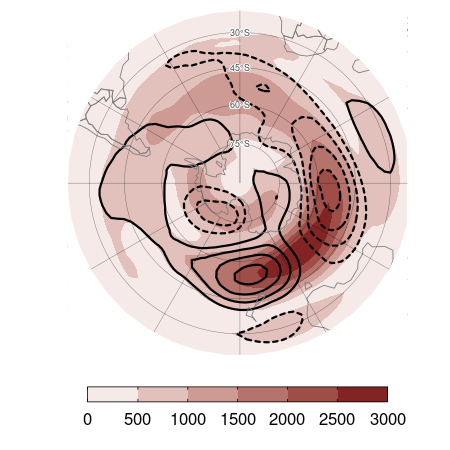
\includegraphics{figures/15-onda3/envolvente-ejemplo-1} 

}

\caption{Anomalías zonales de altura geopotencial (m) en 500 hPa en septiembre de 1989 (contornos, líneas sólidas indican valores positivos y líneas punteadas indican valores negativos) y envolvente de ondas zonales (sombreado).}\label{fig:envolvente-ejemplo}
\end{figure}



La Figura \ref{fig:envolvente-ejemplo} muestra un ejemplo de la envolvente de la ondas zonales para la altura geopotencial en 500 hPa en septiembre de 1989 junto con las anomalías zonales correspondientes.
Estas anomalías son intensas al sur de Australia y Nueva Zelanda y la envolvente captura esa región.

\hypertarget{software}{%
\subsection{Software}\label{software}}

El análisis de datos se realizó utilizando el lenguaje de programación R (\protect\hyperlink{ref-rcoreteam2020}{R Core Team, 2020}), con los paquetes data.table (\protect\hyperlink{ref-dowle2020}{Dowle and Srinivasan, 2020}) y metR (\protect\hyperlink{ref-campitelli2020}{Campitelli, 2020}).
Los gráficos se hicieron con ggplot2 (\protect\hyperlink{ref-wickham2009}{Wickham, 2009}).

Los datos de reanálisis fueron descargados con el paquete ecmwfr (\protect\hyperlink{ref-hufkens2020}{Hufkens, 2020}), los datos de CMIP y DAMIP se descargaron con el paquete rcmip6 (\protect\hyperlink{ref-rcmip6}{Campitelli, 2023}) y los índices de El Niño-Oscilación del Sur (ENSO, por sus siglas en inglés) y el dipolo del Índico, con el paquete rsoi (\protect\hyperlink{ref-albers2020}{Albers and Campitelli, 2020}).

La tesis se compiló utilizando knitr y rmarkdown (\protect\hyperlink{ref-allaire2020}{Allaire et al., 2020}; \protect\hyperlink{ref-xie2015}{Y. Xie, 2015}).

\hypertarget{resultados}{%
\section{Resultados}\label{resultados}}

\hypertarget{uxedndice-r04-1}{%
\subsection{Índice R04}\label{uxedndice-r04-1}}

La Figura \ref{fig:raphael-regr} presenta la regresión lineal entre R04 y la anomalía zonal de altura geopotencial en 500 hPa junto con la onda 3 obtenida de la descomposición de Fourier del campo medio climatológico de la altura geopotencial en 500 hPa para el período 1979--2020.
La figura incluye además las ubicaciones definidas por M. N. Raphael (\protect\hyperlink{ref-raphael2004}{2004}) para calcular el índice.
Se observa que R04 representa una onda 3 relativamente pura con una amplitud ligeramente más alta en la región del Pacífico Sur.
Sin embargo, se puede notar que los máximos al sur de Nueva Zelanda y sobre el pasaje de Drake se encuentran más al sur que los puntos usados de referencia.

\begin{figure}

{\centering 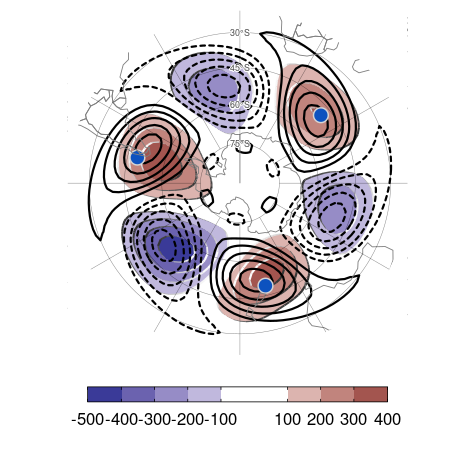
\includegraphics{figures/15-onda3/raphael-regr-1} 

}

\caption{Regresión lineal entre R04 y la anomalía zonal de altura geopotencial (m) en 500 hPa (sombreado). La onda 3 obtenida de la descomposición de Fourier del campo medio climatológico de la altura geopotencial en 500 hPa se muestra en contornos; (valores positivos en línea llena y negativos en línea punteada). En azul se indican la ubicación de los puntos usado para calcular R04.}\label{fig:raphael-regr}
\end{figure}



La onda 3 descrita por R04 coincide bien con la onda 3 climatológica, lo cual es esperable por construcción.
Al usar puntos fijos cercanos a estos máximos climatológicos, el índice R04 busca medir la similitud del campo de anomalías zonales de altura geopotencial con la onda 3 climatológica.

\begin{figure}

{\centering 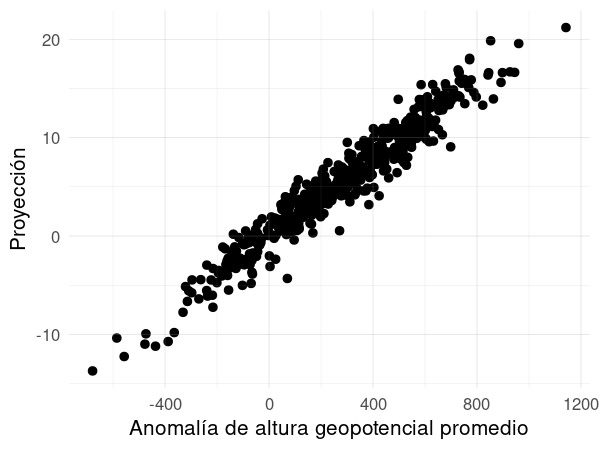
\includegraphics{figures/15-onda3/pseudo-raphael-1} 

}

\caption{Relación entre la anomalía zonal de altura geopotencial (m) en los tres puntos utilizados para construir R04 y la amplitud de la proyección de la altura geopotencial (m) en 50ºS y 500 hPa con la onda 3 climatológica}\label{fig:pseudo-raphael}
\end{figure}



La Figura \ref{fig:pseudo-raphael} muestra la relación entre la proyección de la altura geopotencial en 50ºS con la onda 3 climatológica en esa latitud y la anomalía zonal de altura geopotencial promediada en las tres ubicaciones de R04 (que no es exactamente el índice R04 ya que éste se calcula a partir de un promedio móvil de 3 meses y una estandarización previa al promediado).
Ambas series son casi idénticas, con una correlación de 0,97 (CI: 0,96 -- 0,97).
Esto ilustra que el R04 no es un índice de la amplitud de la onda 3, sino un índice de cuánto se parece la altura geopotencial en 50ºS a la onda 3 media en 50ºS.

Si bien la Figura \ref{fig:raphael-regr} muestra que R04 está asociado con una onda 3 relativamente pura, no es sorprendente que un índice basado en el promedio de 3 puntos esté altamente correlacionado con regiones cercanas a esos puntos.
Esto no garantiza que esta estructura así definida represente un patrón físicamente coherente.

\begin{table}

\caption{\label{tab:raphael-correlation}Correlación temporal entre la anomalía zonal de geopotential para cada posible par de ubicaciones (indicadas por su longitud) de los tres puntos utilizados para construir R04.}
\centering
\begin{tabular}[t]{cccc}
\toprule
 & 50°E & 165°E & 75°O\\
\midrule
50°E & 1,00 & 0,15 & -0,13\\
165°E & 0,15 & 1,00 & 0,04\\
75°O & -0,13 & 0,04 & 1,00\\
\bottomrule
\end{tabular}
\end{table}

Para explorar la consistencia física de la aplicación de R04 se presenta la Tabla \ref{tab:raphael-correlation}, que muestra la matriz de correlación entre la anomalía zonal de altura geopotencial en las ubicaciones utilizadas para calcular R04, indicadas por su longitud.
Las correlaciones son muy cercanas a cero, e incluso la correlación entre el punto de 75ºO y 50ºE es negativa.
Esto indica que los puntos no son covariantes, lo que implica que no serían parte de un mismo patrón de onda coherente.

\begin{figure}

{\centering 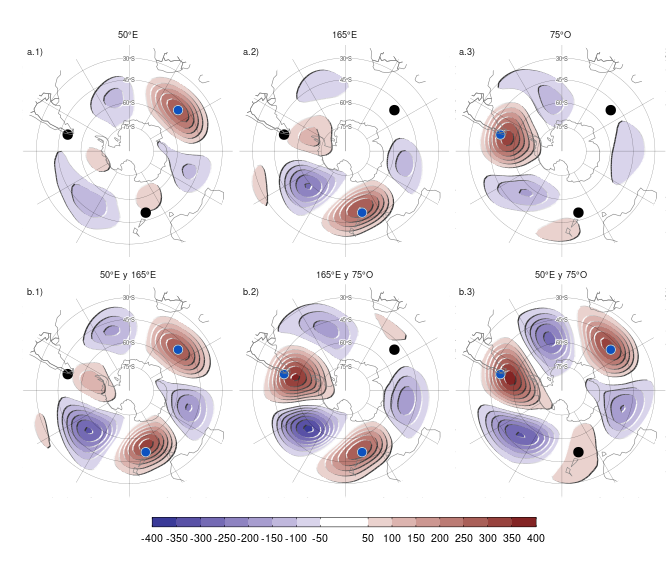
\includegraphics{figures/15-onda3/cor-puntos-1} 

}

\caption{Regresión entre las anomalías zonales de altura geopotencial en 500 hPa e índices R04 usando combinaciones de 1 y 2 puntos (m). En cada panel, los puntos azules son los puntos usados para calcular el índice y los negros, los excluidos.}\label{fig:cor-puntos}
\end{figure}



La Figura \ref{fig:cor-puntos} muestra los campos de regresión entre la anomalía zonal de altura geopotencial e índices similares a R04 pero computados considerado o bien solo un punto (Fig. \ref{fig:cor-puntos}, fila a) o promedios de combinaciones de dos puntos (Fig.\ref{fig:cor-puntos}, fila b) de los tres utilizados para computar R04.
La figura muestra que no se encuentra un patrón coherente de onda 3 asociado a los puntos individuales.
Por otra parte, los campos obtenidos a partir de las combinaciones de dos puntos se asocian a anomalías positivas en los dos puntos relevantes y negativas entre los mismos --esperable ya que se trata de anomalías zonales-- pero, crucialmente, no hay una asociación positiva con el tercer punto no incluido en el índice.

\begin{figure}

{\centering \subfloat[Meses con mayor valor de R04\label{fig:raphael-top8-1}]{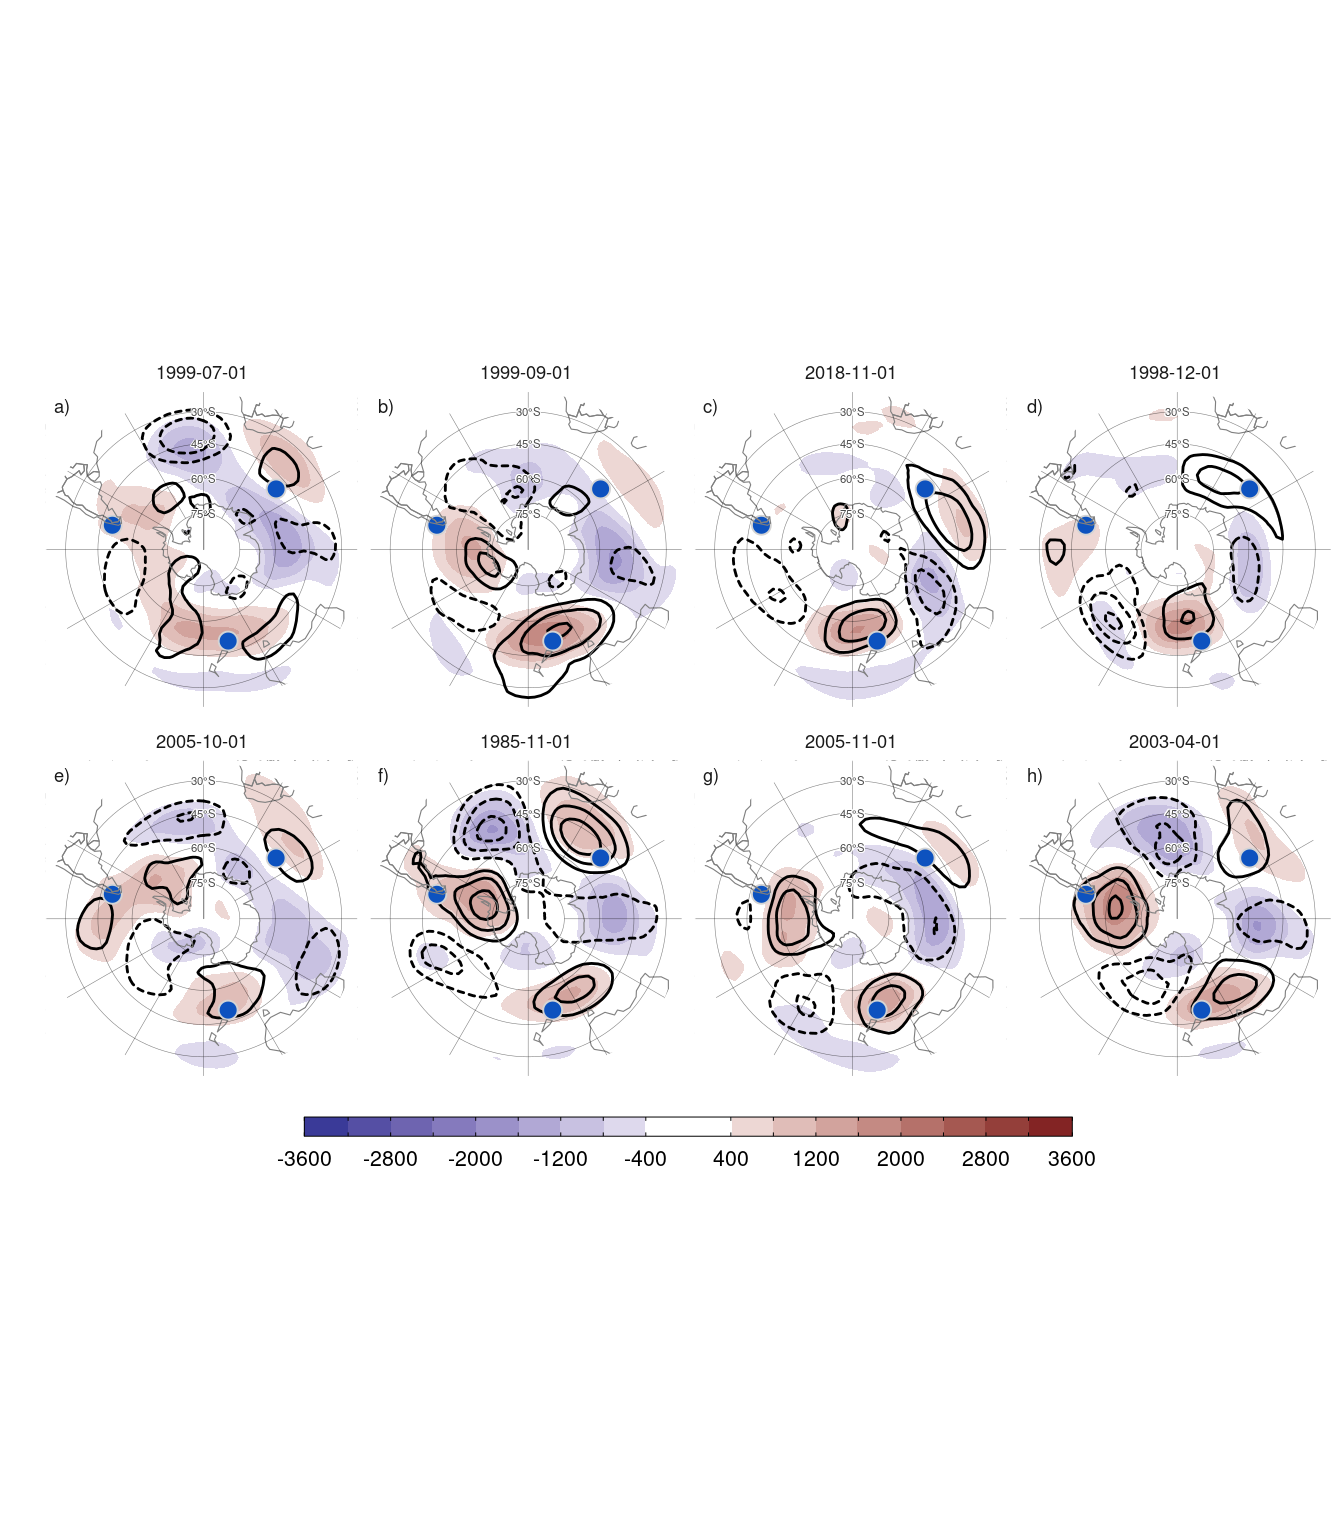
\includegraphics{figures/15-onda3/raphael-top8-1} }\newline\subfloat[Meses con menor valor de R04\label{fig:raphael-top8-2}]{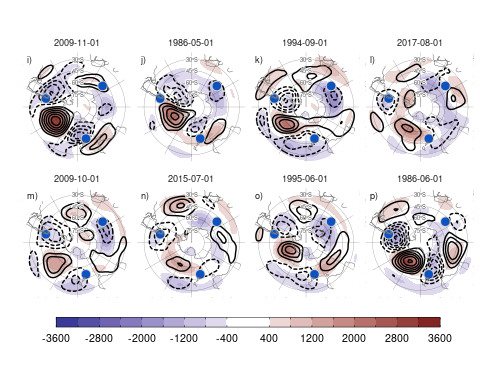
\includegraphics{figures/15-onda3/raphael-top8-2} }

}

\caption{Anomalía zonal de altura geopotencial (m, sombreado) y anomalía mensual de la anomalía zonal de altura geopotencial (m, contornos, valores positivos en línea sólida y valores negativos en línea punteada) en 500 hPa para los 8 meses con mayor y menor valor del índice R04. Los puntos azules indican las ubicaciones usadas en el índice R04.}\label{fig:raphael-top8}
\end{figure}



Finalmente, las Figuras \ref{fig:raphael-top8-1} y \ref{fig:raphael-top8-2} muestran las anomalías mensuales zonales de la altura geopotencial para los 8 meses con mayor y menor valor del índice R04, respectivamente.
En pocos casos se observa un patrón de onda 3 bien marcado; por ejemplo, en abril de 2003 y noviembre de 1985 (paneles f y g) se observan tres zonas de anomalías positivas cercanas a las ubicaciones utilizadas para calcular R04 y tres zonas de anomalías negativas entre las mismas.
En octubre de 2009 (panel m) se observa lo contrario.
En casos para los cuales el índice es grande y positivo no hay siquiera anomalías positivas en los tres puntos, como en noviembre de 2018 (panel b) y diciembre de 1998 (panel e).
En los meses con menores valores del índice R04, parece haber un patrón de onda tipo PSA algo más definido, sin embargo, tampoco en estos casos hay buena consistencia entre los puntos.

De este análisis se desprende que el índice propuesto por M. N. Raphael (\protect\hyperlink{ref-raphael2004}{2004}) no sería capaz de representar las características espacio-temporales de la onda 3.

\hypertarget{descomposiciuxf3n-de-fourier}{%
\subsection{Descomposición de Fourier}\label{descomposiciuxf3n-de-fourier}}

Otra forma de cuantificar la actividad de la onda 3 es, como se mencionó previamente, computando la amplitud obtenida a través de una descomposición de Fourier para este número de onda a lo largo de un círculo de latitud.
Este método también asume que la onda 3 tiene una amplitud constante a lo largo de todo el círculo de latitud y que no presenta dispersión meridional.
Esta metodología no mide exactamente lo mismo que R04, ya que en este caso es sensible a la amplitud de la onda 3 sin importar dónde esté localizada.
Esto puede observarse en la Figura \ref{fig:fase-histogram}, que presenta un histograma de la fase de la onda 3 obtenida a partir de la descomposición de Fourier de la altura geopotencial y que muestra que la localización de la onda varía considerablemente.
También se puede observar el ciclo anual de la fase.

\begin{figure}

{\centering 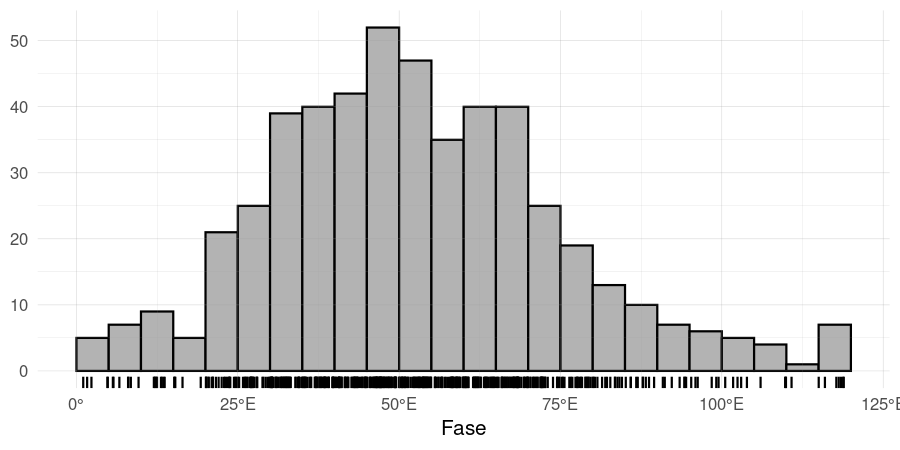
\includegraphics{figures/15-onda3/fase-histogram-1} 

}

\caption{Histograma de la fase de la onda 3 de altura geopotencial en 500 hPa para cada trimestre.}\label{fig:fase-histogram}
\end{figure}



Por otro lado, cabe mencionar que la onda 3 que se obtiene de la descomposición de Fourier aplicada directamente a las medias mensuales de la altura geopotencial no es idéntica a la onda 3 que surge de la descomposición de Fourier aplicada a las anomalías mensuales de altura geopotencial mensual.
Dado que la variable relevante para estudiar la variabilidad, los impactos, los forzantes y las tendencias son las anomalías con respecto a la media, desde ahora se analizarán las anomalías mensuales.

\begin{figure}

{\centering 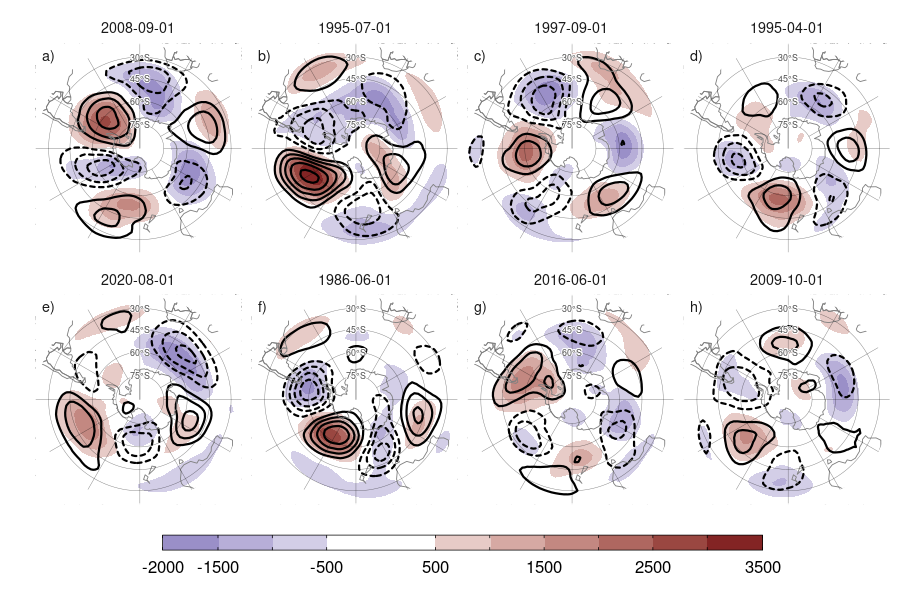
\includegraphics{figures/15-onda3/zw3-top8-1} 

}

\caption{Anomalía zonal de altura geopotencial (m, sombreado) y anomalía mensual de la anomalía zonal de altura geopotencial (m, contornos, valores positivos en línea sólida y valores negativos en línea punteada) en 500 hPa para los 8 meses con mayor y menor valor de la amplitud de la onda 3 de la anomalía mensual de altura geopotencial en 500 hPa}\label{fig:zw3-top8}
\end{figure}



La Figura \ref{fig:zw3-top8} presenta las anomalías zonales y mensuales de altura geopotencial en 500 hPa, para los 8 meses con mayor amplitud de la onda 3 de las anomalías mensuales de altura geopotencial en 50ºS.
Algunos meses, como septiembre de 1997, abril de 1995 y octubre de 2009 (Fig. \ref{fig:zw3-top8}, paneles c, d y h) tienen máximos y mínimos de intensidad relativamente constante.
En la mayoría, aún cuando se puede observar una onda 3 relativamente clara, su amplitud no es constante a lo largo de todo el hemisferio.
Por ejemplo, en septiembre de 2008 (Fig. \ref{fig:zw3-top8}, panel a), las anomalías zonales tienen mayor intensidad y se encuentran más al sur en la zona del Pacífico y al este de Sudamérica que en el Índico y al sur de Australia.
En cambio, en junio de 1986 (Fig. \ref{fig:zw3-top8}, panel f) las anomalías tienen mayor intensidad en la zona del Pacífico y al sur de Australia y son casi nulas en el Atlántico.

\begin{figure}

{\centering 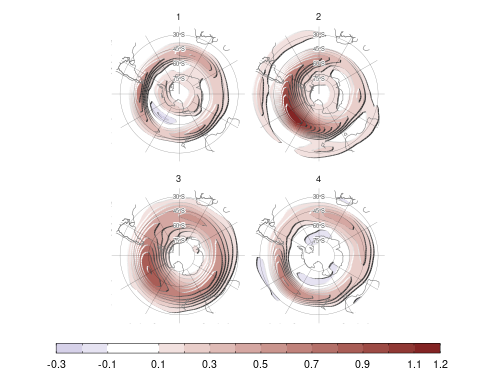
\includegraphics{figures/15-onda3/envelope-regr-1} 

}

\caption{Regresión entre la amplitud de las ondas 1 a 4 y la envolvente de todas las ondas zonales de las anomalías de altura geopotencial (sin unidades).}\label{fig:envelope-regr}
\end{figure}



Esta diferencia longitudinal en la amplitud de las ondas puede capturarse a partir de la envolvente de las ondas.
La Figura \ref{fig:envelope-regr} muestra la regresión entre la amplitud de las ondas 1 a 4 y la envolvente de todas las ondas zonales de las anomalías de altura geopotencial.
Se observa que la amplitud de la onda 1 se asocia a mayor actividad de onda en una banda aproximadamente zonalmente simétrica, indicando que la onda 1 contribuye con las anomalías zonales aproximadamente en todas las longitudes.
Las ondas 2 y 3, en cambio, contribuyen a las anomalías mensuales de altura geopotencial principalmente en el Pacífico sur.
Esto es consistente con lo observado en los casos particulares en la Figura \ref{fig:zw3-top8} y sugiere que la onda 3 puede presentar variaciones longitudinales que no son capturadas por un modelo sinusoidal puro.

\hypertarget{conclusiones-del-capuxedtulo-refonda3}{%
\section{Conclusiones del capítulo \ref{onda3}}\label{conclusiones-del-capuxedtulo-refonda3}}

De este análisis se concluye que ni el modelo de M. N. Raphael (\protect\hyperlink{ref-raphael2004}{2004}) ni el modelo de Fourier son adecuados para describir las variaciones espacio-temporales de la onda 3 en el hemisferio sur.
Es necesario entonces una metodología que permita describir cambios en la fase, modulación zonal de la amplitud y propagación meridional.
En el próximo capítulo se presenta un índice basado en cEOF que apunta a resolver estos problemas.

\hypertarget{ceofs}{%
\chapter{Modos de variabilidad de la circulación zonalmente asimétrica en primavera}\label{ceofs}}

\hypertarget{introducciuxf3n}{%
\section{Introducción}\label{introducciuxf3n}}

Dadas las deficiencias de los índices analizados previamente, es necesaria una metodología alternativa para caracterizar la circulación zonalmente asimétrica.
Se propone el uso de cEOFs (\protect\hyperlink{ref-horel1984}{Horel, 1984}), ya que éstas permiten caracterizar modos de variabilidad con amplitud y fase variable en el tiempo y con una estructura espacial más compleja que la que presentan ondas sinusoidales constantes por cada círculo de latitud.

En este capítulo el estudio se restringe al trimestre septiembre-octubre-noviembre (SON) ya que durante esta estación las teleconexiones sobre Sudamérica son más intensas (\protect\hyperlink{ref-cazes-boezio2003}{Cazes-Boezio et al., 2003}) y es de interés de esta tesis estudiar las características de la circulación del hemisferio sur de influencia en esa región.
Muchas de las características de los patrones que se obtienen a través de cEOF son similares en los otros trimestres a excepción del trimestre diciembre-enero-febrero, en el cual las ondas zonales están menos organizadas.

Se analizó el nivel de 200 hPa dado que, como se mencionó en la Introducción, es alrededor de este nivel donde se encuentra el máximo de la amplitud de la onda 3 (\protect\hyperlink{ref-campitelli2018b}{Campitelli, 2018}).
Asimismo, dada la importancia de la variabilidad estratosférica en modular la propagación de las ondas, también se incluye el nivel de 50 hPa.

\hypertarget{muxe9todos-1}{%
\section{Métodos}\label{muxe9todos-1}}

\hypertarget{datos-1}{%
\subsection{Datos}\label{datos-1}}

Se utilizan datos mensuales de ERA5 al igual que en el capítulo anterior.
Además de la altura geopotencial, se utilizan datos de temperatura del aire y relación de mezcla de ozono y los 37 niveles estándard del reanálisis, temperatura del aire a 2 metros y columna total de ozono (CTO).
La mayor parte del análisis utiliza datos del período post-satelital (1979--2020), aunque también en algunos resultados se extienden hasta 1940 para examinar las tendencias a largo plazo.

El análisis también utiliza la función corriente en 200 hPa que se derivó a partir de la vorticidad de ERA5 utilizando la subrutina de FORTRAN FISHPACK (\protect\hyperlink{ref-fishpack}{Adams et al., 1999}), y con los flujos horizontales de actividad de onda que se calcularon siguiendo el método descrito por Plumb (\protect\hyperlink{ref-plumb1985}{1985}).

Para analizar la influencia del océano superficial en la circulación, se utiliza datos mensuales de Temperatura de la Superficie del Mar (TSM) del conjunto Extended Reconstructed Sea Surface Temperature (ERSST) v5 (\protect\hyperlink{ref-huang2017}{Huang et al., 2017}) con una resolución de 2º.

También se utiliza la precipitación mensual del CPC Merged Analysis of Precipitation (CMAP, \protect\hyperlink{ref-xie1997}{P. Xie and Arkin, 1997}), con una resolución de 2,5º.
Este conjunto de datos de lluvia integra información de diversas fuentes, incluyendo observaciones de pluviómetros, estimaciones inferidas por satélite y el reanálisis NCEP-NCAR.

Además, se incorporaron índices climáticos en nuestro análisis.
El Índice del ENSO Oceánico (ONI, \protect\hyperlink{ref-bamston1997}{Bamston et al., 1997}) utilizando en forma operativa por el Climate Prediction Center de la NOAA y el Índice del Dipolo del Índico (DMI, \protect\hyperlink{ref-saji2003}{Saji and Yamagata, 2003}) del Global Climate Observing System Working Group on Surface Pressure.

\hypertarget{regresiones}{%
\subsection{Regresiones}\label{regresiones}}

Para cuantificar la asociación entre múltiples índices o índices multivariados y otras variables meteorológicas se utilizó regresión lineal múltiple.
Para obtener los coeficientes lineales de una variable \(Z\) (altura geopotencial, temperatura, precipitación, etc.) con un índice de variables X e Y se ajustó la ecuación

\begin{equation}
Z(\lambda, \phi, t) = \alpha(\lambda, \phi) \operatorname{X} + \beta(\lambda, \phi) \operatorname{Y} + X_0(\lambda, \phi) + \epsilon(\lambda, \phi, t)
\label{eq:multiple-regression-sam}
\end{equation}

donde \(\lambda\) y \(\phi\) son la longitud y la latitud, \(t\) es el tiempo, \(\alpha\) y \(\beta\) son los coeficientes de regresión lineal, \(X_0\) y \(\epsilon\) son la constante y los términos de error.
A partir de esta ecuación, \(\alpha\) representa la asociación (lineal) de \(Z\) con la variabilidad de \(X\) que no se explica por la variabilidad de \(Y\); es decir, es proporcional a la correlación parcial de \(Z\) y \(X\), controlando el efecto de \(Y\), y viceversa para \(\beta\).

Para las regresiones estacionales, se promediaron la variables para cada año y trimestre (DEF, MAM, JJA, SON) antes de calcular la regresión.

La significancia estadística de los campos de regresión se evaluó ajustando los p-valores mediante el control de la Tasa de Falso Descubrimiento (FDR, \protect\hyperlink{ref-benjamini1995}{Benjamini and Hochberg, 1995}; \protect\hyperlink{ref-wilks2016}{Wilks, 2016}) para evitar resultados engañosos derivados del elevado número de regresiones (\protect\hyperlink{ref-katz1991}{Katz and Brown, 1991}; \protect\hyperlink{ref-walker1914}{Walker, 1914}).

Se calcularon las tendencias lineales mediante mínimos cuadrados ordinarios y el intervalo de confianza del 95\% se calculó asumiendo una distribución t con los grados de libertad de los residuos apropiados.

Se calcularon las estimaciones de probabilidad de densidad utilizando un kernel gaussiano de anchura óptima según Sheather and Jones (\protect\hyperlink{ref-sheather1991}{1991}).

\hypertarget{eof}{%
\subsection{EOF}\label{eof}}

Se calcularon los EOFs haciendo la descomposición en valores singulares de la matriz de datos.
Se ponderaron los valores por la raíz cuadrada del coseno de la latitud para tener en cuenta el área representada por cada punto de grilla (\protect\hyperlink{ref-chung1999}{Chung and Nigam, 1999}).

La Figura \ref{fig:eof-naive} muestra las cuatro primeras EOFs de las anomalías zonales de altura geopotencial de SON en 50 hPa al sur de 20º S.
Se puede observar que los dos primeros EOFs representan un patrón de onda zonal 1 con los centros ubicados en fase de cuadratura, es decir, girados en 1/4 de longitud de onda (90º en el espacio de frecuencias).
Esto implica que la onda 1 es un patrón no estacionario (es decir, un patrón con características espaciales similares donde la localización de los máximos varía).
Esto se debe a que los EOFs estándar sólo pueden representar patrones estacionarios (\protect\hyperlink{ref-horel1984}{Horel, 1984}), mientras que pueden representar patrones no estacionario solamente a partir de la combinación de pares de EOFs.
La amplitud de esta onda 1 podría medirse entonces como \(\sqrt{\mathrm{PC1}^2 + \mathrm{PC2}^2}\) y su fase como \(\tan^{-1} \left ( \frac{\mathrm{PC2}}{\mathrm{PC1}} \right )\) (donde PC1 y PC2 son las series temporales asociadas a cada EOF).
Lo mismo sucede con el siguiente par de EOFs (EOF3 y EOF4), los cuales representan un mismo patrón con una escala espacial menor.
Esto se fundamenta en la inspección visual cualitativa de estos patrones espaciales y sólo funciona correctamente si ambas fases aparecen claramente divididas en estos dos EOFs, lo cual no está garantizado por construcción.

Las series temporales del Patrón del Pacífico-Sudamérica 1 y 2 (PSA1 y PSA2) fueron computadas como el segundo y tercer EOF de la anomalía de altura geopotencial trimestral en 500 hPa usando todos los trimestres siguiendo a Mo and Paegle (\protect\hyperlink{ref-mo2001}{2001}).

\hypertarget{ceof-metodo}{%
\subsection{Funciones ortogonales complejas (cEOF)}\label{ceof-metodo}}

Una alternativa para representar ondas que varían en su fase es utilizando el análisis de cEOF (\protect\hyperlink{ref-horel1984}{Horel, 1984}).
Cada cEOF es un conjunto de estructuras espaciales y series temporales con valores en el plano complejo (es decir, con una parte real y una imaginaria) de la forma

\begin{align}
E_{(\lambda, \phi, p)} &= (E_{r(\lambda, \phi, p)} +  iE_{i(\lambda, \phi, p)}) \\
T_{(t)} &= (T_{r(t)} +  iT_{i(t)})
\label{eq:ceof-equation}
\end{align}

donde \(E_{(\lambda, \phi)}\) es la componente espacial del cEOF, que depende de la longitud (\(\lambda\)), la latitud (\(\phi\)) y el nivel de presión (\(p\)) y que tiene una parte real \(E_r\) y una imaginaria \(E_i\).
\(T_{(t)}\) es la parte temporal del cEOF, al cual también tiene una parte real \texttt{T\_\{r(t)\}} y una imaginaria \texttt{T\_\{i(t)\}}
La contribución de cada cEOF al campo original se obtiene como la parte real del producto entre las componentes espacial y temporal.



\begin{figure}

{\centering 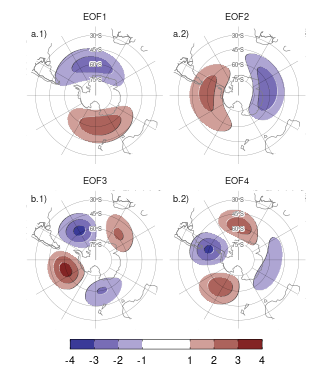
\includegraphics{figures/20-ceofs/eof-naive-1} 

}

\caption{Patrones espaciales de los primeros EOFs de las anomalías zonales de altura geopotencial en 50 hPa al sur de 20ºS. Para el período 1979--2020. Unidades arbitrarias.}\label{fig:eof-naive}
\end{figure}

Las componentes real e imaginaria del patrón espacial complejo son la representación de dos patrones espaciales que están desplazados 1/4 de longitud de onda, similar a EOF1 y EOF2 en la Figura \ref{fig:eof-naive}.
En este trabajo la parte real e imaginaria de cada cEOF se referirán como la fase de 0º y la fase de 90º respectivamente.
El campo real reconstruido por cada cEOF es la combinación lineal de los dos campos espaciales ponderados por sus respectivas series temporales.
Esto es análogo a cómo cualquier onda sinusoidal de fase y amplitud arbitraria puede construirse mediante la suma de un seno y un coseno de diferente amplitud pero fase fija.
Esto permite que los cEOF representen patrones ondulatorios que cambian tanto su fase como su amplitud.

\begin{figure}

{\centering 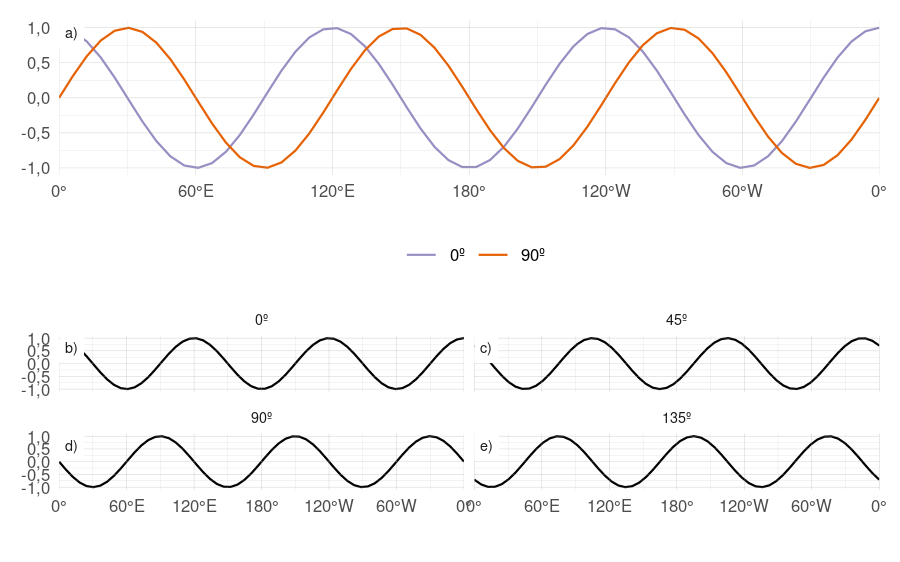
\includegraphics{figures/20-ceofs/ejemplo-reconstruccion-1} 

}

\caption{Ejemplo idealizado de las dos fases del patrón espacial de un cEOF (fila superior) y cuatro reconstrucciones para distintos valores de sus series temporales.}\label{fig:ejemplo-reconstruccion}
\end{figure}



Un ejemplo idealizado se presenta en la Figura \ref{fig:ejemplo-reconstruccion}, la cual representa la parte espacial de las fases de 0º y 90º de un cEOF hipotético en el panel superior y cuatro reconstrucciones de la variable original en el panel inferior.
Cuando la serie temporal de la fase de 0º es positiva y la serie temporal de la fase 90º es cercana a cero, entonces las anomalías zonales de altura geopotencial son similares al patrón espacial de la fase de 0º (panel b).
Del mismo modo, cuando la serie temporal de la fase 0º es cercana a cero y la serie la serie temporal de la fase de 90º es positiva, entonces las anomalías zonales de altura geopotencial se parecen a la fase de 90 (panel d).
Cuando ambas fases de la serie temporal son distintas a cero, entonces las anomalías zonales de altura geopotencial tiene los máximos en una localización intermedia (paneles c y e).

El signo de los EOF tradicionales no está determinado unívocamente, por lo que se puede multiplicar cada EOF por -1 (tanto su serie temporal como su patrón espacial) y obtener una descripción igualmente válida.
Este cambio de signo en los números reales corresponde a una rotación en el plano complejo de 0 o \(\pi\).
De forma similar, los cEOF no tienen un argumento (entendiendo los números complejos como una magnitud y un argumento) definido, por lo que pueden rotarse en el plano complejo con cualquier ángulo entre 0 y \(2\pi\) (\protect\hyperlink{ref-horel1984}{Horel, 1984}); esto es una multiplicación por \(\cos(\alpha) + i\sin(\alpha)\) con \(\alpha\) cualquier número real entre 0 y \(2\pi\).

El procedimiento para calcular los cEOF es similar al de computar los EOF con la única diferencia de que los datos de entrada primero se convierten en su señal analítica.
Ésta señal es un número complejo cuya parte real es la serie original y cuya parte imaginaria son los datos originales desplazados 90º en cada frecuencia espectral, es decir, su transformada de Hilbert.
La transformada de Hilbert suele entenderse en términos de una señal variable en el tiempo, pero las ondas zonales son estructuras con forma de onda en el sentido zonal.
Por esto se calculó la transformada de Hilbert de las anomalías zonales de altura geopotencial variable en cada longitud; es decir, calculada para cada nivel, tiempo y latitud.
Dado que cada círculo de latitud es un dominio periódico, este procedimiento no sufre efectos de borde.



\begin{figure}

{\centering 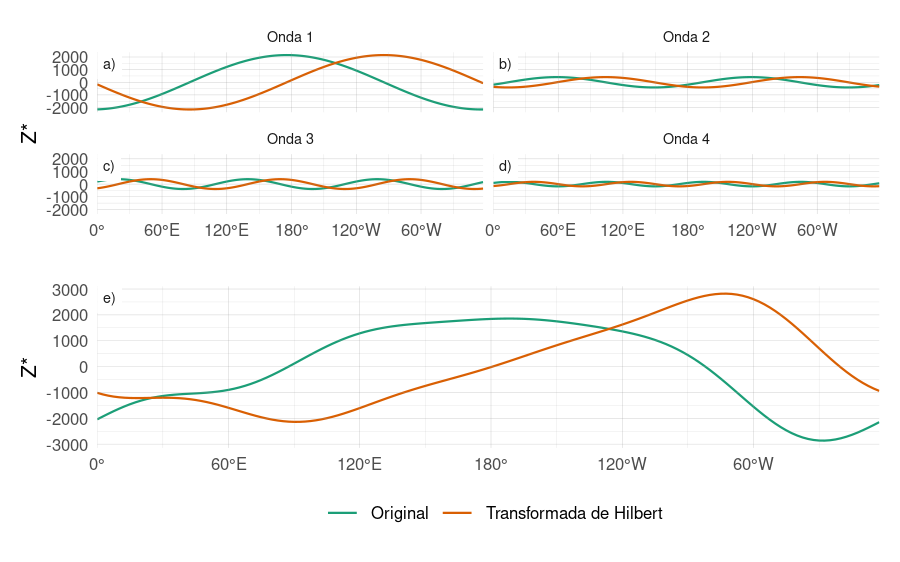
\includegraphics{figures/20-ceofs/hilbert-ejemplo-1} 

}

\caption{Ejemplo de cálculo de la función analítica de la señal de anomalías zonales de altura geopotencial (m) en 50ºS en SON de 1982. Las anomalías zonales (línea verde en panel e) se pueden descomponer en un número de ondas zonales (paneles a, b, c y d muestran las primeras 4 en verde). La transformada de Hilbert de las anomalías zonales de altura geopotencial (línea naranja en panel e) es la suma de las ondas zonales desplazadas en 1/4 de longitud de onda (líneas naranjas en paneles a, b, c, y d).}\label{fig:hilbert-ejemplo}
\end{figure}

La Figura \ref{fig:hilbert-ejemplo} ilustra la señal analítica con las anomalías zonales de geopotencial de SON en 1982 en 50hPa y 50ºS donde la línea verde es la señal original y la línea naranja es la transformada de Hilbert.
En los paneles superiores la señal está dividida en las ondas zonales 1 a 4 donde se ve con claridad como la transformada de Hilbert es la misma señal pero desplazada 1/4 de longitud de onda.



\begin{table}

\caption{\label{tab:corr-ceof-splitted}Coeficiente de determinación (\(r^2\)) entre la magnitud de las series temporales de los primeros tres cEOFs computados de forma separada en 50 y 200 hPa (p-valores menores a 0,01 en negrita).}
\centering
\begin{tabular}[t]{l>{}r>{}r>{}r}
\toprule
\multicolumn{1}{c}{} & \multicolumn{3}{c}{50 hPa} \\
\cmidrule(l{3pt}r{3pt}){2-4}
200 hPa & cEOF1 & cEOF2 & cEOF3\\
\midrule
cEOF1 & \textbf{0,29} & 0,01 & 0,03\\
cEOF2 & 0,00 & \textbf{0,59} & 0,02\\
cEOF3 & 0,00 & 0,00 & 0,01\\
\bottomrule
\end{tabular}
\end{table}

Se calcularon los cEOFs de las anomalías zonales de geopotencial en los niveles de 50 y 200 hPa al sur de 20ºS por separado en el período 1979--2020.
La Tabla \ref{tab:corr-ceof-splitted} muestra el coeficiente de determinación de la magnitud de las series temporales de los cEOF entre 50 y 200 hPa.
Una correlación significativa entre la magnitud de los respectivos cEOF1 y cEOF2 en cada nivel.
Los patrones espaciales de los cEOF de 50 hPa y 200 hPa también son similares (no se muestra).

Tanto la similitud del patrón espacial como la alta correlación temporal de los cEOF calculados a 50 hPa y 200 hPa sugieren que se trata, en gran medida, de modos de variabilidad conjunta.
Esto motivó calcular los cEOF en ambos niveles conjuntamente.
El resultado es que cada cEOF tiene una componente espacial que depende de la longitud, la latitud y el nivel, y una componente temporal que sólo depende del tiempo.
Dada las diferencias de magnitud entre la variabilidad de la altura geopotencial en 50 hPa y 200 hPa, se estandarizaron las variables de cada nivel por su desvío estándar.

Como se mencionó anteriormente, el argumento de los cEOF no está determinado unívocamente y se le puede sumar una constante real arbitraria.
Para facilitar la interpretación y permitir la reproducibilidad, se define el argumento de cada cEOF de modo que alguna de las dos fases esté alineada con alguna variable significativa de nuestro análisis.
Este procedimiento no crea correlaciones espurias, sólo toma una relación existente y la alinea con una fase específica.

Un análisis preliminar mostró que el cEOF1 está estrechamente relacionado con la onda zonal 1 de la Columna Total de Ozono (CTO) y el cEOF2 está estrechamente relacionado con el ENSO.
Por lo tanto, se eligió el argumento del cEOF1 de forma que la serie temporal correspondiente al cEOF1 de 0º tenga la máxima correlación con la onda zonal 1 del CTO entre 75°S y 45°S.
Del mismo modo, se eligió el argumento del cEOF2 de modo que el coeficiente de determinación entre el ONI y el cEOF2 de 0º sea mínimo, lo que también casi maximiza la correlación con el cEOF2 de 90º.

Si bien los cEOFs se calcularon para el período 1979--2020, se extendieron las series temporales complejas hasta el periodo 1950--1978 proyectando las anomalías zonales mensuales de altura geopotencial normalizadas por nivel al sur de 20ºS sobre los patrones espaciales correspondientes.

\hypertarget{resultados-1}{%
\section{Resultados}\label{resultados-1}}

\hypertarget{caracterizaciuxf3n-espacio-temporal-de-los-ceofs-principales}{%
\subsection{Caracterización espacio-temporal de los cEOFs principales}\label{caracterizaciuxf3n-espacio-temporal-de-los-ceofs-principales}}

Las Figuras \ref{fig:ceofs-1} y \ref{fig:extended-series} muestran las partes espacial y temporal de los dos primeros cEOFs de las anomalías zonales de la altura geopotencial en 50 hPa y 200 hPa, calculados conjuntamente en ambos niveles.
El primer modo (cEOF1) explica el 82,2\% de la varianza de las anomalías zonales, mientras que el segundo modo (cEOF2) explica una fracción menor (6,9\%).
En los patrones espaciales (Fig. \ref{fig:ceofs-1}), las fases de 0º y 90º están en cuadratura por construcción, de modo que cada cEOF describe un único patrón ondulatorio cuya amplitud y fase está controlada por la magnitud y fase de su serie temporal.



\begin{figure}

{\centering 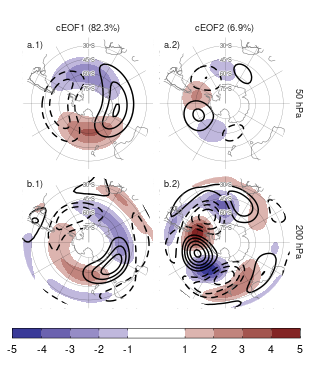
\includegraphics{figures/20-ceofs/ceofs-1-1} 

}

\caption{Patrones espaciales de los dos primeros cEOF de las anomalías zonales de altura geopotencial de SON en 50 (columna a) y 200 (columna b) hPa para el período 1979--2020. El sombreado corresponde a la fase 0º y los contornos, a la fase 90º. La proporción de varianza explicada por cada modo con respecto a la media zonal está indicada entre paréntesis. Unidades arbitrarias.}\label{fig:ceofs-1}
\end{figure}



\begin{figure}

{\centering 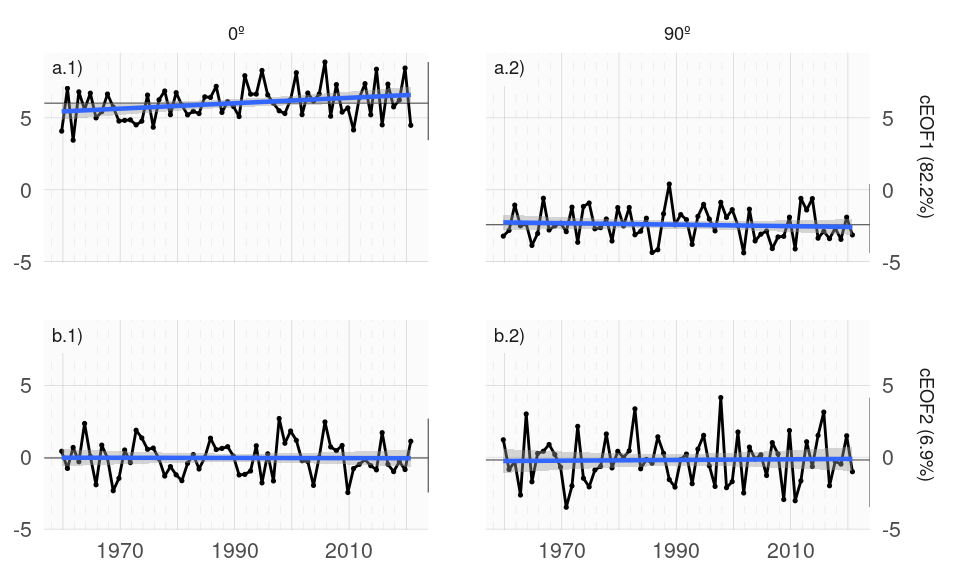
\includegraphics{figures/20-ceofs/extended-series-1} 

}

\caption{Series temporales de los dos primeros cEOF de las anomalías zonales de altura geopotencial de SON en 50 y 200 hPa para el período 1940--2020. El cEOF1 (fila a) y cEOF2 (fila b) separados en la fase 0º (columna 1) y la fase 90º (columna 2). Las líneas oscuras muestran la tendencia lineal mediante un suavizado de regresión local. Las líneas negras horizontales y verticales muestran el valor medio y el rango de cada serie, respectivamente. La proporción de varianza explicada por cada modo con respecto a la media zonal está indicada entre paréntesis. Unidades arbitrarias.}\label{fig:extended-series}
\end{figure}

El cEOF1 (Fig. \ref{fig:ceofs-1} columna 1) presenta un patrón de onda 1 con amplitud máxima en latitudes altas y en altura.
En 50 hPa la fase de 0º del cEOF1 tiene el máximo de la onda 1 en 150ºE y en 200 hPa el máximo se sitúa en torno a 175ºE indicando un desplazamiento hacia el oeste con la altura.
El cEOF2 (Fig. \ref{fig:ceofs-1} columna 2) muestra también una estructura de onda zonal con amplitud máxima en latitudes altas, pero con escalas espaciales más cortas.
En particular, la estructura dominante a ambos niveles es una onda 3 pero con mayor amplitud en el sector del océano Pacífico.
No hay cambio de fase o desplazamiento aparente con la altura, pero la amplitud del patrón se reduce considerablemente en la estratosfera, lo que es coherente con el hecho de que el cEOF2 calculado por separado para 200 hPa explica un porcentaje mayor de la varianza que el cEOF2 calculado por separado para 50 hPa (11\% vs.~3\%, respectivamente).
Esto sugiere que este modo barotrópico está asociado principalmente con la variabilidad troposférica.

No se encontró una correlación significativa entre las series temporales del cEOF1 y el cEOF2 en ninguna fase (no se muestra).
Ambos cEOF muestran variabilidad interanual pero no muestran evidencia de variabilidad decadal (Fig. \ref{fig:extended-series}).
Debido a que los campos que entran en el algoritmo de cEOF son anomalías con respecto a la media zonal en lugar de la media temporal, las series temporales de los cEOF tienen media temporal no nula.
Sin embargo, la media temporal de cEOF2 es casi cero, lo que indica que sólo el cEOF1 incluye variabilidad que se proyecta significativamente sobre el campo anómalo zonal medio.
Esto es coherente con el hecho de que el campo medio zonalmente anómalo de la altura geopotencial es muy similar al cEOF1 (\(r^2\) = 98\%) y no es similar al cEOF2 (\(r^2\) = 0\%).

La fase de 0º del cEOF1 evidencia una variación a largo plazo, con valores generalmente negativos al comienzo del período y positivos al final (Fig. \ref{fig:extended-series}a.1, p-valor de la tendencia lineal = 0,0024).
Esta tendencia positiva parece haber desparecido luego de 2000 a indica un aumento de la magnitud de la onda zonal 1 de latitudes altas.
Por otra parte, no se encuentran tendencias significativas en ninguna de las fases de cEOF2.

\hypertarget{mapas-de-regresiuxf3n-a-partir-de-los-ceof}{%
\subsection{Mapas de regresión a partir de los cEOF}\label{mapas-de-regresiuxf3n-a-partir-de-los-ceof}}

\hypertarget{altura-geopotencial}{%
\subsubsection{Altura geopotencial}\label{altura-geopotencial}}

En la sección anterior se mostraron los patrones espaciales de los cEOF obtenidos a partir de las anomalías zonales de altura geopotencial.
En esta sección se calculan campos de regresión entre las series temporales de los cEOF y las anomalías temporales de altura geopotencial para describir la influencia de los cEOF en las anomalías temporales.



\begin{figure}

{\centering 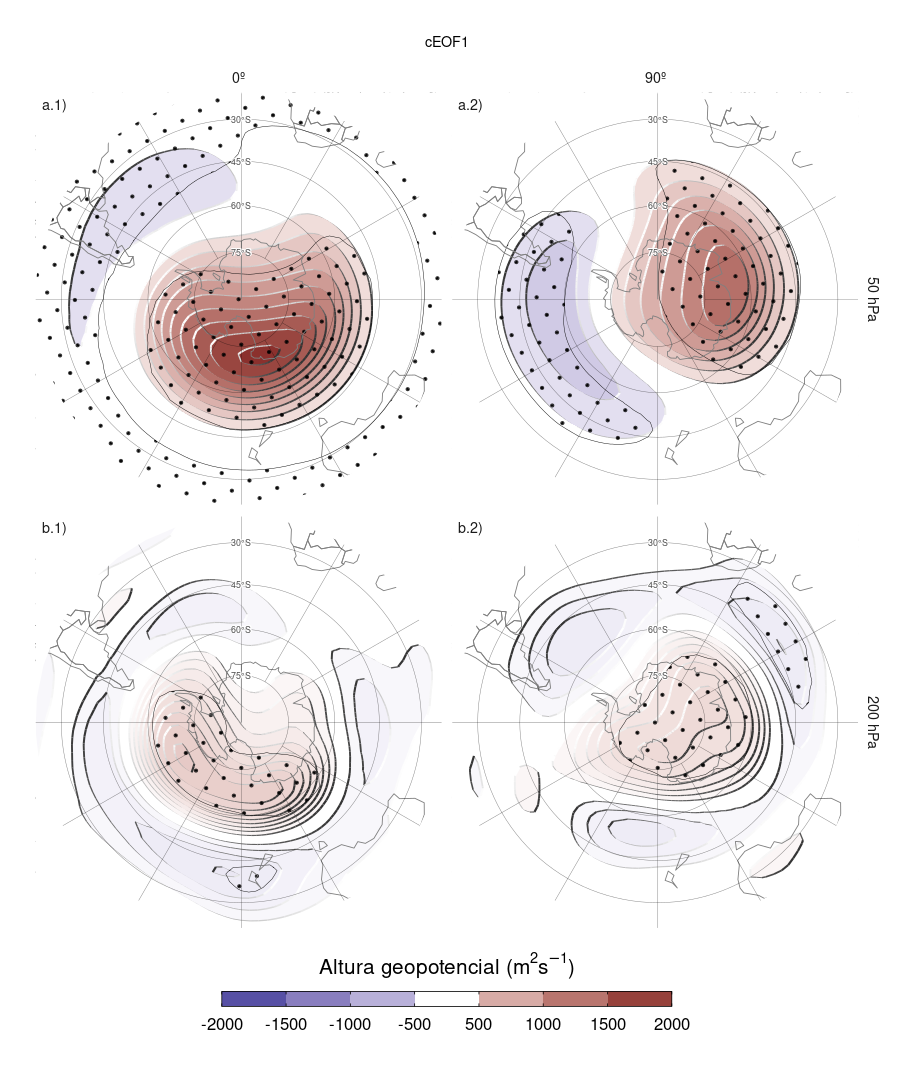
\includegraphics{figures/20-ceofs/eof1-regr-gh-1} 

}

\caption{Regresión de anomalías de altura geopotencial en SON (m) con la fase de 0º (columna 1) y de 90º (columna 2) del cEOF1 en 50 hPa (fila a) y 200 hPa (fila b) para el período 1979--2020. Estos coeficientes fueron obtenidos a partir de una regresión múltiple incluyendo ambas fases. Áreas con puntos marcan regiones donde el p-valor es menor que 0,01 ajustado por FDR.}\label{fig:eof1-regr-gh}
\end{figure}

La Figura \ref{fig:eof1-regr-gh} muestra los mapas de regresión de anomalías de altura geopotencial en SON asocaidas al cEOF1.
En 50 hPa (Fig. \ref{fig:eof1-regr-gh} fila a), la fase de 0º del cEOF1 está asociada a un centro de anomalías positivas sobre la Antártida con su centro sobre el Mar de Ross.
Por otro lado, el centro de anomalías positivas asociado a la fase de 90º está corrido hacia Antártida Oriental y tiene un patrón de onda 1 más evidente.

En 200 hPa (Fig. \ref{fig:eof1-regr-gh} fila b) la fase de 0º del cEOF1 muestra un único centro de anomalías positivas que abarca la Antártida Occidental rodeado de anomalías opuestas en latitudes más bajas, con su centro desplazado ligeramente hacia el este en comparación con las anomalías de niveles superiores.
La fase de 90º muestra un patrón mucho más simétrico zonalmente que se asemeja al patrón de anomalías características de la fase negativa del SAM (\protect\hyperlink{ref-fogt2020}{Fogt and Marshall, 2020}).
En ambas fases las anomalías negativas en latitudes bajas son débiles y no son estadísticamente significativas

Por lo tanto, la magnitud y la fase del cEOF1 están asociadas a la magnitud y la fase de una onda zonal principalmente en la estratosfera.



\begin{figure}

{\centering 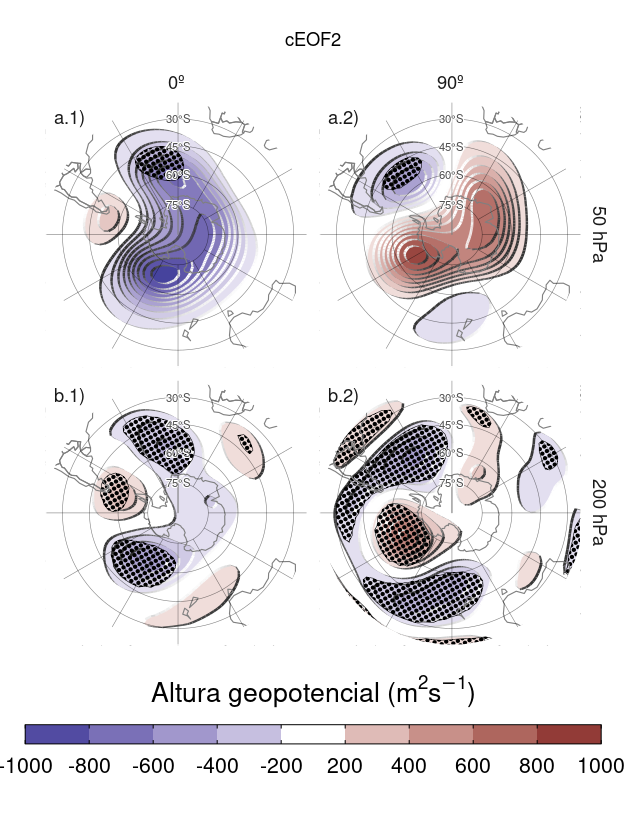
\includegraphics{figures/20-ceofs/eof2-regr-gh-1} 

}

\caption{Igual que la Figura \ref{fig:eof1-regr-gh} pero para el cEOF2.}\label{fig:eof2-regr-gh}
\end{figure}

La Figura \ref{fig:eof2-regr-gh} muestra los mapas de regresión de las anomalías de altura geopotencial para el cEOF2.
Tanto en 50 como en 200 hPa se observan patrones similares a los de la Figura \ref{fig:ceofs-1} columna 2.
Las anomalías de regresión asociadas con la fase de 0º del cEOF2 están desfasadas 1/4 de longitud de onda con respecto a las asociadas con la fase de 90º.
Todos los campos tienen una onda zonal dominante 3 limitada al hemisferio occidental, sobre los océanos Pacífico y Atlántico.

En 50 hPa (Fig. \ref{fig:eof2-regr-gh} fila a) también se destaca un monopolo sobre el polo con signo negativo en la fase de 0º y signo positivo en la fase de 90º.
Este monopolo podría indicar fortalecimiento del vórtice polar asociado a valores positivos de la fase de 0º del cEOF2 y debilitamiento asociado a valores negativos de la fase de 0º del cEOF2.
Sin embargo, estas anomalías no son estadísticamente significativas, indicando que su magnitud es baja en comparación a la variabilidad estratosférica y que esta característica no debe sobreinterpretarse.

En 200 hPa (Fig. \ref{fig:eof2-regr-gh} fila b) el tren de ondas es robusto ya que los centros son estadísticamente significativos, con anomalías insignificantes por fuera de este patrón.
La localización de las anomalías no varía en la vertical, lo cual vuelve a confirmar que se trata de un modo barotrópico equivalente.

El cEOF2 representa entonces un tren de ondas de estructura barotrópica equivalente muy similar al de los patrones PSA (\protect\hyperlink{ref-mo2001}{Mo and Paegle, 2001}).
Comparando la localización de la anomalía positiva cerca de 90ºO en la columna 2 de la Figura \ref{fig:eof2-regr-gh} con las Figuras 1.a y b de Mo and Paegle (\protect\hyperlink{ref-mo2001}{2001}), el mapa de regresión de la fase de 0º podría identificarse con el PSA2, mientras que la fase 90º se asemeja al PSA1.
Por otro lado, ambos modos muestran relación con patrones anulares semejantes al SAM.
Se estudiará la relación entre los cEOF y el PSA con más detalle en la sección \ref{psa}.

\hypertarget{temperatura-y-ozono}{%
\subsubsection{Temperatura y Ozono}\label{temperatura-y-ozono}}



\begin{figure}

{\centering 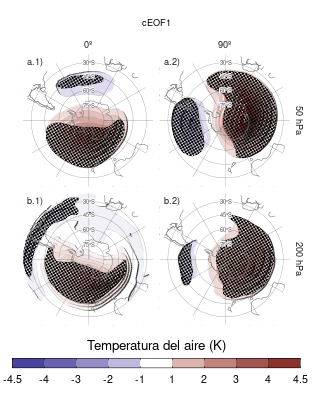
\includegraphics{figures/20-ceofs/eof1-regr-t-1} 

}

\caption{Igual que la Figura~\ref{fig:eof1-regr-gh} pero para la temperatura del aire (K).}\label{fig:eof1-regr-t}
\end{figure}



\begin{figure}

{\centering 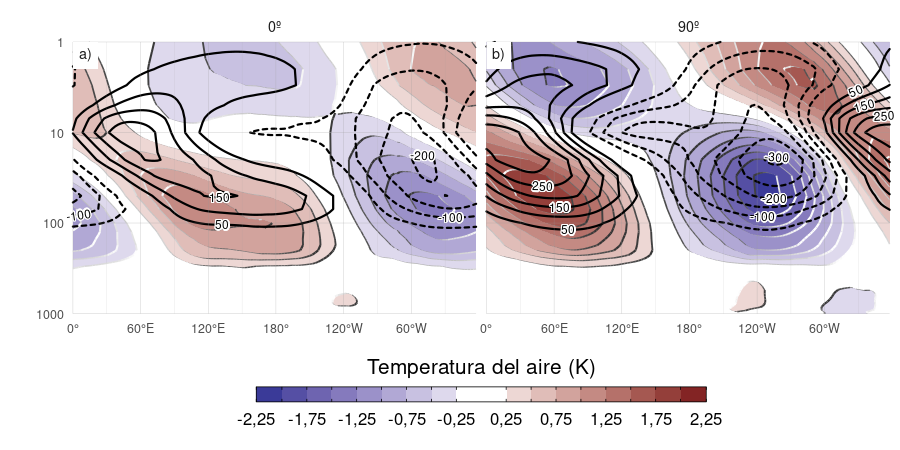
\includegraphics{figures/20-ceofs/t-vertical-1} 

}

\caption{Regresión de anomalías zonales de temperatura (sombrado, K) y razón de mezcla de ozono (contornos, valores negativos en línea punteada, etiquetas en partes por mil millón en masa) promediados entre 75°S y 45°S en SON con la fase de 0º (a) y de 90º (b) del cEOF1 para el período 1979--2020.}\label{fig:t-vertical}
\end{figure}

Se evaluó la señal de la variabilidad de los cEOF en la temperatura del aire.
La Figura \ref{fig:eof1-regr-t} muestra los mapas de regresión de las anomalías de esta variable en 50 hPa y 200 hPa con el cEOF1.
La distribución de los coeficientes de regresión de la temperatura en 50 hPa y en 200 hPa refleja la que muestran los mapas de regresión de la altura geopotencial en 50 hPa (Fig. \ref{fig:eof1-regr-gh}).
Es decir, anomalías positivas de ambas variables ubicadas en las mismas regiones, lo que es indicio del carácter dinámico de los procesos que las vinculan.
En ambos niveles, la fase de 0º está asociada con anomalías positivas sobre el Polo Sur con su centro desplazado ligeramente hacia 150ºE (Fig. \ref{fig:eof1-regr-t} columna 1).
Por otro lado, los mapas de regresión de las anomalías de temperatura con la fase de 90º muestran un patrón de onda 1 más claro con su máximo alrededor de los 60ºE.

La Figura \ref{fig:t-vertical} muestra la distribución vertical de los coeficientes de regresión del cEOF1 con las anomalías zonales de la temperatura del aire y de la razón de mezcla de ozono, ambas promediadas entre 75°S y 45°S.
Las anomalías zonales de temperatura asociadas al cEOF1 muestran un claro patrón de onda 1 tanto para la fase de 0º como para la de 90º en toda la atmósfera por encima de 250 hPa con una inversión de signo por encima de 10 hPa.
Como resultado del balance hidrostático, este es el nivel en el que la anomalía geopotencial tiene máxima amplitud (no se muestra).

Los valores máximos de la regresión con el ozono coinciden con los valores mínimos de temperatura por encima de 10 hPa y con los máximos por debajo de 10 hPa (Fig. \ref{fig:t-vertical}).
Por lo tanto, la onda zonal 1 de ozono está correlacionada negativamente con la onda zonal 1 de temperatura en la estratosfera superior, y positivamente en la estratosfera baja.
Este cambio de fase es típicamente observado en las anomalías de ozono forzadas por ondas planetarias que alcanzan la estratosfera.
En la estratosfera superior, dominada por procesos fotoquímicos, las temperaturas frías inhiben la destrucción de ozono, explicando el comportamiento opuesto para ambas variables, tal y como se dilucidó con modelos químicos dinámicos (\protect\hyperlink{ref-hartmann1979}{Hartmann and Garcia, 1979}; \protect\hyperlink{ref-smith1995}{Smith, 1995}; \protect\hyperlink{ref-wirth1993}{Wirth, 1993}).
Por otro lado, en la estratosfera baja, dominada por la advección, las anomalías de ozono están desfasadas 1/4 de longitud de onda con el transporte horizontal y vertical, que a su vez están desfasados 1/4 de longitud de onda con las anomalías de temperatura, resultando anomalías del mismo signo para la respuesta de ambas variables (\protect\hyperlink{ref-hartmann1979}{Hartmann and Garcia, 1979}; \protect\hyperlink{ref-smith1995}{Smith, 1995}; \protect\hyperlink{ref-wirth1993}{Wirth, 1993}).



\begin{figure}

{\centering 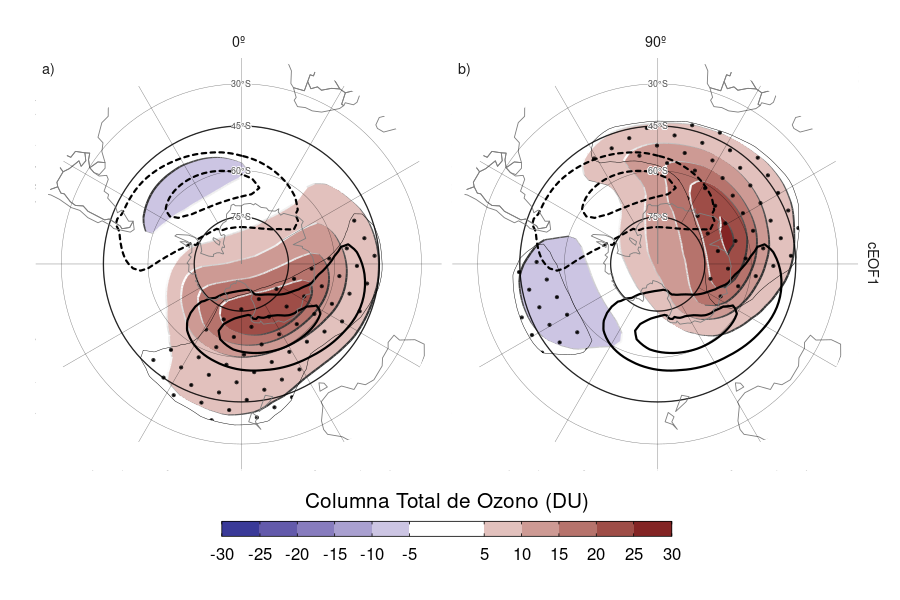
\includegraphics{figures/20-ceofs/o3-regr-1} 

}

\caption{Regresión de las anomalías de Columna Total de Ozono (CTO, sombreado, unidades Dobson) con la fase de 0º (a) y de 90º (b) del cEOF1 para el período 1979--2020. En contornos, la anomalía zonal media de de CTO (contornos negativos en líneas punteadas, unidades Dobson). Áreas con puntos marcan regiones donde el p-valor es menor que 0,01 ajustado por FDR.}\label{fig:o3-regr}
\end{figure}



Los mapas de regresión de las anomalías de CTO con el cEOF1 (Fig. \ref{fig:o3-regr}) muestran patrones de onda zonal 1 en ambas fases del cEOF1.
La posición climatológica del mínimo de ozono durante la primavera no está centrada sobre el Polo Sur, sino que está desplazada hacia el mar de Weddell (ej, \protect\hyperlink{ref-grytsai2011}{Grytsai, 2011}); este desplazamiento se traduce en una onda 1 de la CTO.
Así, el campo de regresión de la fase de 0º del cEOF1 (Fig.~\ref{fig:o3-regr}a) coincide con la posición climatológica de esta onda 1 del mínimo de ozono, mientras que el campo para la fase de 90º está defasado en 90º cEOF1.
La correlación temporal entre la amplitud de la onda 1 de CTO y la amplitud del cEOF1 es 0,79 (CI: 0,63 -- 0,88), mientras que la correlación entre sus fases es -0,85 (CI: -0,92 -- -0,74).
La correlación entre las dos ondas es -0,87 (CI: -0,93 -- -0,77).
Esto implica que el cEOF1 está fuertemente relacionado con la variabilidad del ozono del hemisferio sur.

\hypertarget{psa}{%
\subsection{PSA}\label{psa}}



\begin{table}

\caption{\label{tab:psa-eof2}Coeficiente de correlación entre las series temporales de las fases de 0º y 90º del cEOF2 con los modos PSA1 y PSA2 para el período 1979--2020. Los intervalos de confianza de 95\% se muestran en paréntesis. Estimaciones significativas con p-valor menor a 0,01 en negrita.}
\centering
\begin{tabular}[t]{l>{}l>{}l}
\toprule
PC & 0º & 90º\\
\midrule
PSA1 & 0,15 (CI: -0,16 -- 0,44) & \textbf{0,74 (CI: 0,56 -- 0,85)}\\
\cmidrule{1-3}
PSA2 & \textbf{0,77 (CI: 0,61 -- 0,87)} & 0,25 (CI: -0,06 -- 0,52)\\
\bottomrule
\end{tabular}
\end{table}

Dada la similitud entre las estructuras asociadas al cEOF2 (Fig. \ref{fig:eof2-regr-gh}) y los patrones del PSA, se estudió la relación entre ellos con mayor profundidad.
La Tabla \ref{tab:psa-eof2} muestra las correlaciones entre las series temporales del PSA1 y el PSA2 y las series temporales de las fases de 0º y 90º del cEOF2.
Como se anticipaba visualmente en la Figura \ref{fig:eof2-regr-gh}, existen correlaciones positivas altas entre el PSA1 y la fase de 90º, y entre el PSA2 y la fase de 0º cEOF2.
Por otro lado, no existe una relación significativa entre el PSA1 y la fase de 0º ni entre el PSA2 y la fase de 90º cEOF2.
En consecuencia, el cEOF2 representa bien tanto la estructura espacial como la evolución temporal de los modos PSA, por lo que es posible establecer una asociación entre sus dos fases y los dos modos PSA.
Es decir, la fase del cEOF2 que tiene máxima correlación con el ENSO es la que tiene máxima correlación con el PSA1 y la fase del cEOF2 que tiene mínima correlación con el ENSO es la que tiene máxima correlación con el PSA2 (no se muestra).



\begin{figure}

{\centering 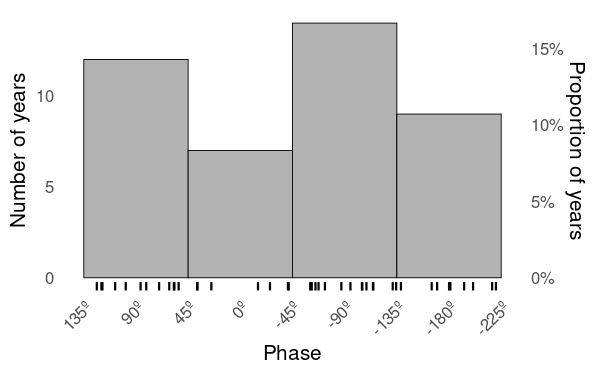
\includegraphics{figures/20-ceofs/phase-histogram-1} 

}

\caption{Histograma de la distribución de fases del cEOF2 para el periodo 1979--2020. Los intervalos están centrados en 90º, 0º, -90º, -180º con un ancho del intervalo de 90º. Las pequeñas líneas verticales cerca del eje horizontal marcan los valores de cada trimestre SON.}\label{fig:phase-histogram}
\end{figure}

La Figura \ref{fig:phase-histogram} muestra un histograma para cada trimestre con la distribución de la fase del cEOF2, donde se marcan también las observaciones con líneas verticales en el eje horizontal.
El cEOF2 tiene una fase similar a \(\pm\) 90º en un 62\% de los años, indicando que es la fase más común.
Esta preferencia de fase está de acuerdo con Irving and Simmonds (\protect\hyperlink{ref-irving2016}{2016}) que encontró una distribución bimodal en la variabilidad tipo PSA (comparación de la Figura \ref{fig:phase-histogram} con la Figura 6 de Irving and Simmonds (\protect\hyperlink{ref-irving2016}{2016})).

Estos resultados sugieren entonces que el cEOF2 permite caracterizar la variabilidad del PSA de forma alternativa al EOF tradicional propuesto por Mo and Paegle (\protect\hyperlink{ref-mo2001}{2001}), entre otros autores.
De esta forma, con la metodología de cEOF se puede caracterizar al PSA como un continuo de ubicaciones, en vez de como dos modos estacionarios separados, como surge de la metodología de EOF.

\hypertarget{fuentes-ceof}{%
\subsection{Fuentes de variabilidad tropical}\label{fuentes-ceof}}



\begin{figure}

{\centering 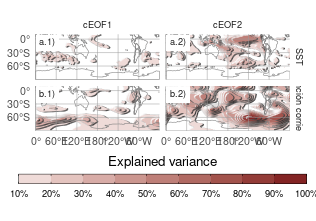
\includegraphics{figures/20-ceofs/psi-sst-explained-variance-1} 

}

\caption{Porcentaje de varianza de las anomalías de TSM (fila a) y de las anomalías zonales de función corriente (fila b) explicada por el cEOF1 (columna 1) el cEOF2 (columna 2).}\label{fig:psi-sst-explained-variance}
\end{figure}

Para evaluar si la variabilidad de los cEOF analizados está relacionada con fuentes de variabilidad en la banda tropical se calculó la regresión de distintas fases de los cEOFs con las anomalías de TSM y con las anomalías zonales de función corriente en 200 hPa.
La Figura \ref{fig:psi-sst-explained-variance} muestra la varianza de cada variable explicada por cada cEOF a partir de la regresión lineal múltiple de ambas fases.

El cEOF2, en cambio, se asocia con una gran proporción de la variabilidad tropical tanto de las anomalías de TSM como de las de función corriente (Fig. \ref{fig:psi-sst-explained-variance} columna 2).
Este modo comparte más de un 50\% de la varianza con las TSM en el Pacífico central , sugiriendo la influencia del ENSO.
En cuanto a la función corriente, en el Pacífico el modo explica más del 50\% de la varianza en la región del cambio de fecha y sobre Indonesia.
También explica gran parte de la varianza en al oeste y al este de la Península Antártica, llegando a más del 80\% sobre el mar de Amundsen.



\begin{figure}

{\centering 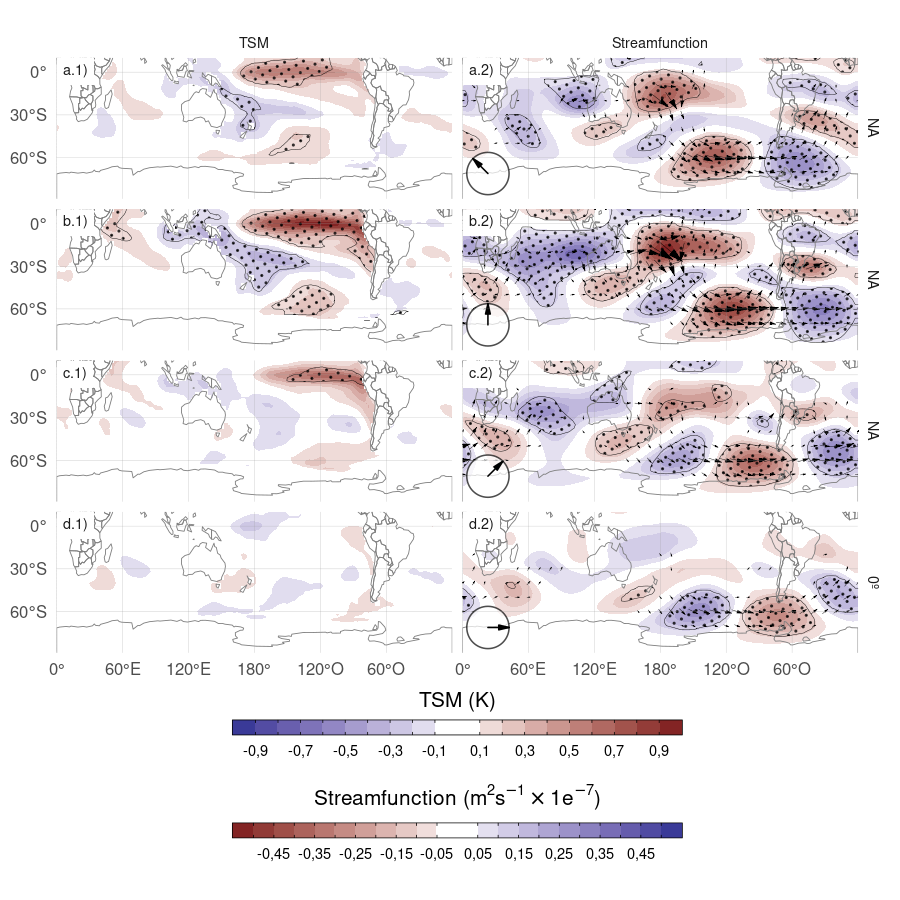
\includegraphics{figures/20-ceofs/sst-psi-2-1} 

}

\caption{Regresión de (columna 1) TSM (K) y (columna 2) anomalías zonales de función corriente (\(m^2/s\times10^-7\)) y sus vectores de acción de onda con diferentes fases del cEOF2 (indicado con la flecha) en el período 1979--2020. Áreas con puntos marcan regiones donde el p-valor es menor que 0,01 ajustado por FDR.}\label{fig:sst-psi-2}
\end{figure}

La Figura \ref{fig:sst-psi-2} muestra los mapas de regresión de las anomalías de la temperatura de la superficie del mar (TSM) y de la función de corriente a 200 hPa con las series temporales normalizadas de cada fase del cEOF2.
Además de los mapas de regresión para las fases de 0º y 90º, se incluyen las regresiones correspondientes para dos fases intermedias (correspondientes a 45º y 135º).
Para esto, se rotaron los cEOF en 1/4 de longitud de onda multiplicando las series temporales complejas por \(cos(\pi/4) + i\sin(\pi/4)\) y calculando la regresión sobre esas series temporales rotadas.

La fase de 90º (Fig. \ref{fig:sst-psi-2} fila b) está asociada a fuertes anomalías positivas de la TSM en el Pacífico central y oriental y a anomalías negativas en una zona que atraviesa el norte de Australia, Nueva Zelanda y la Zona de Convergencia del Pacífico Sur (SPCZ) (Fig. \ref{fig:sst-psi-2}.b1).
Este patrón es muy similar al patrón del ENSO positivo canónico (\protect\hyperlink{ref-bamston1997}{Bamston et al., 1997}).
De hecho, existe una correlación significativa y muy alta entre el ONI y la serie temporal de la fase de 90º del cEOF2 (0,76 (CI: 0,6 -- 0,87)).
Además del patrón similar al ENSO del Pacífico, también hay anomalías positivas en el océano Índico occidental y valores negativos en el océano Índico oriental, lo que se asemeja al patrón DMI en su fase positiva (\protect\hyperlink{ref-saji1999}{Saji et al., 1999}).
Consistentemente, la correlación entre la fase de 90º del cEOF2 y el DMI es 0,62 (CI: 0,38 -- 0,77).
Sin embargo, la correlación semiparcial es de 0,21 (p-valor = 0,18), indicando que el DMI explica poca varianza de la fase de 90º del cEOF2 por sí mismo.
Esto puede observarse en la Figura \ref{fig:euler}, donde se ilustra la partición de la varianza de la fase de 90º del cEOF2, el DMI y el ONI.
El DMI explica, independientemente, sólo un 4.5\% de la varianza, mientras que el ONI explica un 24.8\% por sí mismo.

\begin{figure}

{\centering 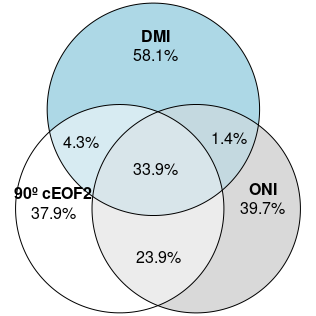
\includegraphics{figures/20-ceofs/euler-1} 

}

\caption{Diagrama de Euler mostrando la proporción de la varianza de cada serie (DMI, ONI y la fase de 90º del cEOF2) explicada por las demás (p.ej. la región común entre DMI y ONI es la varianza del DMI explicada por el ONI y viceversa).}\label{fig:euler}
\end{figure}



La fase de 90º del cEOF2 está asociada a anomalías de la función corriente que emanan de los trópicos (Fig. \ref{fig:sst-psi-2}.b2), tanto del sector del Pacífico Central como del Océano Índico.
Esta respuesta atmosférica es consistente con el efecto combinado del ENSO y el DMI sobre los extratrópicos: con anomalías de la TSM que inducen convección tropical anómala en ambas cuencas oceánicas, que a su vez excita ondas de Rossby que se propagan meridionalmente hacia latitudes más altas (\protect\hyperlink{ref-cai2011}{Cai et al., 2011}; p.ej. \protect\hyperlink{ref-mo2000}{Mo, 2000}; \protect\hyperlink{ref-nuncio2015}{Nuncio and Yuan, 2015}).

Sin embargo, el cEOF2 no está asociado a los mismos patrones de anomalía de las TSM tropicales en todas sus fases.
Los paneles d1 y d2 de la Figura \ref{fig:sst-psi-2} muestran que la fase de 0º del cEOF2 no está asociada a ninguna anomalía significativa de las TSM ni de la función corriente en los trópicos.
Tampoco la correlación entre la fase de 0º del cEOF2 y el ENSO es significativa (0 (CI: -0,3 -- 0,31)).
Las filas a y c de la Fig.\ref{fig:sst-psi-2} muestran que las fases intermedias siguen asociadas con anomalías significativas de la TSM sobre el Océano Pacífico, pero en lugares ligeramente diferentes.
La fase de 135º está asociada a anomalías de la TSM en el Pacífico central (Fig.\ref{fig:sst-psi-2}a.1), mientras que la fase de 45º (Fig.\ref{fig:sst-psi-2}c.1) está asociada a anomalías de la TSM que corresponden aproximadamente a los ``sabores'' de ENSO del Pacífico central y del Pacífico oriental, respectivamente (\protect\hyperlink{ref-kao2009}{Kao and Yu, 2009}).
Ambas fases también están asociadas a trenes de onda que se generan cerca de Australia y se propagan hacia los extratrópicos, aunque menos intensos que los asociados a la fase de 90º.



\begin{figure}

{\centering 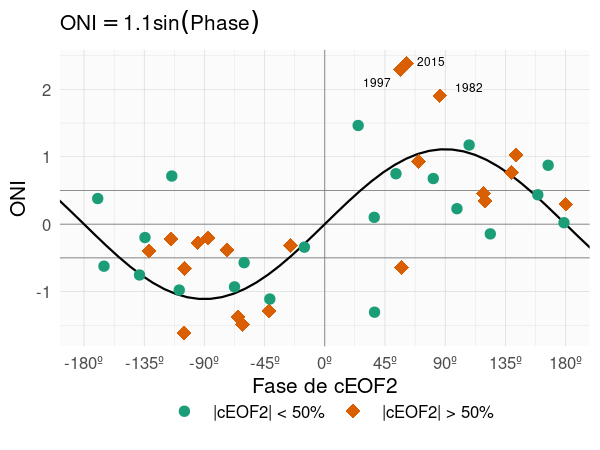
\includegraphics{figures/20-ceofs/enso-phase-1} 

}

\caption{Valores del ONI en SON y la fase del cEOF2 en el período 1979--2020. Los años en los cuales la magnitud del cEOF2 es mayor o menor que la mediana se muestran como diamantes naranja o círculos verdes respectivamente. La línea negra representa el ajuste ONI \textasciitilde{} sen(fase) computado por cuadrados mínimos pesados por la magnitud del cEOF2.}\label{fig:enso-phase}
\end{figure}

Para explorar la relación entre el forzante tropical y las fases del cEOF2 con más profundidad, la Figura \ref{fig:enso-phase} muestra la relación entre los valores del ONI y de la fase del cEOF2 para cada SON entre 1979 y 2020, destacando los años en los que la magnitud del cEOF2 está por encima de la mediana.
En los años con ONI positivo, la fase cEOF2 se sitúa mayoritariamente en torno a la fase de 90º; mientras que en los años con ONI negativo, en torno a la fase de -90º.
Por otra parte, en los años con ENSO neutro, la fase del cEOF2 es mucho más variable.
La línea negra de la Figura \ref{fig:enso-phase} es un ajuste sinusoidal de la relación entre el ONI y la fase del cEOF2.
El \(r^2\) correspondiente al ajuste es 0,57, estadísticamente significativo con p-valor \textless{} 0,001, lo que indica una relación aproximadamente sinusoidal entre estas dos variables.

\begin{figure}

{\centering 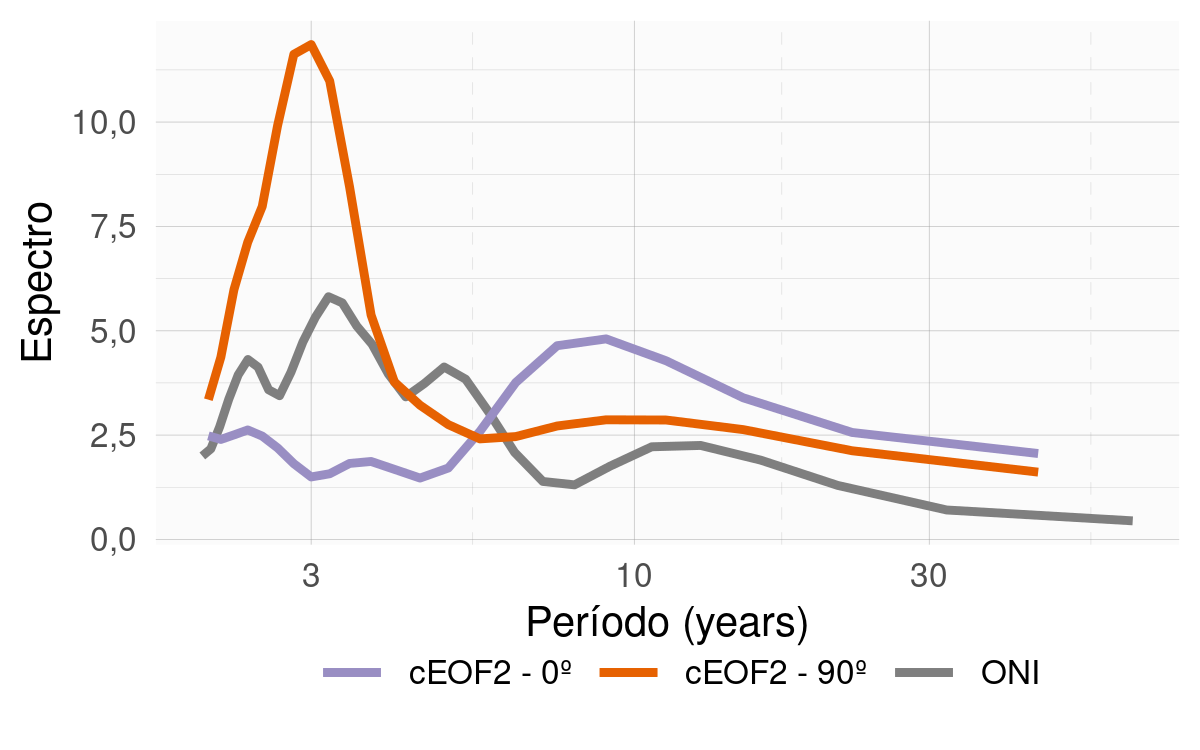
\includegraphics{figures/20-ceofs/fft-ceof-era5-1} 

}

\caption{Espectro de Fourier para cada fase de 0º del cEOF2 (línea azul), fase de 90º del cEOF2 (línea naranja) y el ONI (línea gris).}\label{fig:fft-ceof-era5}
\end{figure}



Otra evidencia de la relación entre el ENSO y la fase del cEOF2 es que tanto el ONI como la fase de 90º del cEOF2 tienen un pico de periodicidad alrededor de 3 años (Fig. \ref{fig:fft-ceof-era5}.
Esto muestra que la principal escala de variabilidad de esta fase está íntimamente relacionada con el ENSO.

La correlación entre la magnitud absoluta del ONI y la amplitud del cEOF2 es 0,45 (CI: 0,17 -- 0,66).
Sin embargo, esta relación está determinada principalmente por los tres años con los eventos ENSO más intensos del periodo (2015, 1997, y 1982), los cuales coinciden con los tres años con la magnitud del cEOF2 más grande (no se muestra).
Si se eliminan esos años, la correlación deja de ser significativa (0,04 (CI: -0,28 -- 0,35)).
Además, incluso utilizando todos los años, la correlación de Spearman -que es robusta frente a los valores atípicos- tampoco es significativa (0,2, p-valor = 0,21).
Por lo tanto, aunque la localización de las anomalías tropicales de la TSM parece tener un efecto en la definición de la fase del cEOF2, la relación entre la magnitud del cEOF2 y el ONI sigue siendo incierta y podría ser sólo evidente en eventos ENSO muy fuertes, que son escasos en el registro observacional histórico.

Se puede concluir que el tren de ondas representado por el cEOF2 está asociado tanto con la variabilidad interna de la atmósfera como forzado por las TSM tropicales.
En el primer caso, el tren de ondas tiene poca preferencia de fase.
Sin embargo, cuando el cEOF2 es excitado por la variabilidad de la TSM tropical, tiende a permanecer fijo en la fase de 90º.



\begin{figure}

{\centering 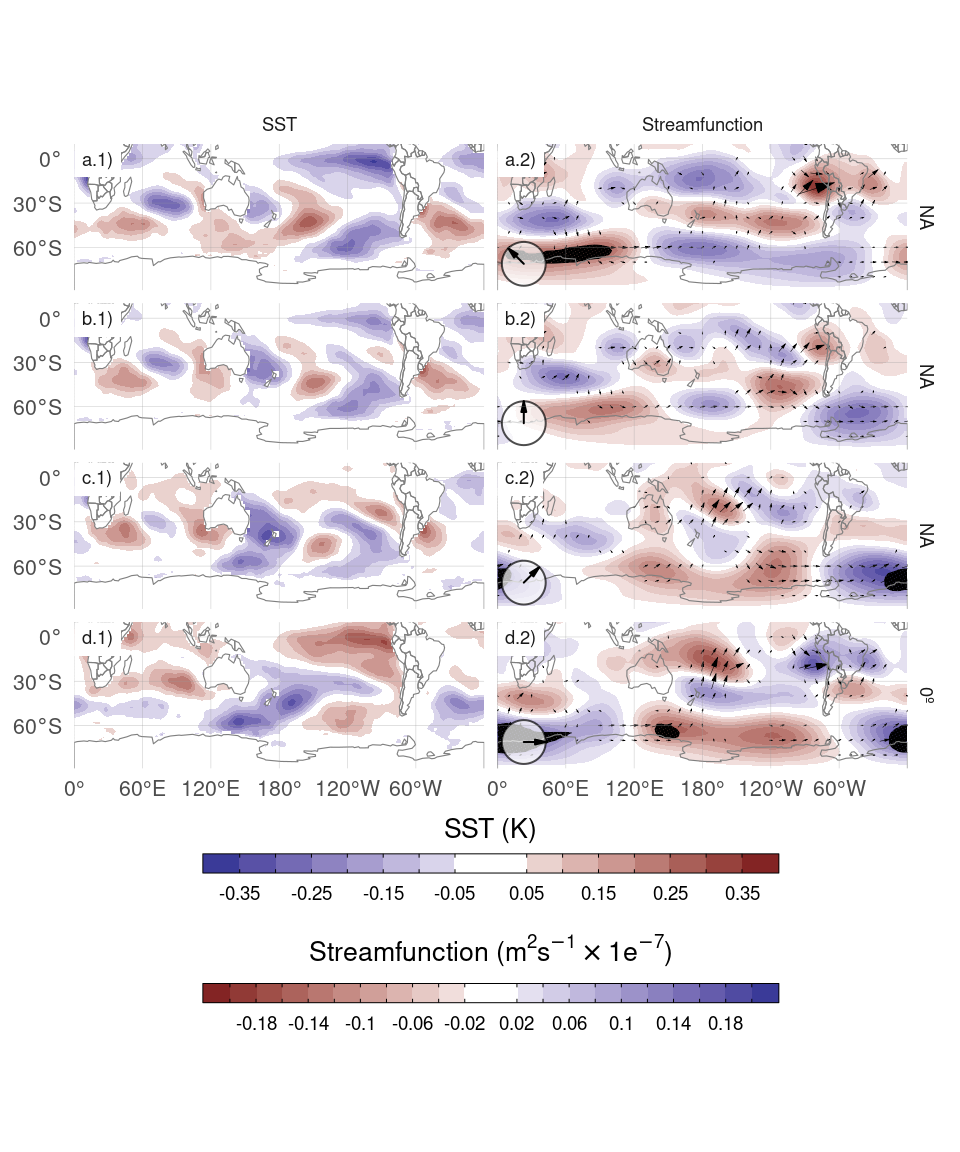
\includegraphics{figures/20-ceofs/sst-psi-1-1} 

}

\caption{Igual que la Figura~\ref{fig:sst-psi-2} pero para el cEOF1.}\label{fig:sst-psi-1}
\end{figure}

La Figura \ref{fig:sst-psi-1} muestra las mismas regresiones que la Figura \ref{fig:sst-psi-2} pero para el cEOF1.
Como anticipó la Figura \ref{fig:psi-sst-explained-variance}, el cEOF1 no está asociado con anomalías significativas de TSM ni de función corriente en los trópicos.
En vez de eso, las fases de 0º y 90º están asociadas a flujos de actividad de onda que se propagan zonalmente en los extratrópicos cerca de de 60ºS, excepto por un flujo hacia el ecuador desde la costa de la Antártida alrededor de 150ºE en la fase de 0º.
Esto sugiere que la variabilidad de cEOF1 está impulsada principalmente por la variabilidad interna de las latitudes medias y altas.

\hypertarget{impactos}{%
\subsection{Impactos en superficie}\label{impactos}}

\begin{figure}

{\centering 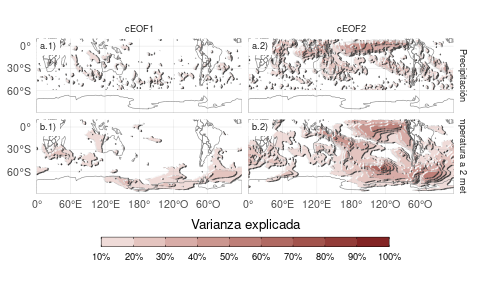
\includegraphics{figures/20-ceofs/pp-t2m-r2-1} 

}

\caption{Igual que la Figura \ref{fig:psi-sst-explained-variance} pero para Temperatura a 2 metros y precipitación.}\label{fig:pp-t2m-r2}
\end{figure}



Teniendo en cuenta el impacto que producen regionalmente tanto las variaciones de la temperatura cerca de superficie como la precipitación, en esta sección se explora la influencia de los modos cEOF sobre estas dos variables.
La Figura \ref{fig:pp-t2m-r2} muestra la varianza de la temperatura del aire a 2 metros y de la precipitación explicada por cada cEOF.

La varianza explicada por el cEOF1 para ambas variables es muy baja en la mayoría de las regiones, excepto para el extremo norte de la Península Antártica, el norte del Mar de Weddell y la costa del Mar de Ross (Fig.\ref{fig:pp-t2m-r2}a.1).
Por otro lado, la varianza explicada por el cEOF2 es superior al 50\% en algunas regiones para ambas variables (Fig. \ref{fig:pp-t2m-r2} columna 2).
Para la temperatura del aire a 2 metros, hay valores altos en el Pacífico tropical y en la región que forma un arco entre Nueva Zelanda y el Atlántico Sur.
Sobre los continentes, hay valores moderados de alrededor del 30\% de varianza explicada en el sur de Australia, el sur de Sudamérica y la Península Antártica.
En cuanto a las precipitaciones, los valores asociados con este modo son elevados en los trópicos.
En latitudes más altas, se observan valores moderados sobre el este de Australia y algunas regiones del sur de Sudamérica.

Dado que el cEOF1 tiene una señal relativamente débil en las variables de superficie exploradas, se analizó con mayor profundidad la influencia del cEOF2 sobre estas dos variables.
En la Figura \ref{fig:pp-temp-2} se muestran los mapas de regresión de las anomalías de precipitación (columna 1) y de temperatura del aire a 2 metros (columna 2) para diferentes fases del cEOF2 normalizado.



\begin{figure}

{\centering 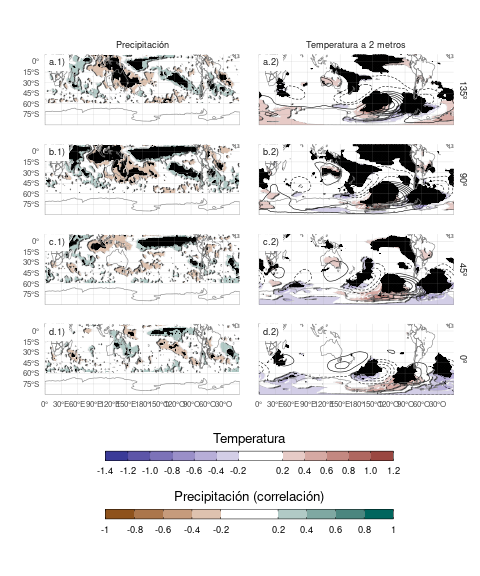
\includegraphics{figures/20-ceofs/pp-temp-2-1} 

}

\caption{Regresión de la precipitación (correlación, columna 1) y la temperatura de 2 metros (K, sombreado) y la altura geopotencial de 850 hPa (m, contornos, columna 2) sobre diferentes fases de cEOF2 para el trimestre SON del periodo 1979--2020. Áreas con puntos marcan regiones donde el p-valor es menor que 0,01 ajustado por FDR.}\label{fig:pp-temp-2}
\end{figure}

Las anomalías de temperatura asociadas a la fase de 90º del cEOF2 (Fig.~\ref{fig:pp-temp-2}b.2) muestran valores positivos en el Pacífico tropical, coherentes con las anomalías de TSM asociadas a esta misma fase (Fig.~\ref{fig:sst-psi-2}b.1).
En latitudes más altas existe un patrón oscilatorio de valores positivos y negativos alternados que coincide con los nodos de los patrones de regresión de la altura geopotencial de 850 hPa.
Esto es coherente con las anomalías de temperatura producidas dinámicamente por la advección de temperatura por los vientos meridionales derivados del equilibrio geostrófico.
Sobre los continentes, las fase de 90º (Fig.\ref{fig:pp-temp-2}b.2) está asociada con anomalías de temperatura positiva en el sur de Australia y anomalías de regresión negativa en el sur de Sudamérica y la Península Antártica, que son resultado del tren de ondas descrito anteriormente.

Las anomalías de temperatura asociadas a la fase de 0º (Fig.\ref{fig:pp-temp-2}d.2) son menos extensas y se limitan a latitudes medias y altas.
Sobre los continentes, las regresiones de las anomalías de temperatura no son significativas, excepto las anomalías positivas cerca de la Península Antártica.

Las anomalías de precipitación tropicales asociadas a la fase de 90º del cEOF2 son importantes, con anomalías positivas en el Pacífico central y el Índico occidental, y anomalías negativas en el Pacífico oriental (Fig.\ref{fig:pp-temp-2}b.1).
Este campo es consistente con el mapa de regresión de la TSM (Fig.\ref{fig:sst-psi-2}b.1), ya que las anomalías positivas de la TSM potencian la convección tropical y las anomalías negativas de la TSM la inhiben.

En los extratrópicos, la fase de 90º del cEOF2 se asocia a condiciones más secas sobre el este de Australia y el océano circundante, que es una señal similar a la asociada al ENSO (\protect\hyperlink{ref-cai2011}{Cai et al., 2011}).
Sin embargo, esta es la fase más fuertemente correlacionada con la precipitación en esa zona.
La fase de 135º (una intermedia 90º y 180º) está correlacionada más intensa y extensamente con la precipitación sobre Australia y Nueva Zelanda.
La influencia del cEOF2 en la precipitación australiana podría estar relacionada más con los impactos directos de las anomalías de la TSM en los océanos circundantes que en el patrón de teleconexión representado por el cEOF2.

Sobre Sudamérica, la fase de 90º del cEOF2 está correlacionada positivamente con la precipitación en el SESA y el centro de Chile, y negativamente en el este de Brasil.
Este campo de correlación es coherente con la señal de ENSO en la precipitación regional de primavera (p.ej. \protect\hyperlink{ref-cai2020a}{Cai et al., 2020}).

Los coeficientes de correlación entre las anomalías de precipitación y la fase de 0º del cEOF2 (Fig.~\ref{fig:pp-temp-2}d.2) son más débiles que para la fase de 90º.
Hay una correlación positiva residual en el Pacífico oriental ecuatorial y pequeñas correlaciones positivas, que son son estadísticamente significativas, sobre el este de Australia y negativas sobre Nueva Zelanda.

\hypertarget{conclusiones-del-capuxedtulo-refceofs}{%
\section{Conclusiones del capítulo \ref{ceofs}}\label{conclusiones-del-capuxedtulo-refceofs}}

Los cEOF identificados a partir de las anomalias zonales de altura geopotencial en 50 y 200 hPa conjuntamente logran representar características importantes de la circulación zonalmente asimétrica del hemisferio sur.
El cEOF1 captura principalmente la estructura espacio-temporal de la onda 1 en la estratósfera mientras que el cEOF2 representa la variabilidad de la onda 3 con máxima actividad en la troposfera y latitudes medias pero con un máximo de amplitud en el Pacífico sur.

El cEOF2 está asociado a forzantes tropicales y los trenes de ondas que representa se asemeja a los modos PSA y a la señal del ENSO en la circulación del hemisferio sur.
Por otra parte, las anomalías de circulación asociada a ambos cEOF tiene también características similares al SAM.
Antes de estudiar estas relación en más detalle, se decidió estudiar el SAM y entender mejor sus características zonalmente simétricas y asimétricas.

Los principales resultados de este capítulo han sido publicados en Campitelli et al. (\protect\hyperlink{ref-campitelli2023}{2023}).

\hypertarget{asymsam}{%
\chapter{Estructura simétrica y asimétrica del SAM}\label{asymsam}}

\hypertarget{introducciuxf3n-1}{%
\section{Introducción}\label{introducciuxf3n-1}}

Como se explicó en la introducción, el patrón espacial del SAM suele describirse a través del primer EOF de las anomalías de altura geopotencial en la troposfera del hemisferio sur.
En otros casos se utilizan índices construidos asumiendo que el patrón describe eminentemente variaciones de la circulación zonalmente simétrica.
Sin embargo, este patrón tiene asimetrías zonales significativas.

Muchos índices presentados en la literatura para describir el SAM se basan en medias zonales de la presión a nivel del mar o de la altura geopotencial (\protect\hyperlink{ref-ho2012}{Ho et al., 2012}).
Tanto Gong and Wang (\protect\hyperlink{ref-gong1999}{1999}) como Marshall (\protect\hyperlink{ref-marshall2003}{2003}) definen el índice SAM como la diferencia de la media zonal de la presión a nivel del mar entre 40ºS y 65ºS.
Asimismo,Baldwin and Thompson (\protect\hyperlink{ref-baldwin2009}{2009}) propuso definir modos anulares del norte y el sur como el primer EOF de la altura geopotencial promediada zonalmente en cada nivel en cada hemisferio.
Sin embargo, como se verá a continuación, las asimetrías zonales del SAM pueden ser significativas y han sido poco estudiadas.

En la literatura se asocia generalmente a la fase positiva del SAM a aquella asociada con anomalías negativas de altura geopotencial sobre la Antártida y positivas en latitudes medias (\protect\hyperlink{ref-jones2019}{M. E. Jones et al., 2019}).
En esta fase las temperaturas son más frías de lo normal sobre la Antártida y más cálidas de lo normal en latitudes más bajas.
Lo opuesto se encuentra para la fase negativa.
Pero hay desviaciones significativas de esta respuesta media zonal, especialmente en la Península Antártica y el Atlántico sur (\protect\hyperlink{ref-fogt2012}{Fogt et al., 2012}).
La señal relacionada con el SAM en las anomalías de precipitación también es positiva en latitudes altas y negativa en latitudes medias, aunque con aún mayores desviaciones respecto de la simetría zonal (\protect\hyperlink{ref-lim2016}{Lim et al., 2016}).
En particular, la relación entre el SAM y la precipitación en el SESA~en escalas interanuales depende fuertemente de las anomalías de circulación zonalmente asimétrica asociadas al SAM y presenta importantes variaciones decadales (\protect\hyperlink{ref-rosso2018}{Rosso et al., 2018}; \protect\hyperlink{ref-silvestri2009}{Silvestri and Vera, 2009}).

Si bien la variabilidad del SAM se debe principalmente a la variabilidad interna, en escalas intraestacionales e interanuales, puede estar asociada con la variabilidad tropical (\protect\hyperlink{ref-clem2013}{Clem and Fogt, 2013}; \protect\hyperlink{ref-fan2007}{Fan, 2007}; \protect\hyperlink{ref-fogt2011a}{Fogt et al., 2011}).
Como se discutió en las secciones anteriores, el ENSO o la variabilidad tropical en general afecta a los extratrópicos del hemisferio sur a través de trenes de ondas de Rossby (\protect\hyperlink{ref-karoly1989}{Karoly, 1989}; \protect\hyperlink{ref-kidson1988}{Kidson, 1988}; \protect\hyperlink{ref-mo1987}{Mo and Ghil, 1987}) que pueden proyectarse fuertemente sobre las anomalías zonales asociadas al SAM en el sector del Pacífico (p.ej. \protect\hyperlink{ref-silvestri2009}{Silvestri and Vera, 2009}; \protect\hyperlink{ref-vera2018}{Vera and Osman, 2018}).
Fan (\protect\hyperlink{ref-fan2007}{2007}) calculó los índices de SAM de los hemisferios occidental y oriental por separado y encontró que la correlación entre ellos aumentaba si se elimina la señal (lineal) del ENSO, sugiriendo que la influencia del ENSO en el SAM no es zonalmente homogénea.

En escalas más largas, investigaciones previas han documentado a lo largo del siglo XX y lo que va del XXI, tendencias positivas en el SAM utilizando diferentes índices, sobre todo para el verano y otoño australes (p.ej., \protect\hyperlink{ref-fogt2020}{Fogt and Marshall, 2020} y sus referencias).
Se encontró que estas tendencias están impulsadas principalmente por la reducción del ozono estratosférico y el aumento de los gases de efecto invernadero, aunque han sido analizadas en el contexto de las variables medias zonales (\protect\hyperlink{ref-arblaster2006}{Arblaster and Meehl, 2006}; \protect\hyperlink{ref-gillett2005}{Gillett et al., 2005}; \protect\hyperlink{ref-gillett2013}{Gillett et al., 2013}; \protect\hyperlink{ref-marshall2004}{Marshall et al., 2004}).
Por lo tanto, no está claro si la componente asimétrica del SAM responde a estos forzantes de la misma forma o si su variabilidad, por el contrario, altera las tendencias observadas.

Uno de los pocos trabajos que estudiaron la variabilidad temporal de la componente asimétrica del SAM es Fogt et al. (\protect\hyperlink{ref-fogt2012}{2012}).
Este trabajo definió los patrones de SAM asimétrico positivo y negativo como las anomalías zonales de composiciones de presión al nivel del mar para eventos SAM positivos y negativos.
Sin embargo, estas composiciones se basan en un número reducido de casos y distribuidos inhomogéneamente entre años con y sin información satelital.
Esto es especialmente relevante debido a las inhomogeneidades en los productos de reanálisis anteriores a la era satelital y al posible cambio en la estructura asimétrica del SAM (\protect\hyperlink{ref-silvestri2009}{Silvestri and Vera, 2009}).
Además, Fogt et al. (\protect\hyperlink{ref-fogt2012}{2012}) estudió la componente asimétrica zonal del SAM solamente en la presión a nivel del mar.
Si bien las asimetrías zonales en el patrón espacial del SAM son barotrópicas equivalentes en toda la troposfera, su estructura cambia drásticamente en la estratosfera (\protect\hyperlink{ref-baldwin2009}{Baldwin and Thompson, 2009}).

Es decir, las investigaciones previas sugieren fuertemente que la componente zonalmente asimétrica del SAM puede tener un comportamiento potencialmente muy distinto al de la componente zonalmente simétrica, por lo que su estudio merece particular atención.
En este sentido, en el capítulo anterior se encontró que algunas fases de los cEOFs están asociadas con patrones tipo SAM en distintos niveles.
El objetivo de este capítulo es, por tanto, describir las componentes zonalmente asimétricas y simétricas de la variabilidad del SAM y su relación con los cEOFs.
En primer lugar, se propone una metodología que proporciona, para cada nivel, dos índices que pretenden captar de forma independiente la variabilidad de la componente del SAM simétrica y asimétrica, respectivamente.
Luego se los utilizó para describir su estructura vertical y su coherencia, así como su variabilidad temporal y sus tendencias.
A continuación se estudiaron los patrones espaciales asociados a la variabilidad exclusiva de cada índice centrándose en 50 hPa como nivel estratosférico y 700 hPa como nivel troposférico.
Por último, se investigaron las relaciones del SAM a 700 hPa con las anomalías de temperatura y precipitación.

\hypertarget{datos-y-muxe9todos}{%
\section{Datos y métodos}\label{datos-y-muxe9todos}}

\hypertarget{datos-2}{%
\subsection{Datos}\label{datos-2}}

Se utilizan las mismas fuentes de datos que en capítulos anteriores.
En este capítulo se usaron en particular datos de altura geopotencial, temperatura del aire a 2 metros del conjunto de datos ERA5 y precipitación del conjunto de datos CMAP para el período 1979--2020.

\hypertarget{regresiuxf3n-segmentada}{%
\subsection{Regresión segmentada}\label{regresiuxf3n-segmentada}}

Se utilizó la metodología de regresión lineal segmentada para calcular los campos asociados a las fases positivas y negativas del SAM.
Ésta consiste en ajustar un modelo lineal a tramos con continuidad en cada segmento como se ilustra en la Figura \ref{fig:segmentada-ejemplo} con datos sintéticos.

\begin{figure}

{\centering 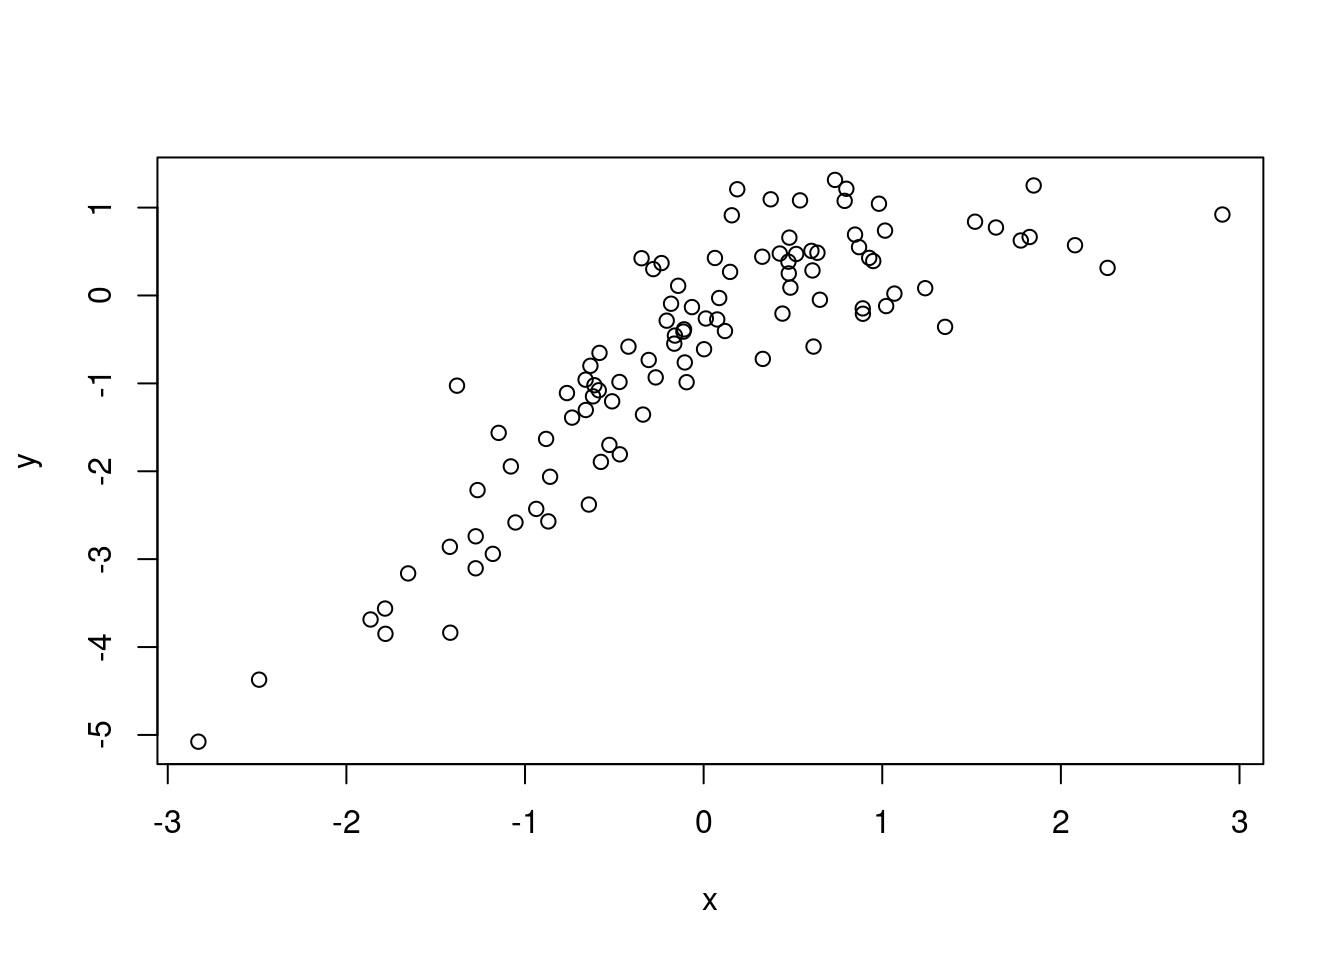
\includegraphics{figures/30-sam/segmentada-ejemplo-1} 

}

\caption{Ejemplo de regresión segmentada. X es una variable aleatoria con distribución uniforme e Y es \(2X\) cuando \(X<0\) y \(1/2X\) cuando \(X\ge0\) más errores aleatorios. La línea azul es la regresión segmentada de X e Y.}\label{fig:segmentada-ejemplo}
\end{figure}



Para obtener las pendientes asociadas a la relación lineal para cada signo, se ajustó la ecuación

\[
Y_i = \alpha X_i + \beta X_iI_{X\le 0} + X_0 + \epsilon_i
\]

donde \(Y\) e \(X\) son las variables dependiente e independiente respectivamente, \(\alpha\) es la pendiente asociada a los valores positivos de \(X\), \(\beta\) es la diferencia entre la pendiente asociada a valores positivos y negativos de \(X\), \(I_{X\le 0}\) es la función indicador que es 1 cuando \(X\le0\) y 0 cuando \(X>0\), y \(X_0\) y \(\epsilon_i\) son la constante y los términos de error.
El coeficiente asociado a valores negativos de X es \(\beta - \alpha\).

Comparado con el uso de composiciones para eventos que superan umbrales positivos y negativos, este método tiene la ventaja de utilizar todos los datos eficientemente (en vez de descartar los eventos ``neutrales'') y de que la magnitud de los patrones obtenidos no depende de la intensidad media de los eventos positivos y negativos.
Además, dado que \(\beta\) es la diferencia en la pendiente entre valores positivos y negativos, es posible calcular la significancia estadística de la misma.

\hypertarget{definition-of-indices}{%
\subsection{Descomposición de las componentes del SAM}\label{definition-of-indices}}

El SAM suele en muchos casos definirse como el EOF de las anomalías de la presión al nivel del mar o de la altura geopotencial en un determinado nivel vertical, generalmente bajo de la troposfera (\protect\hyperlink{ref-ho2012}{Ho et al., 2012}; ej \protect\hyperlink{ref-silvestri2009}{Silvestri and Vera, 2009}).
Siguiendo a Baldwin (\protect\hyperlink{ref-baldwin2001}{2001}), se amplió esa definición verticalmente y se utiliza el término SAM para referirse al primer EOF de las anomalías mensuales de altura geopotencial al sur de 20º S en cada nivel vertical considerado y que de ahora en adelante el SAM se refiere al SAM ``completo'' que incluye tanto la componente simétrica como la asimétrica.

Para separar la componente zonalmente simétrica y la asimétrica del SAM, se calculó la media zonal y las anomalías del patrón espacial del SAM completo, como se muestra en la Figura \ref{fig:method} en 700 hPa.
La señal espacial completa (\(\mathrm{EOF_1}(\lambda, \phi)\)) es la suma de la componente zonalmente asimétrica (\(\mathrm{EOF_1^*}(\lambda, \phi)\)) y la simétrica (\([\mathrm{EOF_1}](\lambda, \phi)\)).
A continuación, se calculó el índice SAM, el índice SAM asimétrico (A-SAM) y el índice SAM simétrico (S-SAM) como los coeficientes de la regresión de cada campo de altura geopotencial mensual sobre los respectivos patrones (ponderando por el coseno de la latitud).
Finalmente, se normalizaron los tres índices dividiéndolos por la desviación estándar del índice SAM en cada nivel.
Como resultado, las magnitudes entre los índices son comparables.
Sin embargo, sólo el índice SAM tiene desviación estándar unitaria por definición.
La varianza explicada por cada patrón se utiliza como indicador del grado de simetría o asimetría zonal de cada campo mensual.
Para cuantificar la coherencia entre las series temporales correspondientes a distintos índices o al mismo índice en distintos niveles, se calculó la correlación temporal entre ellas.



\begin{figure}

{\centering 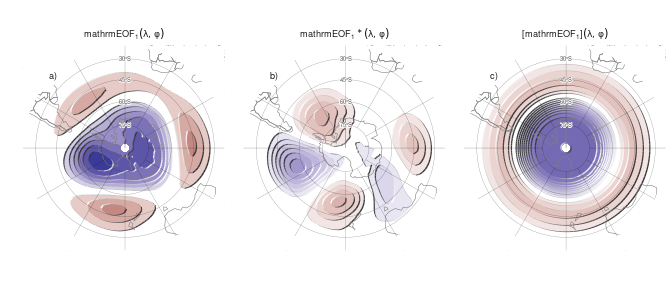
\includegraphics{figures/30-sam/method-1} 

}

\caption{Patrones espaciales del primer EOF de la altura geopotencial en 700 hPa para el período 1979--2020. (a) Campo completo, (b) componente zonalmente asimétrica y (c) componente zonalmente simétrica. Unidades arbitrarias con valores negativos en azul y positivos en rojo.}\label{fig:method}
\end{figure}

Cabe mencionar que una limitación de este método es que supone linealidad en entre las componentes del SAM.
Es decir, supone que los patrones de anomalías asociadas a valores positivos de cada componente del SAM son similares pero de signo opuesto a las asociadas a la fase valores negativos y de magnitud proporcional a la magnitud del índice.
Las composiciones de Fogt et al. (\protect\hyperlink{ref-fogt2012}{2012}) (su Figura 4) sugieren que esto podría no ser del todo válido, aunque gran parte de esa aparente no linealidad podría deberse a la naturaleza heterogénea de los años seleccionados para construir las composiciones y a la incertidumbre muestral.

Para poner esta suposición a prueba, se calculó la regresión segmentada de las anomalías zonales de altura geopotencial con el índice SAM para cada signo del SAM.
Las Figuras \ref{fig:sign-regression-50} y \ref{fig:sign-regression-700} muestran los campos de regresión en 50 y 700 hPa divididos por trimestres.
Se puede observar que en casi todas las estaciones y en ambos niveles, los campos de regresión de SAM positivo y negativo son similares entre ellos.
Este análisis cualitativo se confirma por el análisis cuantitativo al observar que el \(r^2\) (representando la correlación espacial al cuadrado) tienen valores entre 0,7 y 0,9, indicando alta similaridad.
A su vez, también es similar la intensidad de los coeficientes de correlación, indicando un buen cumplimiento de la hipótesis de linealidad.



\begin{figure}

{\centering 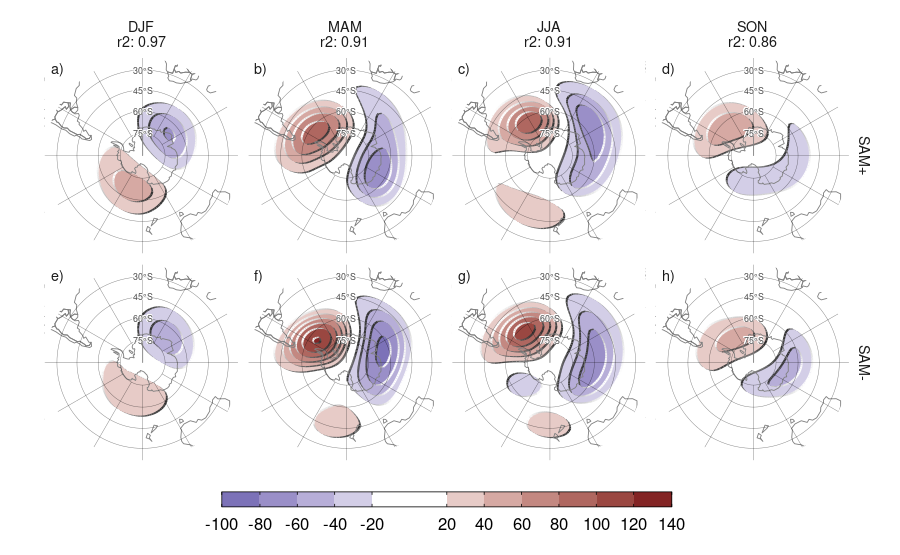
\includegraphics{figures/30-sam/sign-regression-50-1} 

}

\caption{Regresión segmentada de la anomalía zonal de altura geopotencial en 50 hPa con el índice SAM para cada signo para el período 1979--2020 (m). La correlación espacial al cuadrado entre cada campo en cada estación se detalla debajo de la estación. Áreas con puntos marcan regiones donde el p-valor de la diferencia entre el signo positivo y el negativo es menor que 0,01 ajustado por FDR (no hay áreas).}\label{fig:sign-regression-50}
\end{figure}



\begin{figure}

{\centering 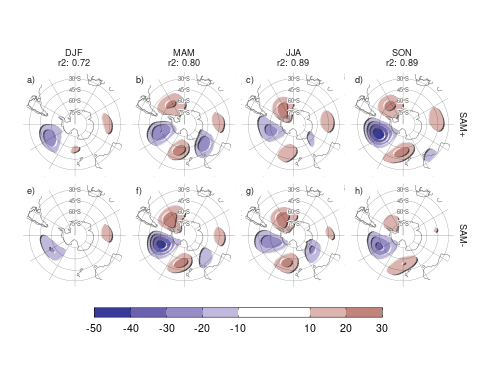
\includegraphics{figures/30-sam/sign-regression-700-1} 

}

\caption{Igual que la Figura \ref{fig:sign-regression-50} pero para 700 hPa.}\label{fig:sign-regression-700}
\end{figure}

Al realizar el análisis EOF utilizando los datos de todos los meses también se asume que la estructura del SAM es la misma en todas las estaciones.
La Figura \ref{fig:season-regression} muestra la regresión de las anomalías de altura geopotencial en 50 y 700 hPa contra el índice SAM para cada trimestre del año y la significancia estadística de la diferencia entre cada estación y SON.

En 50 hPa (Fig. \ref{fig:season-regression} fila a), los patrones del SAM para MAM y JJA son muy similares a SON, con correlación espacial cuadrada mayor a 0,75.
En estas tres estaciones, el SAM en 50 hPa se asocia a una onda planetaria 1 con su centro negativo en 60ºO.
El patrón de JJA tiene algunas diferencias significativas con respecto a SON, principalmente un corrimiento e intensificación de la anomalía negativa de la onda.
El patrón de DEF, en cambio, es muy distinto; la onda 1 tiene su mínimo cerca de 180ºO y está más retraída a latitudes altas.
Además, su correlación espacial es esencialmente nula.

En 700 hPa (Fig. \ref{fig:season-regression} fila b), las cuatro estaciones tienen patrones bastante similares, prácticamente sin diferencias estadísticamente significativas con respecto a SON y con correlaciones cuadradas mayores a 0,6.
El patrón de DEF es el más distinto, siendo similar a SON pero menos intenso.
Esto es consistente con los resultados de Fogt and Marshall (\protect\hyperlink{ref-fogt2020}{2020}).

Estos resultados sugieren entonces que la suposición de estabilidad estacional se cumple excepto para DEF en la estratósfera.
Esto indica que hay que tener cuidado en la interpretación del SAM asimétrico en DEF en la estratosfera ya que el patrón de SAM asimétrico impuesto por la metodología no coincide con el patrón de SAM asimétrico que se obtendría considerando únicamente este trimestre.



\begin{figure}

{\centering 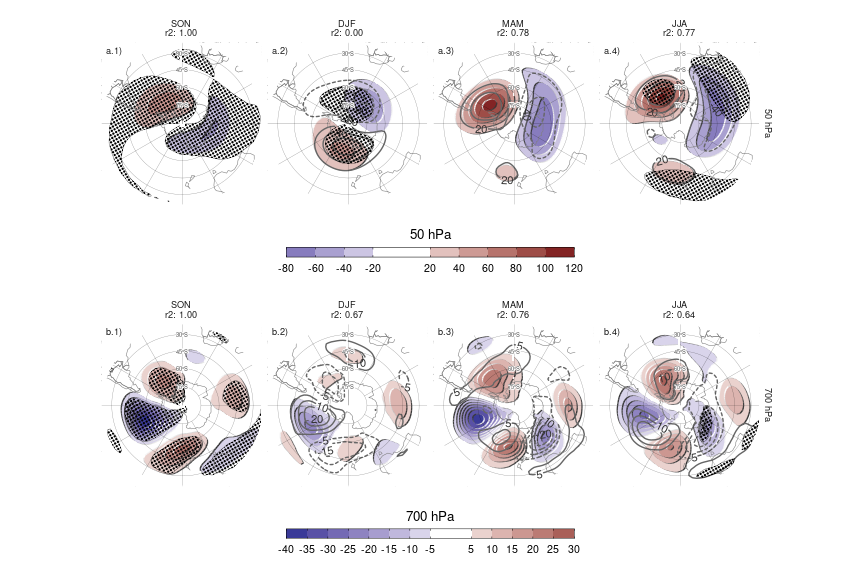
\includegraphics{figures/30-sam/season-regression-1} 

}

\caption{Regresión múltiple de las anomalías zonales de altura geopotencial en 50 hPa y en 700 hPa con el índice SAM para cada estación (m). El sombreado muestra la regresión de cada estación y los contornos grises, la diferencia de cada estación con respecto a SON (valores negativos en línea punteada y positivos en línea sólida). La correlación espacial al cuadrado entre cada campo y el campo de SON se detalla debajo de la estación. Áreas con puntos marcan regiones donde el p-valor es menor que 0,01 ajustado por FDR, donde para estaciones distintas a SON, marca el p-valor de la diferencia respecto a SON.}\label{fig:season-regression}
\end{figure}



\begin{figure}

{\centering 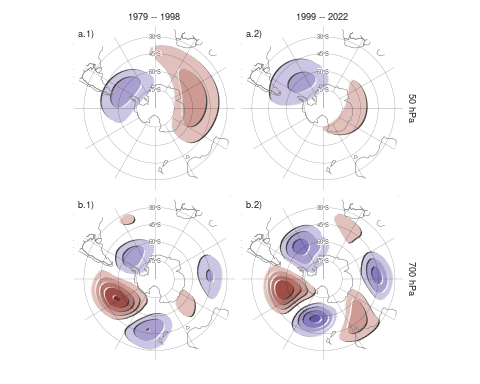
\includegraphics{figures/30-sam/sam-period-1} 

}

\caption{Patrón espacial del primer EOF computado para el período 1979 -- 1998 (columna 1) y 1999 -- 2020 (columna 2) para 50 hPa (fila a) y 700 hPa (fila b). Unidades arbitrarias con valores negativos en azul y negativos en azul.}\label{fig:sam-period}
\end{figure}

El método también asume que el patrón zonalmente asimétrico del SAM permanece estacionario a lo largo del periodo considerado.
Silvestri and Vera (\protect\hyperlink{ref-silvestri2009}{2009}) sugieren que este podría no ser el caso entre 1958 y 2004.
Para probar esta suposición, se calculó el SAM para las dos mitades del periodo (1979 a 1998 y 1999 a 2020), que se muestran en la Figura \ref{fig:sam-period}.
Las diferencias entre los dos períodos parecen ser relativamente pequeñas, tanto en la troposfera como en la estratosfera.
La correlación espacial entre los campos es de 0,73 (CI: 0,72 -- 0,75) en 50 hPa y 0,78 (CI: 0,77 -- 0,79) en 700 hPa.

\hypertarget{resultados-2}{%
\section{Resultados}\label{resultados-2}}

\hypertarget{temporal}{%
\subsection{Evolución temporal}\label{temporal}}

Primero se evalúa la evolución temporal del A-SAM y S-SAM.
La Figura \ref{fig:asymsam-timeseries} muestra las series temporales en 700 hPa y 50 hPa y sus correspondientes estimaciones de densidad.
Se seleccionaron estos dos niveles como representativos de la variabilidad troposférica y estratosférica respectivamente.
Como se muestra a continuación, las variabilidades de ambos índices son muy coherentes dentro de cada región de la atmósfera, por lo que es razonable tomar un nivel como representativo de cada capa.



\begin{figure}

{\centering 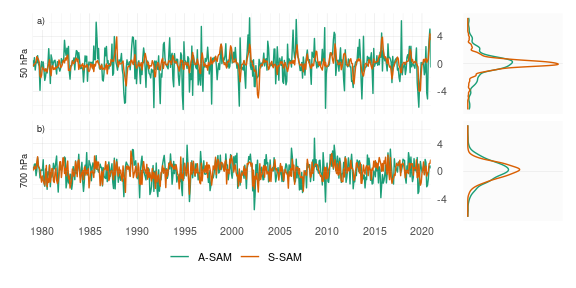
\includegraphics{figures/30-sam/asymsam-timeseries-1} 

}

\caption{Serie temporal de A-SAM y S-SAM en 50 hPa (panel a) y 700 hPa (panel b). A la derecha, la densidad de probabilidad de cada índice. Las series están estandarizadas por el desvío estándar del SAM en cada nivel. Sin unidades.}\label{fig:asymsam-timeseries}
\end{figure}



\begin{figure}

{\centering 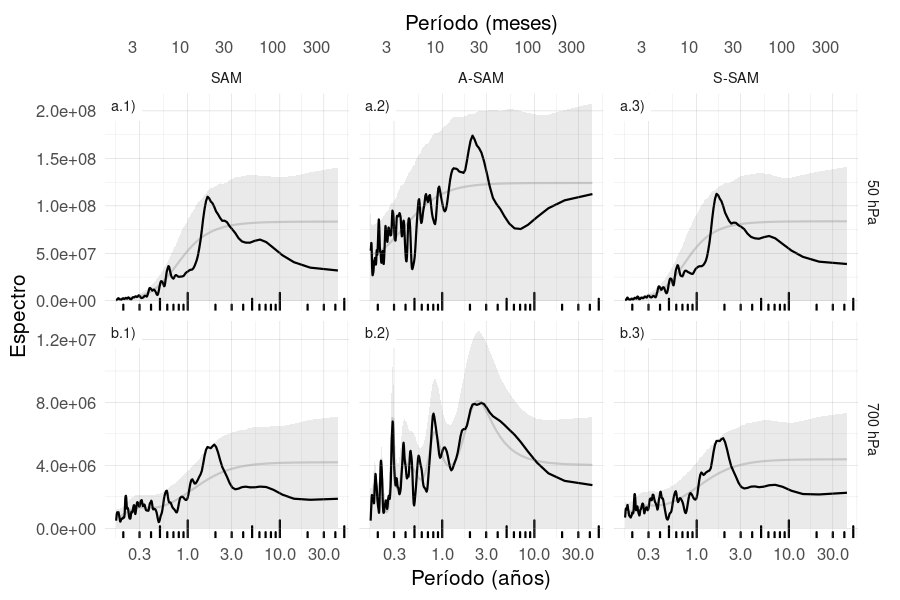
\includegraphics{figures/30-sam/spectrum-1} 

}

\caption{Espectro de cada serie temporal suavizada. El sombreado indica el intervalo de confianza del 95\% del espectro nulo calculado usando bootstrap tomando 5000 simulaciones de un modelo autoregresivo ajustado a los datos. La línea gris indica la amplitud promedio teórica del modelo autoregresivo. Para el período 1979--2020.}\label{fig:spectrum}
\end{figure}

Los espectros de estas series temporales se muestran en la Figura \ref{fig:spectrum}.
El S-SAM estratosférico varía fuertemente con un periodo entre 10 y 30 meses (Fig. \ref{fig:spectrum} a.3).
En el periodograma del S-SAM troposférico (Fig.\ref{fig:spectrum} b.3) se aprecia un pico local en un rango de frecuencias similar, aunque no es estadísticamente significativo.
Esta banda de periodicidad que exhibe la estratosfera está alrededor del rango de periodicidad de la Oscilación Cuasi-Bienal (QBO, por su siglas en inglés, Baldwin et al. (\protect\hyperlink{ref-baldwin2001b}{2001})) y es consistente con los resultados de Vasconcellos et al. (\protect\hyperlink{ref-vasconcellos2022}{2022}), quienes encontraron que el SAM y la QBO comparten una alta potencia común significativa alrededor de la banda de 2 años.
El hecho de que esta periodicidad no sea evidente en el índice A-SAM, también es consistente con los resultados de estos autores, que muestran un monopolo bastante simétrico sobre la Antártida en sus composiciones de anomalías de altura geopotencial durante la QBO oriental y occidental
En la troposfera, el pico de variabilidad más significativo se encuentra en A-SAM en torno a 36 meses.

La Figura \ref{fig:cor-lev} muestra la correlación entre A-SAM y S-SAM en cada nivel para los desfasajes cero (simultáneo) y -1 (A-SAM adelantada a S-SAM en 1 mes).
Los valores de las correlaciones instantáneas entre A-SAM y S-SAM son relativamente constantes en toda la troposfera, fluctuando entre 0,38 y 0,44.
Las correlaciones con defasaje de un mes son igualmente constantes pero muy reducidas.
En la estratosfera, las correlaciones instantáneas caen a un mínimo de 0,28 en 20 hPa y luego aumentan nuevamente monótonamente con la altura hasta el nivel más alto considerado~ (aunque los resultados cerca del tope superior representado en los modelos deben interpretarse con cuidado).
Al mismo tiempo, las correlaciones con un mes de defasaje aumentan con la altura.
Por lo tanto, el índice A-SAM estratosférico tiende a preceder al índice S-SAM.



\begin{figure}

{\centering 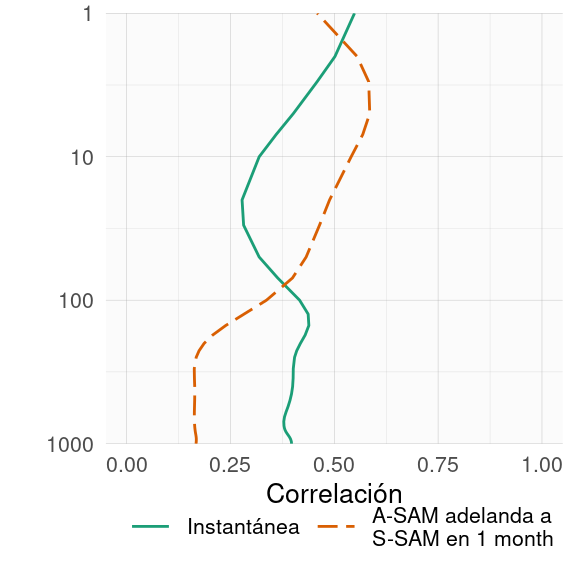
\includegraphics{figures/30-sam/cor-lev-1} 

}

\caption{Correlación instantánea (línea verde) y con un defasaje de 1 mes (línea naranja) entre S-SAM y A-SAM para el período 1979--2020.}\label{fig:cor-lev}
\end{figure}



\begin{figure}

{\centering 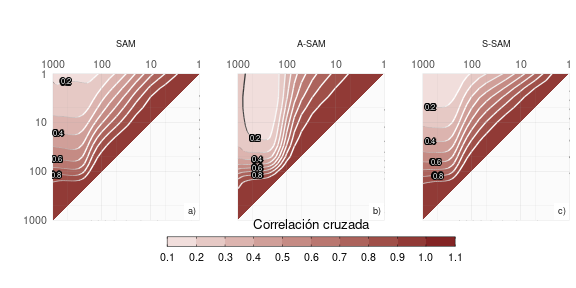
\includegraphics{figures/30-sam/cross-correlation-1} 

}

\caption{Correlación cruzada entre niveles para el índice SAM (a), A-SAM (b) y S-SAM (c) para el período 1979--2020.}\label{fig:cross-correlation}
\end{figure}

La Figura \ref{fig:cross-correlation} muestra la correlación cruzada simultánea (sin desfasaje) entre niveles para los índices SAM, A-SAM y S-SAM.
Para el SAM (Fig. \ref{fig:cross-correlation}a), los valores altos por debajo de 100 hPa reflejan coherencia vertical en toda la troposfera.
Por encima de 100 hPa, la correlación entre niveles disminuye más rápidamente, lo que indica una variabilidad menos coherente.
Sin embargo, las correlaciones entre los niveles troposféricos y los niveles estratosféricos bajos y medios siguen siendo relativamente altas (por ejemplo, más de 0,4 entre los niveles troposféricos y los niveles por debajo de 30 hPa).
A-SAM y S-SAM (Fig. \ref{fig:cross-correlation}b y c, respectivamente) comparten un alto nivel de coherencia similar en la troposfera, pero difieren en su comportamiento estratosférico.
La coherencia estratosférica es mayor para el A-SAM que para el S-SAM.
El S-SAM estratosférico tiene una conexión con el S-SAM troposférico algo más intensa que el A-SAM estratosférico con el A-SAM troposférico.



\begin{figure}

{\centering 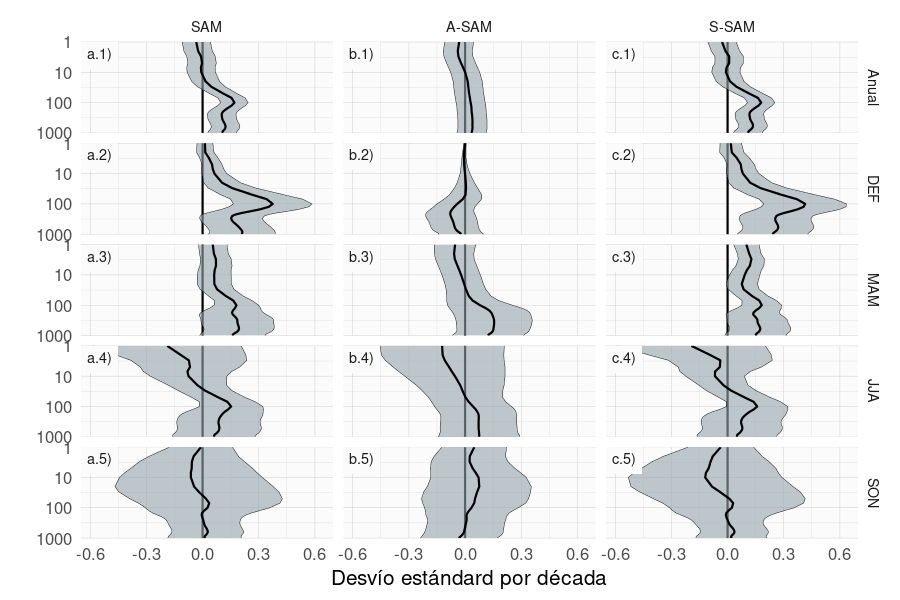
\includegraphics{figures/30-sam/trends-1} 

}

\caption{Tendencias lineales (en desvío estándar por década) del SAM (columna a), A-SAM (columna b) y S-SAM (columna c) para cada nivel usando datos del todo el año (fila 1) y promedios estacionales (filas 2 a 5) para el período 1979--2020. El sombreado indica el intervalo de confianza de 95\%.}\label{fig:trends}
\end{figure}

A continuación, se evalúan las tendencias lineales para cada uno de los índices para el periodo 1979--2020 en cada nivel para el año completo y separado por trimestres (Fig. \ref{fig:trends}).
El índice SAM presenta una tendencia positiva estadísticamente significativa (Fig. \ref{fig:trends}a.1) en todos los niveles entre 1000 hPa y aproximadamente 50 hPa, con un máximo en 100 hPa.
Las tendencias estacionales (Fig. \ref{fig:trends} columna a) indican que las tendencias son significativas sólo en verano y marginalmente en otoño.
Esto es consistente con los resultados de estudios previos, los cuales documentaron tendencias positivas en verano, menores en otoño y ninguna tendencia en las demás estaciones (por ejemplo, Fogt and Marshall (\protect\hyperlink{ref-fogt2020}{2020}) y sus referencias) utilizando índices del SAM basados en la circulación cerca de la superficie.

Al separar el SAM en sus partes asimétrica y simétrica, no sólo se puede ver que estas tendencias se deben casi por completo a la componente simétrica (comparar columnas b y c Figura \ref{fig:trends}), sino que en algunos casos las tendencias se vuelven más claras.
En verano, el índice A-SAM tiene una tendencia negativa estadísticamente no significativa en la troposfera media que oculta la tendencia en el índice SAM; como resultado, las tendencias calculadas utilizando sólo la componente simétrica son más intensas (comparar la región sombreada en la Figura \ref{fig:trends}a.2 y c.2).
En otoño, el índice S-SAM revela una tendencia positiva estadísticamente significativa en la estratosfera que no es significativa utilizando el índice SAM.



\begin{figure}

{\centering 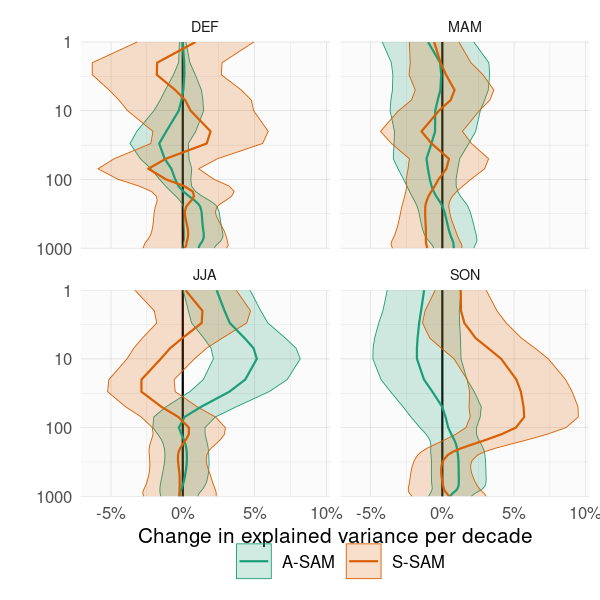
\includegraphics{figures/30-sam/r-squared-trend-1} 

}

\caption{Tendencias lineales (en porcentaje por década) de la varianza explicada por el A-SAM y el S-SAM en cada nivel para cada trimestre en el período 1979--2020. El sombreado indica el intervalo de confianza del 95\%.}\label{fig:r-squared-trend}
\end{figure}

Para estudiar la cuestión de si el SAM se está volviendo más o menos asimétrico, se muestran las tendencias de la varianza explicada de cada índice para cada trimestre en la Figura \ref{fig:r-squared-trend}.
En la troposfera, la única tendencia significativa es la de DEF, en la que el A-SAM tiene una tendencia positiva de alrededor del 2\% por década, lo que sugiere que el SAM en DEF se ha vuelto más asimétrico en el período de 1979 a 2020.
Fogt et al. (\protect\hyperlink{ref-fogt2012}{2012}) observó un cambio de una SAM más asimétrica antes de 1980 a una SAM más simétrica después de 1980, pero nuestro periodo de estudio (1979--2020) nos impide detectar ese cambio.
Sin embargo, debido a la naturaleza atípica de la componente asimétrica del SAM durante la DEF (Sección \ref{definition-of-indices}), esto debe tomarse sólo como una evidencia preliminar.
La otra tendencia significativa se da en la estratosfera durante SON, donde hay una tendencia positiva en la varianza explicada por la S-SAM de aproximadamente un 4\% por década.
Este cambio podría ser el resultado del forzamiento provocado por el agotamiento del ozono.

\hypertarget{spatial}{%
\subsection{Patrones espaciales}\label{spatial}}

Para describir y entender la influencia de las diferentes componentes del SAM en las anomalías temporales de la circulación del hemisferio sur, se calculó la regresión lineal de las anomalías de altura geopotencial sobre los índices SAM, A-SAM y S-SAM en los niveles de 50 hPa y 700 hPa (Fig. \ref{fig:2d-regr}).
Los coeficientes de regresión de la columna 1 de la Figura \ref{fig:2d-regr} se calcularon utilizando el índice del SAM.
Los coeficientes de regresión de las columnas 2 y 3 se calcularon mediante regresión múltiple utilizando los índices A-SAM y S-SAM al mismo tiempo, de manera que deben interpretarse como los patrones asociados a cada índice, eliminando la variabilidad (linealmente) explicada por el otro.



\begin{figure}

{\centering 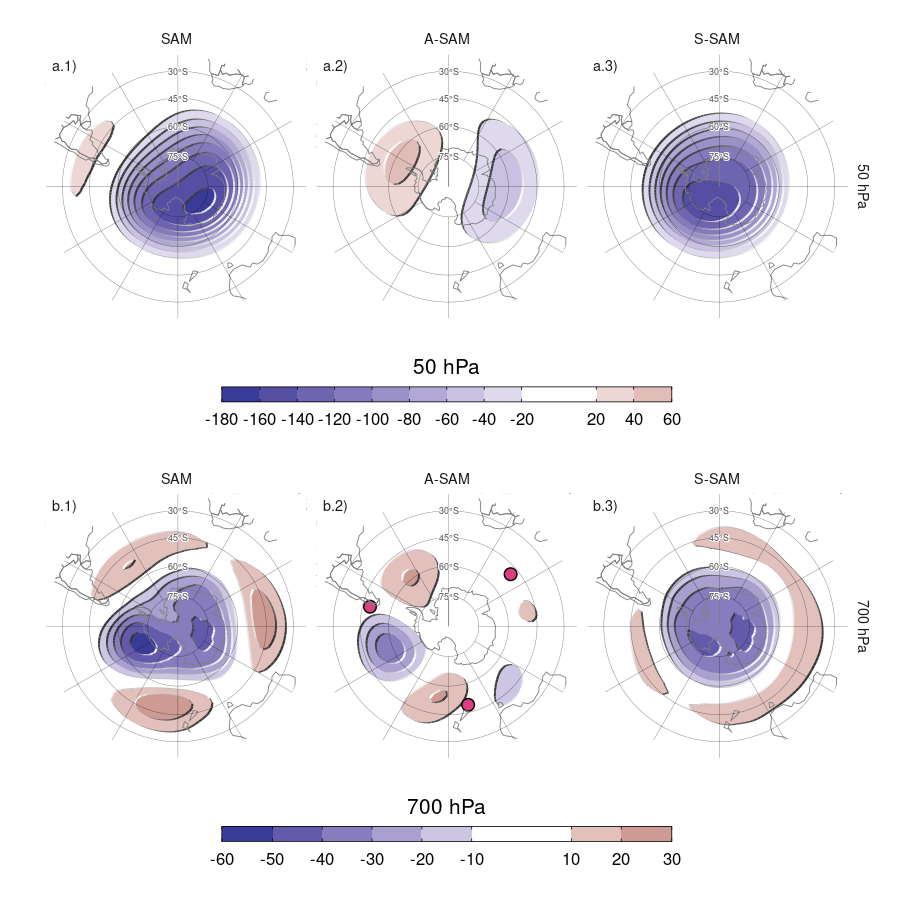
\includegraphics{figures/30-sam/2d-regr-1} 

}

\caption{Regresión de altura geopotencial (metros) en 50 hPa (fila a) y 700 hPa (fila b) con el SAM (columna 1), A-SAM (columna 2) y S-SAM (columna 3) para el período 1979--2020. Los puntos en panel b.2 indican la posición de los puntos de referencia usados por M. N. Raphael (\protect\hyperlink{ref-raphael2004}{2004}) para calcular su índice de la onda zonal 3.}\label{fig:2d-regr}
\end{figure}

En la estratosfera, el patrón espacial descrito por la regresión asociada al SAM está claramente dominado por un monopolo que no está centrado en el Polo Sur (Fig. \ref{fig:2d-regr}a.1).
En cambio, el patrón asociado a la parte asimétrica del SAM se caracteriza por una estructura de onda-1 con centros sobre el Pasaje de Drake en el Hemisferio Occidental y el Mar de Davis en el Hemisferio Oriental.
Este eje se alinea con el defasaje del monopolo encontrado para el SAM (Fig. \ref{fig:2d-regr}.a.1).
Por otra parte, el patrón asociado al S-SAM, es un monopolo más simétrico que el encontrado para el SAM aunque tampoco perfectamente centrado en el Polo Sur.

En la troposfera, el patrón espacial descrito por la regresión asociada al SAM (Fig. \ref{fig:2d-regr}b.1) muestra la ya conocida combinación de una estructura anular zonalmente simétrica en la zona polar con asimetrías zonales en forma de onda-3 en las latitudes medias (\protect\hyperlink{ref-fogt2012}{Fogt et al., 2012}).
Los patrones asociados a los índices A-SAM y S-SAM separan ambas estructuras claramente.
El A-SAM se ve asociado a un patrón de onda zonal 3 y de amplitud modulada por la longitud; con mayor amplitud en hemisferio occidental y casi nula amplitud en el oriental.
El S-SAM, por su parte, se asocia a una estructura anular mucho más zonalmente simétrica que el SAM.
Se encontró que el patrón de onda-3 asociado con el A-SAM (Figura \ref{fig:2d-regr}b.2) está girado media longitud de onda respecto a la posición media del patrón de onda-3 medio descrito por M. N. Raphael (\protect\hyperlink{ref-raphael2004}{2004}), cuyas posiciones de referencia están marcadas con puntos en la figura.
De hecho, no existe correlación entre el índice de M. N. Raphael (\protect\hyperlink{ref-raphael2004}{2004}) y el A-SAM (cor = 0,04 (CI: -0,05 -- 0,13)).
Así, el índice A-SAM troposférico representa un desplazamiento zonal en la posición de la onda 3 climatológica.



\begin{figure}

{\centering 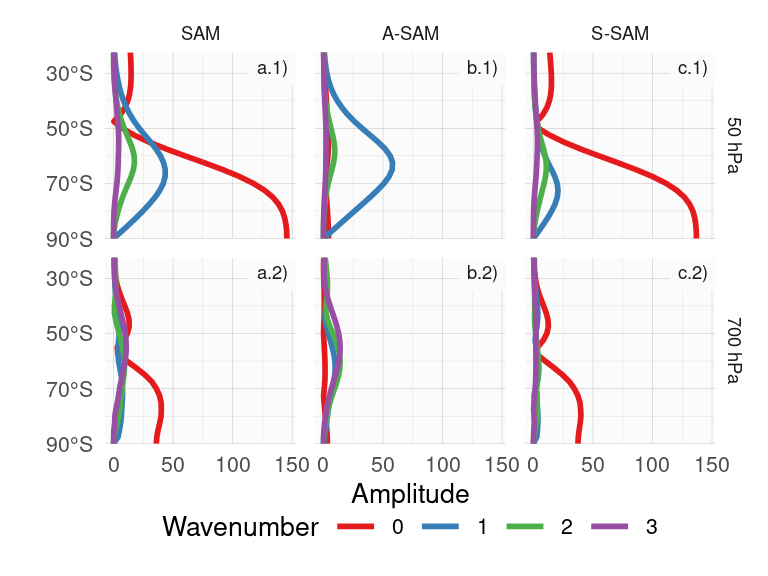
\includegraphics{figures/30-sam/wave-amplitude-1} 

}

\caption{Amplitud (metros) de las ondas zonales de los patrones de regresión de altura geopotencial de la Figura \ref{fig:2d-regr} para ondas zonales con número de onda 0, 1, 2 y 3, donde el número de onda 0 representa la amplitud de la media zonal.}\label{fig:wave-amplitude}
\end{figure}

La amplitud de las ondas zonales con números de onda 0 a 3 en cada latitud a 50 hPa y 700 hPa se muestran en la Figura \ref{fig:wave-amplitude}, donde el número de onda cero representa la amplitud de la media zonal.
Las amplitudes de las ondas zonales del patrón espacial asociado al SAM (Fig. \ref{fig:wave-amplitude} columna a) están dominadas por la media zonal (número de onda 0) en ambos niveles.
Sin embargo, las ondas zonales son importantes, sobre todo al sur de 50ºS, con un número de onda 1 claramente dominante en 50 hPa (Fig. \ref{fig:wave-amplitude}a.1) y una mezcla de ondas de amplitud similar en 700 hPa (Fig. \ref{fig:wave-amplitude}a.2).
La Figura \ref{fig:wave-amplitude} columna b muestra que el A-SAM está dominado principalmente por la onda 1 en la estratosfera (Fig. \ref{fig:wave-amplitude}b.1), mientras que en la troposfera se explica por una combinación de ondas zonales 3 a 1 en nivel decreciente de importancia (Fig. \ref{fig:wave-amplitude}b.2) con una amplitud despreciable de la media zonal.
Por otra parte, el S-SAM se explica casi en su totalidad por la media zonal en ambos niveles (Fig. \ref{fig:wave-amplitude} columna c), con poca o ninguna contribución de las ondas zonales con números de onda de 1 a 3.



\begin{figure}

{\centering 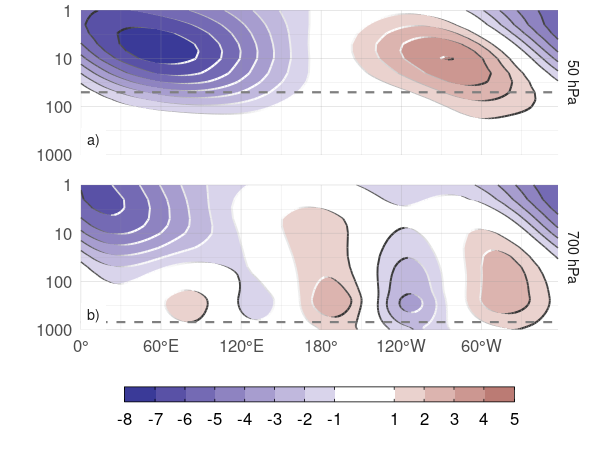
\includegraphics{figures/30-sam/vertical-regression-1} 

}

\caption{Regresión de las anomalías mensuales de altura geopotencial promediada entre 65ºS y 45ºS (metros) y el índice A-SAM de 50 hPa (a) y 700 hPa (b) (niveles indicados en línea punteada) para el período 1979--2020.}\label{fig:vertical-regression}
\end{figure}

La estructura vertical de las anomalías de altura geopotencial asociadas al índice A-SAM se analizaron con mayor profundidad a través de una sección transversal vertical de regresiones de anomalías de altura geopotencial promediadas entre 65ºS y 40ºS con el índice A-SAM de 50 hPa (Fig. \ref{fig:vertical-regression}a) y con el índice A-SAM de 700 hPa (Fig. \ref{fig:vertical-regression}b).
Las anomalías de altura geopotencial asociadas al A-SAM estratosférico (Fig. \ref{fig:vertical-regression}a) están claramente limitadas a la estratosfera, lo que subraya el desacoplamiento entre el A-SAM estratosférico y el troposférico.
La estructura vertical de esta señal se inclina unos 60 grados hacia el oeste entre 100 hPa y 1 hPa, lo que sugiere procesos baroclínicos.
La señal en la estratosfera maximiza cerca de 10 hPa a pesar de utilizar el índice de 50 hPa para la regresión.

El A-SAM troposférico (Fig. \ref{fig:vertical-regression}b) presenta señales significativas que se extienden hacia arriba hasta los niveles más altos del reanálisis.
En la troposfera, la estructura de la onda 3 es barotrópica equivalente, con una amplitud máxima en torno a los 250 hPa.
Las anomalías son mayores en el hemisferio occidental, donde se extienden hasta la estratosfera.
En el hemisferio oriental, la señal de la onda 3 es menor y se limita a la troposfera, mientras que las anomalías negativas dominan en la estratosfera.
Aunque el índice A-SAM troposférico está asociado a anomalías geopotenciales estratosféricas, éstas no se proyectan fuertemente sobre el A-SAM estratosférico.
Las estructuras mostradas en la Figura \ref{fig:vertical-regression} son robustas a la elección del nivel del índice.
Para cualquier índice estratosférico (por encima de 100 hPa), las anomalías resultantes son muy similares a la estructura de onda-1 con máximo cerca de 10 hPa en la Figura \ref{fig:vertical-regression}a.
Por el contrario, para cualquier índice troposférico (por debajo de 100 hPa), el resultado es muy similar al de la Figura \ref{fig:vertical-regression}b.
Los patrones cambian principalmente en amplitud (no se muestra).



\begin{table}

\caption{\label{tab:enso-cor-table}Correlación entre los índices del SAM y el ONI considerando todos los meses y para cada estación por separado. Entre parentéresis se indican los p-valores ajustado por FDR). En negrita, se indican las correlaciones con p-valores menores a 0,01.}
\centering
\begin{tabular}[t]{c>{}c>{}c>{}c}
\toprule
\multicolumn{1}{c}{ } & \multicolumn{1}{c}{Correlación} & \multicolumn{2}{c}{Correlación parcial} \\
\cmidrule(l{3pt}r{3pt}){2-2} \cmidrule(l{3pt}r{3pt}){3-4}
 & SAM & A-SAM & S-SAM\\
\midrule
 & \textbf{-0,17} & \textbf{-0,25} & 0,00\\
\cmidrule{2-4}
\multirow[t]{-2}{*}{\centering\arraybackslash Año} & \textbf{(<0,001)} & \textbf{(<0,001)} & (0,993)\\
\cmidrule{1-4}
 & \textbf{-0,32} & \textbf{-0,31} & -0,19\\
\cmidrule{2-4}
\multirow[t]{-2}{*}{\centering\arraybackslash DEF} & \textbf{(<0,001)} & \textbf{(0,002)} & (0,068)\\
\cmidrule{1-4}
 & -0,05 & \textbf{-0,25} & 0,15\\
\cmidrule{2-4}
\multirow[t]{-2}{*}{\centering\arraybackslash MAM} & (0,678) & \textbf{(0,009)} & (0,156)\\
\cmidrule{1-4}
 & 0,02 & -0,13 & 0,11\\
\cmidrule{2-4}
\multirow[t]{-2}{*}{\centering\arraybackslash JJA} & (0,948) & (0,218) & (0,300)\\
\cmidrule{1-4}
 & \textbf{-0,26} & \textbf{-0,40} & 0,00\\
\cmidrule{2-4}
\multirow[t]{-2}{*}{\centering\arraybackslash SON} & \textbf{(0,008)} & \textbf{(<0,001)} & (0,993)\\
\bottomrule
\end{tabular}
\end{table}

El patrón de la onda 3 de la Figura \ref{fig:2d-regr}b.2 es muy similar al PSA (\protect\hyperlink{ref-kidson1988}{Kidson, 1988}; \protect\hyperlink{ref-mo1987}{Mo and Ghil, 1987}), que es un patrón de teleconexión asociado al ENSO (\protect\hyperlink{ref-karoly1989}{Karoly, 1989}).
Como se mencionó en la introducción de este capítulo, existen evidencias previas de que la actividad del ENSO y el SAM pueden estar relacionadas (\protect\hyperlink{ref-fogt2011a}{Fogt et al., 2011}; \protect\hyperlink{ref-silvestri2009}{Silvestri and Vera, 2009}).
Se analizó entonces la relación entre el SAM y sus componentes y el ENSO (medido por el Índice del Niño Oceánico (ONI, \protect\hyperlink{ref-bamston1997}{Bamston et al., 1997})) y se muestra en la Tabla \ref{tab:enso-cor-table} para cada índice SAM y para cada trimestre y para todo el año.
Mientras que la correlación es significativa entre el SAM completo y ENSO considerando todo el año, solamente es significativa para los trimestres DEF y SON.
Se encontró que esta relación es captada principalmente por el A-SAM, ya que este índice presenta correlaciones parciales significativas con el ENSO, mientras que las correlaciones con el S-SAM son todas menores y no significativas.
Incluso en los trimestres donde la correlación entre SAM y ENSO es esencialmente nula (MAM y JJA), la correlación parcial entre el A-SAM y el ONI es mucho más alta; en efecto, en MAM es significativa al nivel del 95\%.
El mismo análisis se realizó utilizando el Índice ENSO Multivariado (\protect\hyperlink{ref-wolter2011}{Wolter and Timlin, 2011}) y el Índice de Oscilación del Sur (\protect\hyperlink{ref-ropelewski1987}{Ropelewski and Jones, 1987}), obteniendo resultados similares.
Esto último indica que estos resultados no dependen del índice ENSO utilizado.

\hypertarget{impacts}{%
\subsection{Impactos}\label{impacts}}

Para evaluar las diferencias en los impactos asociados a los índices SAM, A-SAM y S-SAM, se realió una regresión de la temperatura del aire a 2 metros y la precipitación sobre cada uno de los tres índices del SAM de 700 hPa.
Como se mostró en secciones anteriores, los tres índices son muy coherentes en la troposfera, por lo que se seleccionó este nivel para representar la circulación troposférica por compatibilidad con la literatura previa.
Las regresiones se realizaron sin quitarle la tendencia ni a las variables ni a los índices, pero el cálculo de las regresiones con valores sin tendencias no muestran diferencias importantes (no se muestra).

\hypertarget{temperatura-del-aire-a-2-metros}{%
\subsubsection{Temperatura del aire a 2 metros}\label{temperatura-del-aire-a-2-metros}}

La Figura \ref{fig:regr-air-season} muestra las regresiones con la temperatura del aire a 2 metros.
En verano, los valores positivos del índice SAM (Fig. \ref{fig:regr-air-season}a.1) se asocian con anomalías negativas de temperatura cerca de la Antártida rodeadas por un anillo de anomalías positivas en las latitudes medias.
El anillo no es zonalmente simétrico, ya que hay cuatro máximos locales distintivos en torno a 30ºO, 120ºO, 150ºE y 90ºE respectivamente.
En los trópicos, las anomalías son negativas en el Pacífico ecuatorial, lo que concuerda con la correlación negativa entre SAM y ENSO observada en la Tabla \ref{tab:enso-cor-table}.
Los paneles a.2 y a.3 de la Figura \ref{fig:regr-air-season} muestran que tanto las anomalías negativas en los trópicos como las anomalías entre 45ºS y 60ºS están asociadas principalmente con el A-SAM y que el S-SAM está asociado a anomalías de temperatura extendidas más zonalmente simétricas en latitudes altas.
Sobre la Antártida, los valores positivos del índice SAM están asociados a anomalías negativas de temperatura, en particular sobre la costa oriental.
Estas anomalías están explicadas únicamente con el S-SAM.
Por otro lado, las anomalías de temperatura en el océano Índico, el sur de África y Australia están fuertemente relacionadas con A-SAM y no están presentes en el patrón asociado con el SAM.



\begin{figure}

{\centering 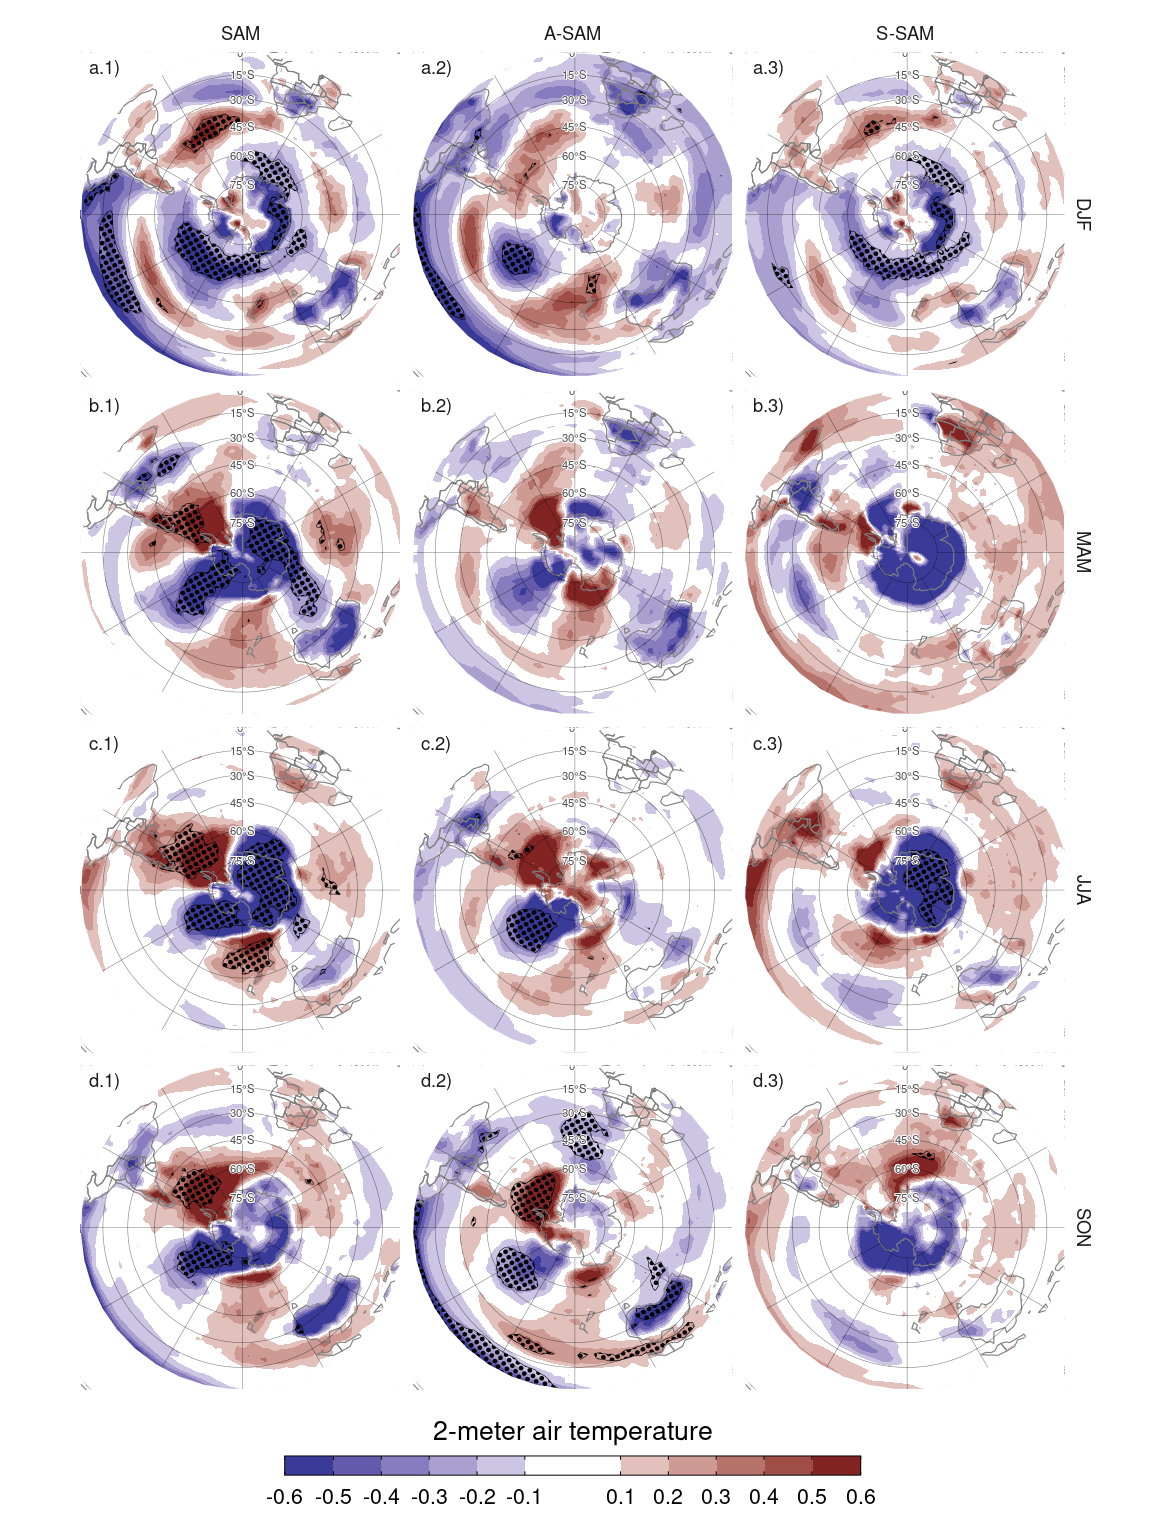
\includegraphics{figures/30-sam/regr-air-season-1} 

}

\caption{Regresión de las anomalías de temperatura a dos metros (K) con el índice SAM (columna a), A-SAM (columna b) y S-SAM (columna c) en cada trimestre para el período 1979--2020. Áreas con puntos marcan regiones donde el p-valor es menor que 0,01 ajustado por FDR. La escala de colores se corta en \(\pm0,6 \mathrm{K}\) para resaltar valores de regresión en los trópicos y latitudes medias a expensas de los valores en las regiones polares.}\label{fig:regr-air-season}
\end{figure}

En otoño, invierno y primavera (filas b, c y d en la Figura \ref{fig:regr-air-season}) el SAM está asociado a anomalías de temperatura con estructura zonalmente asimétrica en latitudes altas, con valores negativos sobre la Antártida y el Mar de Amundsen y positivas al sur de Nueva Zelanda y centradas en el pasaje de Drake que se extienden hasta la Patagonia.
Esto refleja la naturaleza más asimétrica del SAM durante estas estaciones en comparación al verano.
En acuerdo, M. E. Jones et al. (\protect\hyperlink{ref-jones2019}{2019}) observó características similares en las mediciones de estaciones, aunque utilizando datos de 1957 a 2016.
De todas maneras, en general se observa que la señal sobre la Antártida está asociada al S-SAM (aunque estadísticamente significativa sólo en invierno), mientras que las anomalías sobre el Océano Antártico y latitudes más bajas se asocian al A-SAM.
En primavera, la señal tropical de A-SAM es similar a la del verano, revelando de nuevo la importancia del vínculo ENSO-\/-A-SAM.

El patrón de anomalías de temperatura negativas en el polo rodeadas de anomalías positivas, evidente aproximadamente en todas las estaciones -aunque con intensidad variable y detalles a pequeña escala-, se traduce en un gradiente de temperatura meridional aumentado que maximiza en la línea cero, lo que es coherente con la intensificación y migración hacia el polo de los vientos del oeste comúnmente vinculados al SAM a través del balance de viento térmico.
Por tanto, no es sorprendente verlo más claramente asociado al S-SAM.
Asimismo, las temperaturas sobre la Antártida Oriental se ven más afectadas por el S-SAM, mientras que en la Antártida Occidental son más sensibles al A-SAM.
Dado que el índice S-SAM está negativamente correlacionado con la temperatura sobre la Antártida Oriental (Figura \ref{fig:regr-air-season} columna 3), es posible que la tendencia positiva en el índice S-SAM pueda ayudar a explicar la falta de tendencia positiva de la temperatura en la Antártida Oriental en comparación con la Antártida Occidental en el contexto del calentamiento global (\protect\hyperlink{ref-nicolas2014}{Nicolas and Bromwich, 2014}).

\hypertarget{precipitaciuxf3n}{%
\subsubsection{Precipitación}\label{precipitaciuxf3n}}

La Figura \ref{fig:global-pp} muestra la regresión de los índices SAM con la precipitación para el hemisferio sur considerando todos los meses del año.
La señal de precipitación asociada al SAM completo (Fig. \ref{fig:global-pp}a) muestra en general una disminución de la precipitación en torno a los 45ºS, un ligero aumento de la precipitación en torno a los 30ºS y un aumento de la precipitación sobre la Antártida, un patrón que concuerda con los obtenidos en otros estudios (p.ej. \protect\hyperlink{ref-hendon2014}{Hendon et al., 2014}).
Este patrón se mantiene prácticamente sin cambios entre estaciones, aunque varía en intensidad (no se muestra).
Los paneles b y c de la Figura \ref{fig:global-pp} muestran que la influencia del A-SAM sólo se da en los trópicos y latitudes medias, mientras que la señal S-SAM es fuerte en las latitudes altas.
En particular, los valores positivos del S-SAM se asocian con el aumento de las precipitaciones sobre la Antártida y la disminución de las precipitaciones alrededor del Océano Austral.



\begin{figure}

{\centering 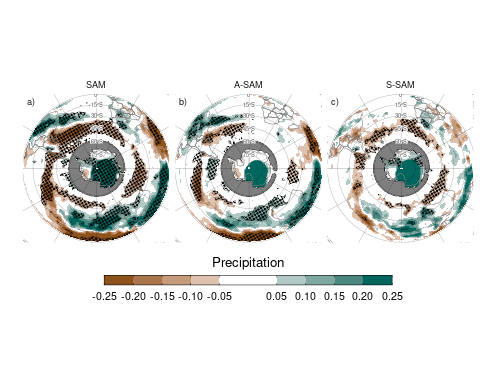
\includegraphics{figures/30-sam/global-pp-1} 

}

\caption{Regresión de anomalías de precipitación (mm por día) con el SAM (a), A-SAM (b) y S-SAM (c) para el período 1979--2020. En gris, las zonas con valores faltantes. Áreas con puntos marcan regiones donde el p-valor es menor que 0,01 ajustado por FDR. La escala de colores se corta en \(\pm0,25 \mathrm{K}\) para resaltar valores de regresión en los trópicos y latitudes medias a expensas de los valores en las regiones polares.}\label{fig:global-pp}
\end{figure}

Para estudiar con más detalle los impactos locales en distintas regiones continentales del hemisferio sur, las Figuras \ref{fig:pp-regr-oceania} y \ref{fig:pp-regr-america} muestran la regresión de los índices SAM con la precipitación media estacional y la altura geopotencial de 700 hPa para la región de Oceanía, y Sudamérica respectivamente.
No se muestran los resultados para la región de Sudáfrica porque allí no se detectó ninguna señal significativa.



\begin{figure}

{\centering 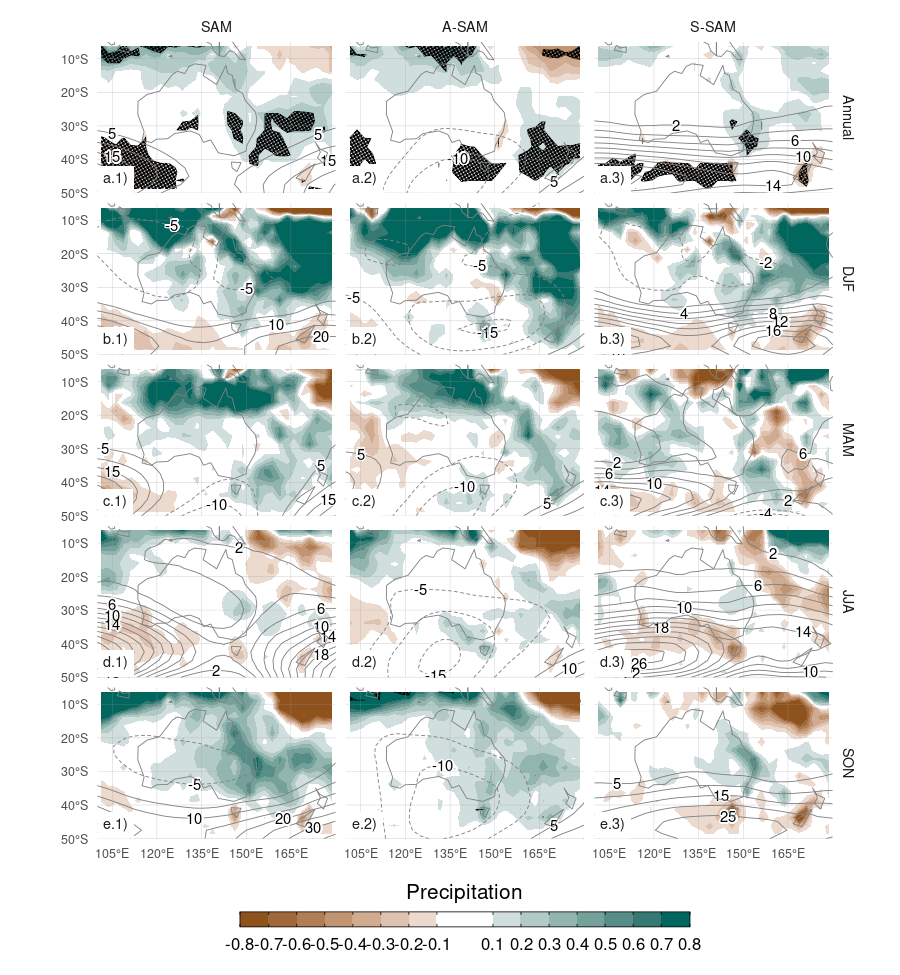
\includegraphics{figures/30-sam/pp-regr-oceania-1} 

}

\caption{Regresión de anomalías de precipitación (mm por día, sombrado) y anomalías de altura geopotencial (líneas finas, valores positivos en líneas llenas y negativos en líneas punteadas) para todo el año (fila a) y medias estacionales (filas b a e) con el SAM (columna 1), A-SAM (columna 2) y S-SAM (columna 3) para el período 1979--2020. Nueva Zelanda e islas aledañas. Áreas con puntos marcan regiones donde el p-valor es menor que 0,01 ajustado por FDR.}\label{fig:pp-regr-oceania}
\end{figure}

En Oceanía, la regresión anual muestra que el índice SAM está asociado con anomalías positivas de precipitación en la región sudeste de Australia (Fig. \ref{fig:pp-regr-oceania}a.1), en acuerdo con Gillett et al. (\protect\hyperlink{ref-gillett2006}{2006}).
La separación entre A-SAM y S-SAM sugiere que esta anomalía positiva se explica por el S-SAM sólo en la costa este (Fig. \ref{fig:pp-regr-oceania}c.1).
Las anomalías de altura geopotencial asociadas a este índice (contornos negros) son indicativas de un flujo hacia el oeste procedente del mar de Tasmania, lo que podría explicar las anomalías positivas en las precipitaciones, en acuerdo con Hendon et al. (\protect\hyperlink{ref-hendon2007}{2007}).
El A-SAM parece estar relacionado con anomalías positivas de precipitación en la costa sureste de Australia (Fig. \ref{fig:pp-regr-oceania}b.2), que podrían explicarse de forma similar por la circulación anómala del oeste que transporta aire húmedo al continente desde el océano Índico.

Las regresiones estacionales muestran valores altos pero no estadísticamente significativos.
En SON, valores positivos del SAM se asocian con anomalías positivas de precipitación en el este y centro de Australia (Fig. \ref{fig:pp-regr-oceania}a.5).
En este trimestre, el S-SAM parece estar asociado con anomalías positivas de precipitación en un área relativamente reducida de la costa oriental (Fig. \ref{fig:pp-regr-oceania}c.5) mientras que las anomalías positivas de precipitación relacionadas con A-SAM positivo afectan a todo el este de Australia (Fig. \ref{fig:pp-regr-oceania}b.5).

En verano, un índice SAM positivo se asocia con anomalías de precipitación positivas en Australia occidental y oriental, sobre todo en la región noreste (Fig. \ref{fig:pp-regr-oceania}a.2).
La parte oriental está dominada por la relación con el S-SAM y la occidental, por el A-SAM.
En otoño, la regresión con el SAM muestra anomalías positivas en el norte, similares a las de verano, que se asocian con el A-SAM.
En invierno los coeficientes de regresión son mucho más débiles que durante el resto del año.
Ninguno de estos coeficientes de regresión es estadísticamente significativo al nivel del 95\%.
La señal de la primavera coincide en líneas generales con Hendon et al. (\protect\hyperlink{ref-hendon2007}{2007}), pero mientras que ellos también detectaron una fuerte señal en verano, la Figura \ref{fig:pp-regr-oceania}a.2 no muestra ninguna asociación estadísticamente significativa (aunque los coeficientes tienen un signo coherente).



\begin{figure}

{\centering 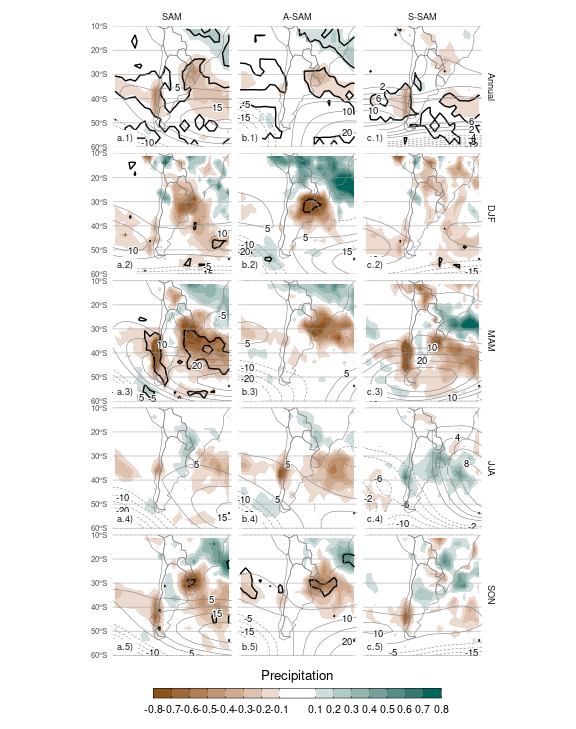
\includegraphics{figures/30-sam/pp-regr-america-1} 

}

\caption{Igual que la Figura \ref{fig:pp-regr-oceania} pero para Sudamérica.}\label{fig:pp-regr-america}
\end{figure}

En Sudamérica (Fig. \ref{fig:pp-regr-america}), la regresión anual muestra que la fase positiva del SAM está asociada con anomalías de precipitación negativas en el SESA y el sur de Chile, y anomalías positivas en el sudeste de Brasil, alrededor de la posición climatológica de la Zona de Convergencia del Atlántico Sur (SACZ) (Fig. \ref{fig:pp-regr-america}a.1).
Las figuras \ref{fig:pp-regr-america}a.2 y a.3 muestran que mientras las señales sobre SESA y el sudeste de Brasil están asociadas significativamente con A-SAM, la del sur de Chile está relacionada con S-SAM.

Las regresiones estacionales reflejan un patrón similar al annual, excepto en invierno.
Aunque no sean estadísticamente significativas, todas las estaciones muestran valores negativos en SESA y el sur de Chile junto con valores positivos en el sur de Brasil en relación con el SAM.
La separación de estas características entre los mapas de regresión del A-SAM y S-SAM es también bastante consistente.
En invierno la señal del SAM es levemente positiva en el SESA y al sur de Chile y levemente negativa en el centro de Chile.

La circulación anómala a 700 hPa asociada al S-SAM (Fig. \ref{fig:pp-regr-america}a.3) indica un flujo anómalo del este sobre el sur de Chile.
Esto conduce a una menor advección de aire húmedo desde el Océano Pacífico, que es la principal fuente de agua precipitable en esa región (\protect\hyperlink{ref-garreaud2007}{Garreaud, 2007}).
Por otro lado, la circulación anómala asociada a valores positivos del A-SAM (Fig. \ref{fig:pp-regr-america}a.2) en el Atlántico es anticiclónica al este y ciclónica al oeste de Sudamérica.
Esto promueve un flujo anómalo del sudeste sobre el SESA que inhibe el flujo del chorro de baja altura desde Sudamérica hacia la región (p.ej. \protect\hyperlink{ref-silvestri2009}{Silvestri and Vera, 2009}; \protect\hyperlink{ref-zamboni2010}{Zamboni et al., 2010}).
Se encontró que este mismo patrón está asociado con el aumento de las precipitaciones en el sur de Brasil durante los eventos de SACZ (\protect\hyperlink{ref-rosso2018}{Rosso et al., 2018}).

\hypertarget{sam-ceof}{%
\subsection{Relación con los cEOFs}\label{sam-ceof}}

Se evaluó también la relación de los cEOFs presentados en el Capítulo \ref{ceofs} con los índices del SAM.
Para ello, se calculó el coeficiente de determinación entre las series temporales de los cEOFs con cada uno de los índices SAM definidos en cada nivel vertical (Fig.~\ref{fig:sam-eof-vertical}).
Dado que los cEOFs fueron definidos únicamente para el trimestre SON, esto se calculó sólo para estre trimestre.
El índice SAM está correlacionado de forma estadísticamente significativa con la fase de 0º del cEOF1 en todos los niveles, y con la fase de 90º del cEOF1 y la fase de 90º del cEOF2 en la tropósfera.
Por otro lado, las correlaciones entre el SAM y la fase de 0º del cEOF2 son prácticamente nulas.



\begin{figure}

{\centering 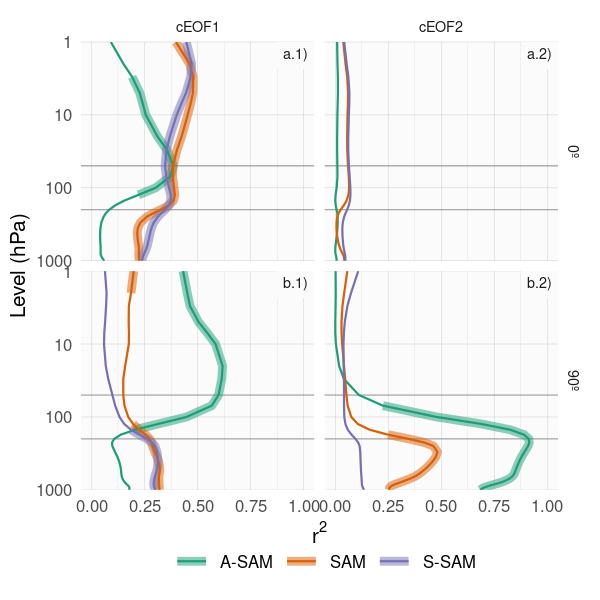
\includegraphics{figures/30-sam/sam-eof-vertical-1} 

}

\caption{Coeficiente de determinación (\(r^2\)) entre la fase de 0º (fila a) y 90º (fila b) de los cEOFs con el SAM (línea naranja), A-SAM (línea verde) y S-SAM (línea azul) para cada nivel durante el período 1979--2020 para SON. Las líneas gruesas representan valores con p-valor menor a 0,01 ajustado por FDR.}\label{fig:sam-eof-vertical}
\end{figure}

En la tropósfera la correlación de ambas fases del cEOF1 y el SAM es igual a su correlación con el S-SAM, y su correlación con el A-SAM es mucho más baja y no significativa.
Esto indica que la relación entre el SAM y el cEOF1 en la tropósfera se explica en su totalidad por la componente zonalmente simétrica del SAM.
En la estratosfera, la fase de 0º del cEOF1 está correlacionada tanto con el A-SAM como con la S-SAM, mientras que la fase de 90º está altamente correlacionada sólo con el A-SAM.
Estas correlaciones son consistentes con los mapas de regresión de la altura geopotencial en la Figura \ref{fig:eof1-regr-gh} y su comparación con los obtenidos para SAM, A-SAM y S-SAM (Fig. \ref{fig:2d-regr}).

La Figura \ref{fig:sam-eof-vertical} muestra que el cEOF2 sólo tiene relación con el SAM en su fase de 90º, asociada a la parte asimétrica y únicamente en la tropósfera.
La correlación entre ambos índices es muy alta, con valores superiores al 75\% de la varianza compartida en toda la tropósfera y un máximo de 92\% en 225 hPa.
Esta altísima correlación es comparable a la correlación observada entre distintos índices del SAM (Ho et al. (\protect\hyperlink{ref-ho2012}{2012})).
Esto sugiere que la fase de 90º del cEOF2 es capaz de caracterizar la actividad de la componente zonalmente asimétrica de el SAM en su totalidad.

\hypertarget{conclusiones-del-capuxedtulo-refasymsam}{%
\section{Conclusiones del capítulo \ref{asymsam}}\label{conclusiones-del-capuxedtulo-refasymsam}}

La división del SAM entre su parte zonalmente asimétrica y simétrica muestra que estos dos aspectos del SAM tienen variabilidad, tendencias e impactos distintivos que merecen ser abordados por separado.

Los patrones asociados al S-SAM son mucho más anulares que los asociados al SAM en toda la atmósfera.
En la tropósfera, el A-SAM describe un patrón de onda zonal 3 similar al cEOF2 que se extiende verticalmente en toda esta capa y alcanza su máximo en 250 hPa y explica la relación entre el SAM y el ENSO.
En la estratósfera describe un patrón de onda 1 similar al cEOF1.

La relación entre el SAM y el cEOF1 en la tropósfera se explica en su totalidad por la componente zonalmente simétrica del SAM, mientras que la relación entre el cEOF2 y el SAM se explica por la relación entre la fase de 90º del cEOF2 y la parte asimétrica del SAM.

Esto último sugiere que el A-SAM no es una componente intrínseca del SAM, sino que es la respuesta de la circulación atmosférica a la influencia tropical que aparece reflejado en el primer EOF de las anomalías de altura geopotencial por construcción.

Los principales resultados de este capítulo han sido publicados en Campitelli et al. (\protect\hyperlink{ref-campitelli2022}{2022}).

\hypertarget{cmip6}{%
\chapter{Análisis de los modos de variabilidad de la circulación zonalmente asimétrica en los modelos del CMIP6}\label{cmip6}}

El análisis previo estudió la circulación zonalmente asimétrica en los datos de reanálisis.
Sin embargo, el estudio de tendencias y variabilidad de estos modelos se ve limitada por la corta longitud de los datos observacionales y la posible inhomogeneidad del reanálisis al cambiar la densidad y tipo de observaciones; un problema que afecta particularmente al hemisferio sur.
Además, es imposible abordar la atribución de las tendencias observadas a sus posibles causas utilizando únicamente observaciones.

Estas limitaciones motivan completar el trabajo de tesis a partir de la utilización de salidas de modelos climáticos.
En este capítulo se analiza la habilidad de los modelos del sexto Proyecto de Intercomparación de Modelos Acoplados (CMIP6) (\protect\hyperlink{ref-eyring2016}{Eyring et al., 2016}) y del Proyecto de Intercomparación de Modelos de Detección y Atribución (DAMIP) (\protect\hyperlink{ref-gillett2016}{Gillett et al., 2016}) de capturar estos modos y sus principales características.
Al contar con corridas mucho más largas y múltiples miembros por modelo, es posible evaluar las tendencias a largo plazo con mayor robustez.
Utilizando los modelos incluidos en DAMIP, además es posible avanzar en la atribución de las tendencias observadas.
Por lo que también se utilizaron las simulaciones de DAMIP para explicar los forzantes asociados con las tendencias observadas en los modos de variabilidad de la circulación zonalmente asimétrica del hemisferio sur.

Estudios previos evaluaron las tendencias de los principales modos de circulación del hemisferio sur.
Encontraron que la tendencia positiva del SAM observada en el clima presente es simulada correctamente por los modelos de CMIP5 y CMIP6 y que puede atribuirse tanto al efecto del incremento de los gases de efecto invernadero como a la destrucción del ozono estratosférico (\protect\hyperlink{ref-gillett2013}{Gillett et al., 2013}; \protect\hyperlink{ref-ipcc6ch3}{Intergovernmental Panel on Climate Change (IPCC), 2023}).

\hypertarget{muxe9todos-2}{%
\section{Métodos}\label{muxe9todos-2}}

\hypertarget{datos-3}{%
\subsection{Datos}\label{datos-3}}

El CMIP6 es un proyecto que convoca y coordina a numerosos centros de modelado climático para realizar experimentos numéricos relacionados con el Cambio Climático, bajo protocolos comunes.
Los conjuntos de datos de los diferentes CMIP han sido un insumo fundamental en la elaboración de los reportes del IPCC.
DAMIP es una componente del CMIP6 que cuenta con experimentos particularmente diseñados para realizar estudios de atribución.

\begin{longtable}[]{@{}
  >{\raggedright\arraybackslash}p{(\columnwidth - 10\tabcolsep) * \real{0.6277}}
  >{\raggedleft\arraybackslash}p{(\columnwidth - 10\tabcolsep) * \real{0.0803}}
  >{\raggedleft\arraybackslash}p{(\columnwidth - 10\tabcolsep) * \real{0.0657}}
  >{\raggedleft\arraybackslash}p{(\columnwidth - 10\tabcolsep) * \real{0.0657}}
  >{\raggedleft\arraybackslash}p{(\columnwidth - 10\tabcolsep) * \real{0.0657}}
  >{\raggedleft\arraybackslash}p{(\columnwidth - 10\tabcolsep) * \real{0.0949}}@{}}
\caption{\label{tab:modelos}Modelos analizados y la cantidad de miembros para cada experimento.}\tabularnewline
\toprule()
\begin{minipage}[b]{\linewidth}\raggedright
Modelo
\end{minipage} & \begin{minipage}[b]{\linewidth}\raggedleft
historical
\end{minipage} & \begin{minipage}[b]{\linewidth}\raggedleft
hist-GHG
\end{minipage} & \begin{minipage}[b]{\linewidth}\raggedleft
hist-nat
\end{minipage} & \begin{minipage}[b]{\linewidth}\raggedleft
hist-aer
\end{minipage} & \begin{minipage}[b]{\linewidth}\raggedleft
hist-stratO3
\end{minipage} \\
\midrule()
\endfirsthead
\toprule()
\begin{minipage}[b]{\linewidth}\raggedright
Modelo
\end{minipage} & \begin{minipage}[b]{\linewidth}\raggedleft
historical
\end{minipage} & \begin{minipage}[b]{\linewidth}\raggedleft
hist-GHG
\end{minipage} & \begin{minipage}[b]{\linewidth}\raggedleft
hist-nat
\end{minipage} & \begin{minipage}[b]{\linewidth}\raggedleft
hist-aer
\end{minipage} & \begin{minipage}[b]{\linewidth}\raggedleft
hist-stratO3
\end{minipage} \\
\midrule()
\endhead
AWI-CM-1-1-MR & & & & & \\
(\protect\hyperlink{ref-CMIP6.CMIP.AWI.AWI-CM-1-1-MR}{Semmler et al., 2018}) & 10 & - & - & - & - \\
FGOALS-g3 & & & & & \\
(\protect\hyperlink{ref-CMIP6.CMIP.CAS.FGOALS-g3}{Li, 2019}, \protect\hyperlink{ref-CMIP6.DAMIP.CAS.FGOALS-g3}{2020}) & 12 & 3 & 3 & - & - \\
CanESM5 & & & & & \\
(\protect\hyperlink{ref-CMIP6.CMIP.CCCma.CanESM5}{Swart et al., 2019a}, \protect\hyperlink{ref-CMIP6.DAMIP.CCCma.CanESM5}{2019b}) & 50 & 50 & 50 & 10 & 10 \\
CNRM-CM6-1 & & & & & \\
(\protect\hyperlink{ref-CMIP6.CMIP.CNRM-CERFACS.CNRM-CM6-1}{Voldoire, 2018}, \protect\hyperlink{ref-CMIP6.DAMIP.CNRM-CERFACS.CNRM-CM6-1}{2019}) & 60 & 10 & 10 & 10 & - \\
CNRM-ESM2-1 & & & & & \\
(\protect\hyperlink{ref-CMIP6.CMIP.CNRM-CERFACS.CNRM-ESM2-1}{Seferian, 2018}) & 21 & - & - & - & - \\
ACCESS-ESM1-5 & & & & & \\
(\protect\hyperlink{ref-CMIP6.CMIP.CSIRO.ACCESS-ESM1-5}{Ziehn et al., 2019}, \protect\hyperlink{ref-CMIP6.DAMIP.CSIRO.ACCESS-ESM1-5}{2020}) & 80 & 3 & 3 & - & - \\
ACCESS-CM2 & & & & & \\
(\protect\hyperlink{ref-CMIP6.CMIP.CSIRO-ARCCSS.ACCESS-CM2}{Dix et al., 2019}, \protect\hyperlink{ref-CMIP6.DAMIP.CSIRO-ARCCSS.ACCESS-CM2}{2020}) & 10 & 3 & 3 & - & - \\
IPSL-CM6A-LR & & & & & \\
(\protect\hyperlink{ref-CMIP6.CMIP.IPSL.IPSL-CM6A-LR}{Boucher, Denvil, Levavasseur, Cozic, Caubel, Foujols, Meurdesoif, Cadule et al., 2018}; \protect\hyperlink{ref-CMIP6.DAMIP.IPSL.IPSL-CM6A-LR}{Boucher, Denvil, Levavasseur, Cozic, Caubel, Foujols, Meurdesoif and Gastineau, 2018}) & 66 & 10 & 10 & 10 & 10 \\
MIROC6 & & & & & \\
(\protect\hyperlink{ref-CMIP6.DAMIP.MIROC.MIROC6}{Shiogama, 2019}; \protect\hyperlink{ref-CMIP6.CMIP.MIROC.MIROC6}{Tatebe and Watanabe, 2018}) & 100 & 50 & 50 & 3 & 10 \\
HadGEM3-GC31-LL & & & & & \\
(\protect\hyperlink{ref-CMIP6.DAMIP.MOHC.HadGEM3-GC31-LL}{G. Jones, 2019}; \protect\hyperlink{ref-CMIP6.CMIP.MOHC.HadGEM3-GC31-LL}{Ridley et al., 2018}) & 10 & 5 & 10 & 4 & - \\
UKESM1-0-LL & & & & & \\
(\protect\hyperlink{ref-CMIP6.CMIP.NIMS-KMA.UKESM1-0-LL}{Shim et al., 2020}; \protect\hyperlink{ref-CMIP6.CMIP.MOHC.UKESM1-0-LL}{Tang et al., 2019}) & 30 & - & - & - & - \\
MPI-ESM1-2-HR & & & & & \\
(\protect\hyperlink{ref-CMIP6.CMIP.MPI-M.MPI-ESM1-2-HR}{Jungclaus et al., 2019}) & 20 & - & - & - & - \\
MPI-ESM1-2-LR & & & & & \\
(\protect\hyperlink{ref-CMIP6.CMIP.MPI-M.MPI-ESM1-2-LR}{Wieners et al., 2019}) & 60 & - & - & - & - \\
GISS-E2-1-G & & & & & \\
(\protect\hyperlink{ref-CMIP6.CMIP.NASA-GISS.GISS-E2-1-G}{Space Studies (NASA/GISS), 2018a}, \protect\hyperlink{ref-CMIP6.DAMIP.NASA-GISS.GISS-E2-1-G}{2018b}) & 24 & 10 & 20 & - & 5 \\
CESM2 & & & & & \\
(\protect\hyperlink{ref-CMIP6.CMIP.NCAR.CESM2}{Danabasoglu, 2019a}, \protect\hyperlink{ref-CMIP6.DAMIP.NCAR.CESM2}{2019b}) & 22 & 3 & 3 & - & - \\
NorCPM1 & & & & & \\
(\protect\hyperlink{ref-CMIP6.CMIP.NCC.NorCPM1}{Bethke et al., 2019}) & 60 & - & - & - & - \\
NESM3 & & & & & \\
(\protect\hyperlink{ref-CMIP6.CMIP.NUIST.NESM3}{Cao and Wang, 2019}) & 10 & - & - & - & - \\
E3SM-1-0 & & & & & \\
(\protect\hyperlink{ref-CMIP6.CMIP.E3SM-Project.E3SM-1-0}{Bader et al., 2019}; \protect\hyperlink{ref-CMIP6.DAMIP.E3SM-Project.E3SM-1-0}{\emph{E3SM-Project E3SM1.0 Model Output Prepared for CMIP6 DAMIP}, 2022}) & 10 & 3 & - & - & - \\
INM-CM5-0 & & & & & \\
(\protect\hyperlink{ref-CMIP6.CMIP.INM.INM-CM5-0}{Volodin et al., 2019}) & 20 & - & - & - & - \\
BCC-CSM2-MR & & & & & \\
(\protect\hyperlink{ref-CMIP6.DAMIP.BCC.BCC-CSM2-MR}{Xin et al., 2019}) & - & 3 & 3 & 3 & - \\
MRI-ESM2-0 & & & & & \\
(\protect\hyperlink{ref-CMIP6.DAMIP.MRI.MRI-ESM2-0}{Yukimoto et al., 2019}) & 20 & 5 & 5 & 2 & 3 \\
NorESM2-LM & & & & & \\
(\protect\hyperlink{ref-CMIP6.DAMIP.NCC.NorESM2-LM}{Seland et al., 2019}) & - & 3 & 3 & - & - \\
GFDL-CM4 & & & & & \\
(\protect\hyperlink{ref-CMIP6.DAMIP.NOAA-GFDL.GFDL-CM4}{Ploshay et al., 2018}) & - & - & 3 & - & - \\
GFDL-ESM4 & & & & & \\
(\protect\hyperlink{ref-CMIP6.DAMIP.NOAA-GFDL.GFDL-ESM4}{Horowitz et al., 2018}) & - & 1 & 3 & - & - \\
\bottomrule()
\end{longtable}

Los modelos usados se listan en la Tabla \ref{tab:modelos} que incluye además la cantidad de miembros de cada uno de los experimentos considerados.
Se utilizaron todos los modelos del CMIP6 con 5 o más miembros en el experimento histórico (``historical'') y todos los modelos en los experimentos que contienen únicamente el efecto de los gases de efecto invernadero (``hist-GHG''), variabilidad natural sin forzantes antropogénicos (``hist-nat''), forzantes de aerosoles antropogénicos (``hist-aer'') o sólo el efecto de el ozono estratosférico (``hist-stratO3'').

El experimento histórico incluye todos los forzantes externos conocidos y está diseñado para evaluar la capacidad de los modelos para simular correctamente el clima presente y el cambio climático observado.
En cambio el resto de los experimentos considerados deja variable un determinado forzante mientras que fija a los otros restantes.
Los experimentos hist-nat son similares pero únicamente incluyen el forzante solar y volcánico, representando la respuesta climática en ausencia de forzantes antropogénicos.
Los experimentos hist-GHG están forzados únicamente con gases de efecto invernadero bien mezclados, dejando fijos otros cambios en la química atmosférica como la concentración de ozono.
Las simulaciones hist-aer incluyen únicamente el forzarte de los cambios en las concentraciones de aerosoles antropogénicos.
Por otra parte, las simulaciones hist-stratO3 únicamente incluyen el forzante de variación del ozono estratosférico, dejando constante el resto de la química atmosférica y las concentraciones de ozono troposférico.

Para calcular los cEOFs de un modelo y experimento determinado y evaluar su desempeño, se concatenaron todos sus miembros en un solo conjunto de datos con lo que se obtuvo un único set de cEOFs.
Es decir este método considera \(k\) simulaciones de \(n\) años como una única simulación de \(k\times n\) años.
Luego, se calcularon los cEOFs siguiendo la metodología de la Sección \ref{ceof-metodo}.
Entonces para cada modelo y experimento se obtuvo un único patrón espacial (complejo) por cEOF pero además una serie temporal (compleja) por miembro.

Para que sea comparable al ERA5, se computaron los cEOFs para el período moderno, entre 1979 y 2014 (el último año disponible para todos los miembros).

Como se explicó anteriormente, los cEOFs no están definidos unívocamente ya que aceptan cualquier rotación en el plano complejo análogamente a como los EOFs aceptan cambios de signo.
Los cEOFs computados en ERA5 fueron rotados para maximizar la correlación con el ozono estatosférico o el ENSO como se describe en la Sección \ref{ceof-metodo}.
Para los modelos de CMIP, se rotaron los cEOFs para maximizar la correlación espacial de los patrones con el correspondiente cEOF de ERA5.
Esto busca que la localización del patrón sea parecida a la observada.

\hypertarget{comparaciuxf3n-con-los-modos-observados}{%
\section{Comparación con los modos observados}\label{comparaciuxf3n-con-los-modos-observados}}

Previo a otros análisis, se decidió evaluar en los modelos la capacidad de capturar las propiedades de los cEOFs observados.
Para esto se consideraron los experimentos históricos.

La Figura \ref{fig:comparacion-r2} muestra el \(r^2\) de los patrones espaciales de cada modelo para los dos cEOFs.
En general estos valores se extienden entre 57\% y 92\%.
En todos los casos, la correlación entre el cEOF1 simulado con el observado es mayor que la obtenida para el cEOF2.
Aunque se pueden identificar modelos con menor correlación con los modos observados, como CNRM-ESM2-1 y MIROC-ES2L, aún éstos se asocian con valores mayores al 50\%.



\begin{figure}

{\centering 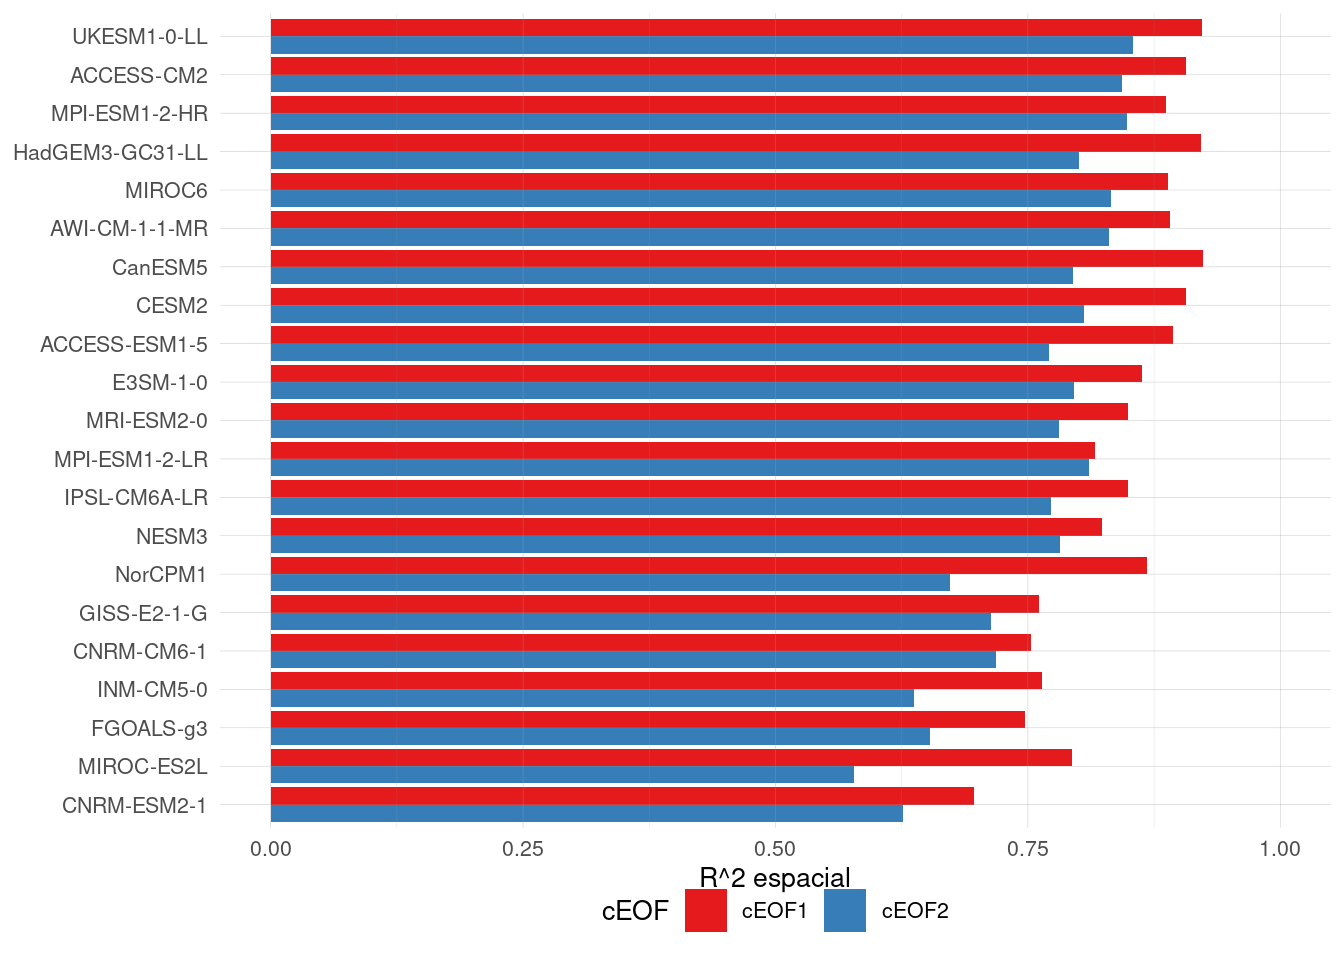
\includegraphics{figures/50-cmip6/comparacion-r2-1} 

}

\caption{Coeficiente de determinación (\(r^2\)) de los patrones espaciales de cada modelo con ERA5 para el cEOF1 (rojo) y cEOF2 (azul).}\label{fig:comparacion-r2}
\end{figure}

\begin{figure}

{\centering 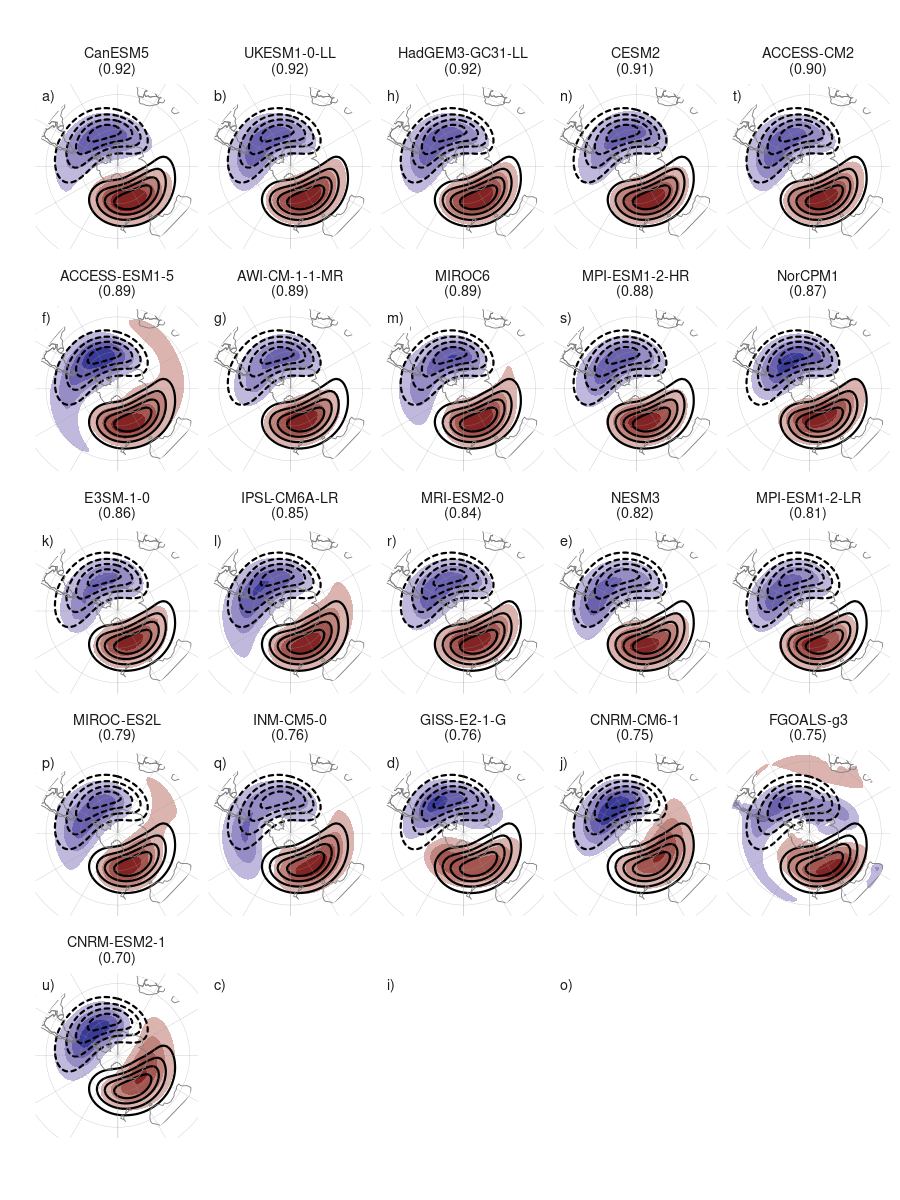
\includegraphics{figures/50-cmip6/todos-ceof1-1} 

}

\caption{Fase de 0º del cEOF1 en 50 hPa (sombreado, valores positivos en rojo, negativos en azul) de las corridas históricas de los modelos de CMIP6 analizados. Los contornos marcan el patrón de ERA5 (valores positivos en líneas llenas, valores negativos en línea punteada). Unidades arbitrarias.}\label{fig:todos-ceof1}
\end{figure}



\begin{figure}

{\centering \includegraphics{figures/50-cmip6/todos-ceof2-1} 

}

\caption{Igual que la Figura \ref{fig:todos-ceof1} pero para el cEOF2 en 200 hPa.}\label{fig:todos-ceof2}
\end{figure}



Para entender mejor los patrones espaciales representados por cada uno de los modelos, las Figuras \ref{fig:todos-ceof1} y \ref{fig:todos-ceof2} muestran la fase de 0º del cEOF1 y cEOF2, respectivamente, con los modelos ordenados de acuerdo al \(r^2\) del respectivo cEOF y los representados por ERA5.
Para el cEOF1 (Fig. \ref{fig:todos-ceof1}) todo los modelos excepto FGOALS-g3 (panel t) capturan correctamente el patrón de onda 1 observado.
Las diferencias con ERA5 son mínimas visualmente, como es de esperarse por la alta correlación espacial de estos patrones.
Para el cEOF2 (Fig. \ref{fig:todos-ceof2}), todos los modelos capturan el patrón de onda 3 localizado en el sector Pacífico-Atlántico.
En particular, el centro positivo al sur de Sudamérica y los centros negativos a los lados del mismo coinciden en todos los modelos con los centros de ERA5.
La principal característica de los modelos con baja correlación es la menor intensidad y mala localización del máximo localizado al sur de Nueva Zelanda.

El patrón medio multimodelo de la fase de cada cEOF en cada nivel, calculado promediando el patrón espacial correspondiente a cada uno de los modelos se muestra en la Figura \ref{fig:mmm}, junto con el \(r^2\) de estos patrones con respecto a los observados.
Los patrones son extremadamente similares a los observados en ERA5 y tienen \(r^2\) de 94\% y 89\% para el cEOF1 y el cEOF2 respectivamente.
La media multimodelo es más similar a los patrones observados que cualquier modelo individual, indicando que las deficiencias de cada modelo se compensan al promediar.

\begin{figure}

{\centering \includegraphics{figures/50-cmip6/mmm-1} 

}

\caption{Media multimodelo (sombreado, valores positivos en rojo, negativos en azul) de los campos espaciales de cada cEOF, fase y nivel. Los contornos marcan los patrones de ERA5 (valores positivos en líneas llenas, valores negativos en línea punteada). El \(r^2\) entre ERA5 y la media multimodelo está entre paréntesis. Unidades arbitrarias.}\label{fig:mmm}
\end{figure}



Los modelos del CMIP6 capturan entonces satisfactoriamente los patrones espaciales de los cEOFs, tanto en la media multimodelo como los modelos individuales.
Lo siguiente es explorar si los modelos logran capturar características de segundo orden, como su variabilidad y relación con otras partes del sistema climático.

\hypertarget{relaciuxf3n-con-la-variabilidad-tropical}{%
\subsection{Relación con la variabilidad tropical}\label{relaciuxf3n-con-la-variabilidad-tropical}}

Como se mostró en la Sección \ref{fuentes-ceof}, el cEOF2 está fuertemente relacionado con la variabilidad tropical.
Una primera aproximación para explorar esta relación en los modelos del CMIP6 fue calcular la correlación entre el cEOF2 y el ONI de cada modelo (Figura \ref{fig:cor-enso-plot}).
Se encontró que casi todos los modelos tienen una correlación alta entre el ONI y la fase de 90º del cEOF2 y casi nula correlación entre el ONI y la fase de 0º del cEOF2, lo cual es consistente con las observaciones.
Sin embargo, existe una gran variabilidad en la capacidad de los modelos de capturar esta relación.
Algunos, como MIROC6 y CESM2 tienen una correlación cercana a la observada, pero en la mayoría es mucho menor.
IPSL-CM6A-LR y INM-CM5-0 virtualmente no muestran relación entre el cEOF2 y el ONI.




\begin{figure}

{\centering \includegraphics{figures/50-cmip6/cor-enso-plot-1} 

}

\caption{Coeficiente de determinación (\(r^2\)) entre el índice ONI y las fases de 0º (azul)
y 90º (rojo) del cEOF2 para cada modelo del CMIP6 y para ERA5.}\label{fig:cor-enso-plot}
\end{figure}

\begin{figure}

{\centering \includegraphics{figures/50-cmip6/enso-phase-cmip-1} 

}

\caption{Valores del ONI en SON y la fase del cEOF2 para los modelos del CMIP6 en el período 1979--2014 y para ERA5 en el período 1979--2020. La línea negra representa el ajuste ONI \textasciitilde{} sen(fase) computado por cuadrados mínimos pesados por la magnitud del cEOF2 de forma equivalente a la Figura \ref{fig:enso-phase}.}\label{fig:enso-phase-cmip}
\end{figure}



\begin{figure}

{\centering \includegraphics{figures/50-cmip6/arg-enso-density-1} 

}

\caption{Estimación de densidad por núcleos de la fase del cEOF2 para primaveras con ONI menor a -0,5 (verde), entre -0,5 y 0,5 (naranja), y mayor a 0,5 (azul) para los modelos del CMIP6 en el período 1979--2014 y para ERA5 en el período 1979--2020.}\label{fig:arg-enso-density}
\end{figure}



La relación entre el cEOF2 y el ENSO se explica por una preferencia de fase cuando el forzante tropical está activo.
Para evaluar esto en los modelos del CMIP6, la Figura \ref{fig:enso-phase-cmip} muestra la relación entre el ENSO y la fase del cEOF2 para los modelos del CMIP6 y la Figura \ref{fig:arg-enso-density} la distribución de fases del cEOF2 para primaveras con ONI menor a -0,5, mayor a 0,5 y valores intermedios.
Los modelos con una correlación alta entre el cEOF2 y el ENSO muestran una relación sinusoidal fuerte, mientras que en los modelos con baja correlación la relación es más chata.
Las distribuciones de las fases según categorías del índice ONI (Fig. \ref{fig:arg-enso-density}) se ven bien separadas en las observaciones y en los modelos con alta correlación entre el cEOF2 y el ONI.
En estos modelos (ej. MIROC6, CESM2), cuando el ENSO está activo (definido como ONI \textgreater{} 0,5 o ONI \textless{} -0,5), la fase del cEOF2 se concentra cerca de \(\pm\) 90º (dependiendo del signo del ONI) mientras que cuando el ENSO no está tan activo (definido como ONI entre -0,5 y 0,5), la distribución de la fase es más uniforme.
En los modelos con baja correlación entre cEOF2 y ONI (ej. IPSL-CM6A-LR, INM-CM5-0) la distribución de fase es uniforme independientemente de la actividad del ENSO.

\begin{figure}

{\centering \includegraphics{figures/50-cmip6/fft-ceof2-1} 

}

\caption{Espectros de Fourier en cada modelo para la fase de 90º del cEOF2 (naranja), para la fase de 0º del cEOF2 (violeta) y para el ONI (negro). En línea obscura es el espectro promedio de todos los miembros, que se muestran en líneas translúcidas. El espectro del ONI es el espectro promedio de todos los miembros de cada modelo. Los paneles están ordenados de mayor a menor según el \(r^2\) entre la fase de 90º del cEOF2 y el ONI, el cual se muestra entre paréntesis en el título de cada panel.}\label{fig:fft-ceof2}
\end{figure}



La relación entre el cEOF2 y el ENSO también se evidencia en la similitud del periodograma de las series.
La Figura \ref{fig:fft-ceof2} muestra el periodograma para el cEOF2 con una línea por miembro y una línea gruesa marcando el periodograma promedio, así como el periodograma promedio del ONI de cada modelo.
La mayoría de los modelos tiene una periodicidad del ONI de \textasciitilde3 años similar a la observada en ERA5, aunque la intensidad y período máximo varía significativamente.

Todos los modelos que tienen una periodicidad clara en \textasciitilde3 años en la fase de 90º del cEOF2 también tienen una periodicidad del ENSO muy clara y además tienden a tener una correlación entre la fase de 90º del cEOF2 y el ENSO más alta.
Por otro lado, ninguno de los modelos con muy baja correlación con el ENSO pero periodicidad del ENSO clara presenta periodicidad clara en el cEOF2.

Sin embargo existen modelos con periodicidad del ENSO clara y correlación relativamente alta que no tienen periodicidad del cEOF2 clara.
MRI-ENSM2-0, UKESM1-0-LL, MPI-ESM1-2-LR son algunos ejemplos.

Estas observaciones sugieren que el ENSO es la fuente de periodicidad del cEOF2 en los modelos del CMIP6 pero que su capacidad para representar la periodicidad observada no sólo depende de la periodicidad del ENSO y del grado de correlación entre los índices.



\begin{figure}

{\centering \includegraphics{figures/50-cmip6/sst-mmm-1} 

}

\caption{Media multimodelo de regresión de la TSM con las fases de 0º y 90º de cada cEOF (K). El área sombreada muestra las zonas donde más de la mitad de los modelos tienen p-valor menor a 0,01. Los contornos negros muestran la regresión de TSM observada en ERA5.}\label{fig:sst-mmm}
\end{figure}

Para estudiar más en detalle esa relación, se evaluó la relación entre los cEOF y las anomalías de TSM.
La Figura \ref{fig:sst-mmm} muestra la media multimodelo de la regresión entre TSM y las dos fases de cada cEOF, marcando las zonas donde más de la mitad de los modelos tienen p-valores menores a 0,01.
Los modelos del CMIP6 reproducen los patrones de regresión de la fase de 90º del cEOF2 relativamente bien.
Se observa un exceso de señal en el Pacífico ecuatorial en la fase de 0º del cEOF2 que probablemente se deba a que estos modos no están alineados para minimizar esta relación.
Por otro lado, la señal asociada a la fase de 90º del cEOF1 sí muestra valores excesivamente altos no observados en ERA5.



\begin{figure}

{\centering \includegraphics{figures/50-cmip6/cor-sst-regr-1} 

}

\caption{Coeficiente de determinación (\(r^2\)) entre los patrones de regresión de las fases de 0º (violeta) y 90º (naranja) de cada cEOF y la TSM cada modelo y el patrón de regresión respectivo de ERA5.}\label{fig:cor-sst-regr}
\end{figure}

Para tener una visión global y cuantitativa de esta comparación, la Figura \ref{fig:cor-sst-regr} muestra el \(r^2\) entre las regresiones de TSM asociada con la fase de 90º del cEOF2 para cada modelo y la correspondiente regresión para ERA5.
En la mayoría de los modelos el patrón es similar al observado, excepto por INM-CM5-0.
Las regresiones asociadas con la fase de 0º del cEOF2, en cambio, tienen baja similitud con el observado en casi todos los modelos.
Posiblemente esto se deba al exceso de señal presente en la región del ENSO.

\hypertarget{relaciuxf3n-con-el-sam}{%
\subsection{Relación con el SAM}\label{relaciuxf3n-con-el-sam}}

En la Sección \ref{sam-ceof} se mostró que existía una relación importante entre las distintas fases de los cEOFs y las distintas componentes del SAM.
La Figura \ref{fig:cor-sam-cmip6} muestra el \(r^2\) entre las componentes del SAM y las fases de los cEOFs para los modelos del CMIP6.
Las líneas translúcidas son los valores para cada modelo y las áreas llenas representan el promedio multimodelo y su intervalo de confianza del 95\%; la línea gruesa corresponde al valor de ERA5.

\begin{figure}

{\centering \includegraphics{figures/50-cmip6/cor-sam-cmip6-1} 

}

\caption{Coeficiente de determinación (\(r^2\)) entre la fase de 0º (columna a y c) y 90º (columna b y d) de los cEOFs con el SAM (fila 1), A-SAM (fila 2) y S-SAM (fila 3) para cada nivel. Las líneas translúcidas son los valores promedio de cada modelo y las áreas llenas representan el promedio multimodelo y su intervalo de confianza del 95\%. La línea gruesa es el valor de ERA5. Equivalente a la Figura \ref{fig:sam-eof-vertical}.}\label{fig:cor-sam-cmip6}
\end{figure}



Se encuentra que la relación entre el cEOF1 y el SAM en los modelos del CMIP6 es similar a la observada, aunque con diferencias en la magnitud.

En cuanto al cEOF2, los modelos del CMIP6 capturan correctamente la falta de correlación entre fase de 0º del cEOF2 y el SAM y el S-SAM (paneles c.1 y c.3), pero tienen un nivel de correlación más alto de lo esperado con el A-SAM en la tropósfera (panel c.2).
La fase de 90º, en cambio, no muestra la relación observada con el SAM en la tropósfera (panel d.1).
A pesar de esto, sí tiene una relación alta con el A-SAM (panel d.2).
Esto implícitamente sugiere que los modelos CMIP6 no capturan correctamente la relación entre el PSA2 y el SAM, pero esta relación sí aparece si se filtra sólo la variabilidad de la parte asimétrica del SAM.

\hypertarget{tendencias}{%
\section{Tendencias}\label{tendencias}}

De la sección anterior surge que los modelos del CMIP6 logran capturar la estructura espacial de los cEOFs correctamente y que algunos modelos capturan también su variabilidad y relación con otras componentes del sistema climático.

En esta sección, se utilizaron las corridas largas de estos modelos y los experimentos de DAMIP para estudiar las tendencias a largo plazo y sus posibles forzantes.
Para extender las series temporales para todo el período disponible en CMIP6 y DAMIP, se proyectaron los campos espaciales de los dos cEOFs del período 1979--2014 en los campos desde 1850 hasta 2014.

\begin{figure}

{\centering \includegraphics{figures/50-cmip6/regresion-hgt-damip-1} 

}

\caption{Regresión de anomalías de altura geopotencial (m) con la fase de 0º (columna 1) y de 90º (columna 2) del cEOF1 en 50 hPa para el período 1940--2014 para los experimentos de CMIP6 y DAMIP.}\label{fig:regresion-hgt-damip}
\end{figure}



Los patrones espaciales de ambos cEOFs son muy similares en todos los experimentos y comparables con lo observado en la Figura \ref{fig:mmm} (no se muestra).
La regresión con la altura geopotencial, en cambio, tiene diferencias en el caso del cEOF1.
Estas regresiones se muestran en la Figura \ref{fig:regresion-hgt-damip} para el nivel de 50 hPa.
Si bien la localización general de los máximos es similar en todos los experimentos, en el experimento historical, la fase de 0º está asociada a una onda 1 mientras que la fase de 90º está asociada un monopolo con el centro sobre la Antártida oriental (Fig. \ref{fig:regresion-hgt-damip} fila a).
Esto es lo contrario de lo observado en ERA5, donde la fase de 0º era la asociada a una estructura más zonalmente simétrica (Fig. \ref{fig:eof1-regr-gh}).
Esto ocurre también para el experimento hist-stratO3, aunque en la fase 90 se observa mas bien una onda 1 que un monopolo (Fig \ref{fig:regresion-hgt-damip}, fila c).
Por otra parte, las regresiones para el experimento hist-aer (Fig. \ref{fig:regresion-hgt-damip} fila e) son mas similares a las observadas, así como aquellas para el experimento hist-GHG (Fig. \ref{fig:regresion-hgt-damip} fila b) y en menor medida para el experimento hist-nat (Fig. \ref{fig:regresion-hgt-damip}, fila d).

\begin{figure}

{\centering \includegraphics{figures/50-cmip6/series-largas-1} 

}

\caption{Series temporales de anomalías estandarizadas de los cEOFs computados usando el período 1850 -- 2014 promediadas para cada modelo (líneas translúcidas) y su media multimodelo (línea oscura). Las anomalías están computadas con respecto a la media entre 1850 y 1900. En líneas translúcidas se muestran las series de cada modelo.}\label{fig:series-largas}
\end{figure}



La Figura \ref{fig:series-largas} muestra las series temporales durante todo el período.
La fase de 0º del cEOF1 tiene una pequeña tendencia positiva comenzando alrededor de 1940, consistente con la tendencia observada en ERA5 (Fig. \ref{fig:extended-series}).
Sin embargo, la fase de 90º del cEOF1 tiene una tendencia negativa mucho mayor, la cual no está presente en ERA5.

\begin{figure}

{\centering \includegraphics{figures/50-cmip6/trends-ceof1-1} 

}

\caption{Tendencias lineales de cada fase del cEOF1 desde 1940. Cada punto representa un miembro, donde los miembros con tendencias significativas (p-valor \textless{} 0,01) se marcan con una cruz. La línea vertical punteada representa la tendencia media de todos los modelos.}\label{fig:trends-ceof1}
\end{figure}



Las tendencias de cada fase del cEOF1 para cada modelo desde 1940 se muestran en la Figura \ref{fig:trends-ceof1} junto con la tendencia promedio de todos los modelos.
La tendencia media de la fase de 0º es positiva pero muy pequeña.
Además, los modelos no son consistentes en sus tendencias y sólo algunos modelos tienen una tendencia promedio positiva.
Por otro lado, las tendencias de la fase de 90º son más consistentes.

Estas tendencias son incompatibles con la variabilidad del cEOF1 observado, el cual tiene una tendencia positiva de su fase de 0º y ninguna tendencia en su fase de 90º.
Es posible que los modelos tengan algún problema fundamental al capturar la variabilidad a largo plazo de este modo, ya sea por falencias en la dinámica interna o por algún problema con el forzante involucrado.

También es posible que la tendencia observada se deba a variabilidad interna de baja frecuencia.
En este caso, no sería esperable que los modelos capturen correctamente la fase de esta variabilidad, por lo que no sería observable ni en la media multimodelo ni en las tendencias de cada miembro particularmente en el período 1940--2014.
ERA5 puede considerarse como una realización particular del ensamble climático y es posible que la tendencia particular observada no sea necesariamente representativa del forzante externo.

Alternativamente, dado que el cEOF1 captura el campo medio de las anomalías zonales de altura geopotencial y que los distintos modelos de CMIP6 tienen potencialmente un campo medio distinto a ERA5, es posible que la rotación elegida del cEOF1 no sea la ideal para capturar la variabilidad de largo plazo compatible con lo observado en ERA5.

La Figura \ref{fig:ceof-damip} muestra las series temporales para los experimentos hist-GHG, hist-nat, hist-stratO3 e hist-aer junto al experimento histórico y la Figura \ref{fig:mapa-trend} muestra las tendencias de la altura geopotencial en 50 hPa que son explicadas por cada fase del cEOF1 y la suma de ambas.
Esto se calculó como el valor de la regresión lineal entre cada fase del cEOF1 y la altura geopotencial multiplicado por la tendencia lineal de cada fase del cEOF1.
En estas figuras se excluyen los experimentos hist-nat e hist-aer ya que sus tendencias son poco significativas.

\begin{figure}

{\centering \includegraphics{figures/50-cmip6/ceof-damip-1} 

}

\caption{Igual que la Figura \ref{fig:series-largas} pero para cada experimento de DAMIP y el experimento histórico en negro.}\label{fig:ceof-damip}
\end{figure}



\begin{figure}

{\centering \includegraphics{figures/50-cmip6/mapa-trend-1} 

}

\caption{Tendencias de altura geopotencial (m por decada) en 50 hPa concordante con la tendencia de la fase de 0º y 90º del cEOF1 y su suma.}\label{fig:mapa-trend}
\end{figure}



La fase de 90º del cEOF1, presenta una tendencia positiva en hist-aer y negativa en hist-GHG y, también negativa pero más débil, en hist-stratO3.
La disminución del ozono estratosférico y el aumento de las concentraciones de GHG contribuyen a la tendencia negativa.
Ambos efectos tienden a reducir la altura geopotencial en 50 hPa sobre la Antártida oriental (Fig. \ref{fig:mapa-trend} columna 2).
Este efecto combinado de ambos forzantes ha sido ya identificada por trabajos previos como aquella que mayormente explica la intensificación y progresión hacia el polo de los vientos del oeste (\protect\hyperlink{ref-ipcc6ch3}{Intergovernmental Panel on Climate Change (IPCC), 2023}).

Para la fase de 0º del cEOF1, ni hist-nat ni hist-aer muestran tendencias significativas, sugiriendo que la tendencia observada no se debe a variabilidad ni al forzante de los aerosoles antropogénicos.
Por otro lado, hist-stratO3 muestra una tendencia mucho mayor a la observada e hist-GHG muestra una tendencia negativa de similar magnitud la de hist-stratO3.
Esto sugiere que el ozono estratosférico y los gases de efecto invernadero tienen efectos contrarios sobre esta fase del cEOF1.

El efecto de la tendencia de la fase de 0º del cEOF1 en el experimento hist-GHG en la altura geopotencial de 50 hPa es una leve anomalía negativa sobre el Mar de Ross (Fig. \ref{fig:mapa-trend} b.1).
Este patrón indicaría un aumento del jet al Sur de Nueva Zelanda.
Este efecto es opuesto al efecto en el experimento hist-stratO3



\begin{figure}

{\centering \includegraphics{figures/50-cmip6/suma-1} 

}

\caption{Media multimodelo de las series temporales estandarizadas de las fases de 0º y 90º del cEOF1 para el experimento historical (azul) y para la suma de los experimentos hist-GHG, hist-stratO3 e hist-aer, es decir, los que consideran cambios antropogénicos (rojo). La líneas gruesas indican un suavizado usado regresión local.}\label{fig:suma}
\end{figure}

Como una primera aproximación al efecto combinado de todos estos forzantes, la Figura \ref{fig:suma} muestra la media multimodelo de la corrida histórica junto con la suma de las medias multimodelo de las corridas hist-GHG, hist-stratO3 e hist-aer.
Ambas series presentan una tendencia a largo plazo virtualmente idéntica, sugiriendo que el efecto de los forzantes es aproximadamente lineal.

\hypertarget{conclusiones-del-capuxedtulo-refcmip6}{%
\section{Conclusiones del capítulo \ref{cmip6}}\label{conclusiones-del-capuxedtulo-refcmip6}}

Los modelos del CMIP6 consiguen caracterizar la estructura espacial de los cEOFs satisfactoriamente, con una buena correlación entre los patrones espaciales, particularmente para la media multimodelo.
La habilidad de los modelos de capturar sus características de segundo orden, como la relación con el ENSO y el SAM no es tan buena ni homogénea entre modelos.
Sólo algunos modelos, como MIROC6 y CESM2 consiguen capturar con todas sus características la influencia del ENSO en la fase del cEOF2 y la relación de la mayoría de los modelos con el SAM es menor a la observada.

La tendencia levemente positiva de la fase de 0º del cEOF1 es capturada por la media multimodelo y el análisis de las corridas de DAMIP indican que está principalmente asociada por el forzarte del ozono estratosférico parcialmente compensado por el forzante de los gases de efecto invernadero.
Los modelos del CMIP6 también presentan una tendencia negativa importante en la fase de 90º del cEOF1 no presente en las observaciones que la asocian con el forzante de gases de efecto invernadero principalmente y en menor medida con el forzante del ozono y compensados con el forzante de los aerosoles.

\hypertarget{conclusiones}{%
\chapter{Conclusiones}\label{conclusiones}}

Esta tesis se propuso mejorar el entendimiento de las asimetrías zonales de la circulación extratropical del hemisferio sur.

Se comenzó evaluando las formas tradicionales de describir estas asimetrías, que son principalmente a través del análisis del patrón de onda 3 como lo propuso M. N. Raphael (\protect\hyperlink{ref-raphael2004}{2004}) o a través de un análisis de Fourier.
Sin embargo, se encontró que estos métodos no son capaces de caracterizar propiedades importantes de la circulación asimétrica, como su dispersión meridional, la amplitud variable de los centros que la caracterizan a lo largo de cada círculo de latitud y la variación de su fase a lo largo del año.

Considerando estas limitaciones, esta tesis propuso una forma alternativa para la caracterización de la circulación zonalmente asimétrica del hemisferio sur a partir del uso de Funciones Empíricas Ortogonales Complejas (cEOF), metodología que permite capturar oscilaciones con amplitud y fase variables.
Dada la alta correlación temporal entre los modos observados en la tropósfera y estratósfera y la similitud de sus patrones espaciales al aplicar la metodología cEOF en distintos niveles atmosféricos, se consideró que pueden tratarse como modos de variabilidad conjunta.
Por lo tanto, los cEOF se calcularon utilizando la altura geopotencial de los niveles de 200 hPa y 50 hPa en conjunto.
Se hizo foco en la estación de primavera, ya que durante ésta se maximizan las teleconexiones entre los trópicos y extratrópicos.

El primer modo obtenido a partir del análisis cEOF (cEOF1) representa un patrón de onda 1 y es principalmente un modo estratosférico con fuerte asociación con la dinámica del vórtice polar.
La regresión de las anomalías temporales de altura geopotencial con este modo tanto en su fase 0 como en su fase 90 muestran su influencia significativa en modular la ubicación e intensidad del centro de anomalía sobre la región antártica en asociación con un centro y banda de anomalías de signo opuesto en latitudes medias.
Acorde, este modo presenta una correlación significativa con la actividad del SAM como se discute más abajo.
En especial se encontró que presenta una asociación significativa con las anomalías de Columna Total de Ozono, lo cual es también otra evidencia de la influencia de la dinámica estratosférica en el comportamiento de este modo.
Por otra parte, no presenta asociación significativa con fuentes de variabilidad tropical.
En superficie, no presenta influencia significativa en la precipitación.
Sí, en cambio, influye significativamente en las anomalías de la temperatura del aire en superficie en Antártida Occidental y en especial en la Península Antártica, así como en algunas regiones oceánicas en la vecindad de Australia, Sudamérica y África.
Esto es coherente con trabajos previos que confirman la influencia del SAM sobre las anomalías de temperatura regionales en el hemisferio sur.

El segundo modo obtenido a partir del análisis cEOF (cEOF2) representa una estructura espacial de onda 3 que está localizado principalmente en el sector del océano Pacífico.
Se encontró que está fuertemente asociado con trenes de onda del tipo PSA.
Además, es una forma alternativa de representar a los modos PSA1 y PSA2 (que surgen del tradicional análisis de EOF) como un único modo conjunto con una amplitud y una fase continua.
Al igual que el cEOF1, este segundo modo presenta vinculación con el SAM, pero a diferencia del primer modo, la variabilidad del cEOF2 está fuertemente influenciada por la variabilidad tropical.
Además se mostró que el cEOF2 surge como un modo de variabilidad interna de la atmósfera extratropical, aunque en ausencia del forzante tropical carece de una fase preferencial.
El forzante tropical no influye significativamente en su intensidad, pero sí tiende a determinar una fase estacionaria.
Esto es consistente con Cai and Watterson (\protect\hyperlink{ref-cai2002}{2002}), quienes encontraron a partir de simulaciones con un modelo de circulación general acoplado que se puede desarrollar actividad tipo PSA aún con condiciones medias climatológicas en el océano superficial, removiendo la variabilidad de tipo ENSO, pero que la actividad de uno de los modos PSA se incrementa al incluirla.

Consistente con su relación con el ENSO, los impactos del cEOF2 en la superficie son significativos y dependientes de su fase.
En los extratrópicos, la fase de 90º se asocia con anomalías positivas de precipitación en el SESA y negativas en Australia en patrones consistentes con la señal del ENSO en la precipitación.
También se observaron anomalías significativas de temperatura en estos continentes y en la Antártida Occidental.

Se concluye entonces que el cEOF2 describe a la onda 3 de una manera matemática y físicamente más completa que la descripción que se obtiene con otros métodos previamente descritos.
Recientemente, Goyal et al. (\protect\hyperlink{ref-goyal2022}{2022}) propuso un índice alternativo para la onda 3 basado en los primeros dos EOF del viento meridional en 500 hPa.
Aunque este método tiene similitudes con el cEOF2, depende de la inspección visual, por lo que no garantiza que la construcción de la fase y la amplitud sea realmente válida.
En cambio, el cEOF2 tiene la ventaja de construirse como un patrón de ondas con amplitud y fase por construcción.

Los resultados obtenidos tanto con el cEOF1 como con el cEOF2 muestran en suma que ambos modos a través de sus fases y amplitudes variables proporcionan una descripción más profunda y compleja de las principales estructuras asociadas con la variabilidad de la circulación del hemisferio sur como son la estructura anular polar, la onda 3 extratropical y los trenes de onda extendidos desde el Indico-Pacífico tropical hacia Sudamérica, que aquella proporcionada por el método de EOF tradicional.
Esto abre nuevas oportunidades para estudiar desde un abordaje diferente la influencia, tanto de la variabilidad tropical como de la variabilidad estratosférica, en la circulación del hemisferio sur y en sus porciones continentales.

El análisis del comportamiento asimétrico de la circulación del hemisferio sur se completó con el estudio de las características simétricas y asimétricas del SAM, por ser el patrón principal que explica su variabilidad temporal.
Para esto se desarrollaron índices para describir la componente simétrica del SAM (S-SAM) y la componente asimétrica del SAM (A-SAM), a partir de la media zonal y de las anomalías espaciales del SAM completo .

Tanto en la estratosfera como en la tropósfera, la estructura de las anomalías temporales de la altura geopotencial asociados al S-SAM es mucho más anular que aquella asociada con el SAM completo.
Por otro lado, el índice A-SAM está asociado en la estratosfera a un patrón de onda 1 y en la troposfera a un patrón de onda 3 con amplitud máxima en el pacífico muy similar a la fase de 90º del cEOF2.

La correlación significativa entre el índice SAM y el ENSO es capturada en su totalidad por el A-SAM, lo que sugiere que el ENSO y el SAM están conectados únicamente por la variabilidad zonalmente asimétrica.
El A-SAM es, por lo tanto, una medida muy útil para estudiar la relación entre estos dos modos de variabilidad.
Por otro lado, este resultado abre la pregunta sobre si la componente asimétrica del SAM forma parte intrínsicamente de este modo interno de variabilidad, o es en cambio un reflejo de la influencia del ENSO en la circulación extratropical que por construcción queda embebido en el primer EOF aplicado a las anomalías temporales.
Evidencias de esta posibilidad se encuentran en el antiguo trabajo de Kidson (\protect\hyperlink{ref-kidson1988}{1988}) donde, aplicando rotación a las EOFs, obtiene modos rotados que separan una estructura anular similar a la obtenida con el S-SAM de un patrón de onda 3 similar al obtenido con el A-SAM.
Estudios futuros deberían abordar esta cuestión con mayor profundidad.

El análisis de las tendencias positivas del SAM de verano y otoño en la troposfera entre 1940 y 2020, que fueron identificadas como significativas por estudios previos (p.ej. \protect\hyperlink{ref-fogt2020}{Fogt and Marshall, 2020} y sus referencias) son únicamente explicadas por la tendencia del S-SAM.
También se dedectó una tendencia positiva estadísticamente significativa en el S-SAM en la estratósfera en otoño que no es evidente en el índice SAM.
Hay evidencia de que el SAM está evolucionando hacia ser más asimétrico en verano, aunque el período es corto y la señal no es muy robusta.
Esto es contrario a lo observado por Fogt et al. (\protect\hyperlink{ref-fogt2012}{2012}), aunque la discrepancia puede deberse a las diferencias metodológicas o al período analizado.

La fase positiva del SAM está asociado, a grandes rasgos, con anomalías de temperatura negativas en latitudes polares rodeadas de anomalías de temperatura positivas en latitudes más bajas.
Entre otoño y primavera el S-SAM está principalmente asociado con anomalías de temperatura negativas sobre el continente antártico (principalmente en Antártida oriental) y positivas sobre la Península Antártica, y con anomalías negativas en el Pacífico Sur.
El índice A-SAM describe principalmente en el sector del Pacífico Sur hasta la costa antártica una alternancia de anomalías de temperatura de signos contrapuestos que son coherentes con la onda 3 que describe las anomalías de altura geopotencial.

Asimismo, tanto en Sudamérica como en Australia, las anomalías de precipitación asociadas al SAM mezclan las contribuciones del S-SAM y del A-SAM, las cuales responden a distintos procesos físicos.
En el sur de Chile, las anomalías negativas de precipitación asociadas al SAM se explican por el desplazamiento de los oestes hacia el Sur asociado al S-SAM.
En el SESA, en cambio, las anomalías negativas de precipitación asociadas al SAM se explican por el efecto del anticiclón en el Atlántico Sur asociado al A-SAM.~

En relación a la vinculación de la componentes del SAM con los cEOFs se encontró que la relación entre el SAM y el cEOF1 está explicada en su totalidad por la componente S-SAM mientras que la relación entre el SAM y la fase de 90º del cEOF2 es explicada principalmente por el A-SAM.
Esto nuevamente confirma que la descripción de la circulación en términos de su componente simétrica y asimétrica proporciona un mayor detalle de los procesos que caracterizan su asociación con el SAM.
Asimismo, la fuerte correlación entre el A-SAM y la fase 90 del cEOF2 es otra evidencia de la importante influencia del ENSO en la estructura de onda 3 a través de las teleconexiones del tipo PSA.,

Al evaluar la capacidad de los modelos del CMIP6 para describir los patrones cEOF, se encontró que los 19 modelos analizados capturan correctamente la estructura espacial de los cEOFs, pero no todos consiguen capturar su variabilidad temporal y relaciones con otras variables climáticas.
Por otra parte, la relación entre la fase de 90º del cEOF2 y el SAM no está presente en la mayoría de los modelos, pero sí la relación con el A-SAM, aunque en menor medida.

Se detectó una leve tendencia positiva en la fase de 0º del cEOF1 en ERA5 en el período 1940--2022.
Ésta no es simulada consistentemente por los modelos de CMIP6; la media multimodelo presenta una tendencia positiva pero de baja magnitud.
Por otro lado, aparece en los modelos una tendencia negativa mucho más intensa en la fase de 90º que no está presente en las observaciones.
Los experimentos que consideran por separado los forzantes naturales y los distintos forzantes antropogénicos (gases de efecto invernadero, ozono estratosférico, aerosoles) sugieren que los gases de efecto invernadero contribuyen a una tendencia negativa en ambas fases, mientras que la variación del ozono estratosférico aporta a una tendencia positiva en la fase de 0º de modo que compensa el efecto de los gases de efecto invernadero y generan una tendencia neta positiva.

Entre las causas que explican las diferencias entre las tendencias observadas y simuladas se puede mencionar una incorrecta sensibilidad a los forzantes en los modelos, problemas de la capacidad de los modelos para resolver procesos clave en la dinámica de la circulación asimétrica zonal del hemisferio sur como la variabilidad del vórtice polar, el agujero en la capa de ozono, o a diferencias en los campos medios de anomalías zonales de geopotencial.
Finalmente, dado que ERA5 es sólo una realización del sistema climático, no se puede descartar que las tendencias representadas por la media multimodelo de los modelos de CMIP6 sean una mejor representación de los efectos de los forzantes.

En resumen, este trabajo de tesis aporta nuevas herramientas para mejorar el entendimiento de la circulación zonalmente asimétrica del hemisferio sur al analizar los principales patrones de circulación mediante cEOFs y al estudiar por separado las componentes zonalmente asimétricas y simétricas del SAM.

El cEOF principal es un patrón de onda 1 vinculado al vórtice polar, al SAM y a las anomalías de ozono que tiene impacto sobre la temperatura en la Antártida.
Por otro lado, el segundo cEOF está asociado a la onda zonal 3 y describe el patrón de teleconexiones entre los trópicos y los extratrópicos.
Los modelos de CMIP6 se mostraron adecuados para representar estos modos pero no todos consiguen simular su relación con el ENSO o el SAM ni sus tendencias correctamente.

Tomados en su conjunto, estos patrones permiten representar las características principales de la variabilidad del hemisferio sur.
La variabilidad anular con el S-SAM, el vórtice polar con el cEOF1 y los trenes de onda de Rossby con el cEOF2.

Estos resultados abren la puerta a muchas investigaciones futuras.
Es necesario extender el estudio a otros trimestres además de SON, así como adentrar en el impacto de estos modos en otras variables del sistema climático.
Queda pendiente estudiar en más detalle cómo se comporta el cEOF2 en ausencia de variabilidad tropical y cuál es su relación con la variabilidad del vórtice polar.
A su vez, quedan sin dilucidar los mecanismos que establecen la relación entre el S-SAM y el A-SAM/cEOF2, los cuales pueden ser estudiados mediante simulaciones de sensibilidad.
En cuanto a los modelos de CMIP6, un estudio más detallado de las propiedades de cada modelo podría permitir entender qué procesos son importantes para una correcta caracterización de la circulación asimétrica y sus tendencias.

\backmatter

\hypertarget{referencias}{%
\chapter*{Referencias}\label{referencias}}
\addcontentsline{toc}{chapter}{Referencias}

\markboth{Referencias}{Referencias}

\noindent

\setlength{\parindent}{-0.20in}

\hypertarget{refs}{}
\begin{CSLReferences}{1}{0}
\leavevmode\vadjust pre{\hypertarget{ref-fishpack}{}}%
Adams, J. C., Swartztrauber, P. N. and Sweet, R. (1999). \emph{{FISHPACK}, a package of {Fortran} subprograms for the solution of separable elliptic partial differential equations}. https://www2.cisl.ucar.edu/resources/legacy/fishpack.

\leavevmode\vadjust pre{\hypertarget{ref-albers2020}{}}%
Albers, S. and Campitelli, E. (2020). \emph{Rsoi: {Import Various Northern} and {Southern Hemisphere Climate Indices}}.

\leavevmode\vadjust pre{\hypertarget{ref-allaire2020}{}}%
Allaire, J. J., Xie {[}aut, Y., cre, McPherson, J., Luraschi, J., Ushey, K., Atkins, A., Wickham, H., Cheng, J., Chang, W., Iannone, R., Dunning, A., filter), A. Y. (Number. sections L., Schloerke, B., Dervieux, C., Aust, F., Allen, J., Seo, J., Barrett, M. \ldots{} filter), A. K. (pagebreak. L. (2020). \emph{Rmarkdown: {Dynamic Documents} for {R}}.

\leavevmode\vadjust pre{\hypertarget{ref-arblaster2006}{}}%
Arblaster, J. M. and Meehl, G. A. (2006). Contributions of {External Forcings} to {Southern Annular Mode Trends}. \emph{Journal of Climate}, \emph{19}(12), 2896--2905. \url{https://doi.org/10.1175/JCLI3774.1}

\leavevmode\vadjust pre{\hypertarget{ref-CMIP6.CMIP.E3SM-Project.E3SM-1-0}{}}%
Bader, D. C., Leung, R., Taylor, M. and McCoy, R. B. (2019). \emph{E3SM-project E3SM1.0 model output prepared for CMIP6 CMIP}. \url{https://doi.org/10.22033/ESGF/CMIP6.2294}

\leavevmode\vadjust pre{\hypertarget{ref-baldwin2001}{}}%
Baldwin, M. P. (2001). Annular modes in global daily surface pressure. \emph{Geophysical Research Letters}, \emph{28}(21), 4115--4118. \url{https://doi.org/10.1029/2001GL013564}

\leavevmode\vadjust pre{\hypertarget{ref-baldwin2001b}{}}%
Baldwin, M. P., Gray, L. J., Dunkerton, T. J., Hamilton, K., Haynes, P. H., Randel, W. J., Holton, J. R., Alexander, M. J., Hirota, I., Horinouchi, T., Jones, D. B. A., Kinnersley, J. S., Marquardt, C., Sato, K. and Takahashi, M. (2001). The quasi-biennial oscillation. \emph{Reviews of Geophysics}, \emph{39}(2), 179--229. \url{https://doi.org/10.1029/1999RG000073}

\leavevmode\vadjust pre{\hypertarget{ref-baldwin2009}{}}%
Baldwin, M. P. and Thompson, D. W. J. (2009). A critical comparison of stratosphere{\textendash}troposphere coupling indices. \emph{Quarterly Journal of the Royal Meteorological Society}, \emph{135}(644), 1661--1672. \url{https://doi.org/10.1002/qj.479}

\leavevmode\vadjust pre{\hypertarget{ref-bamston1997}{}}%
Bamston, A. G., Chelliah, M. and Goldenberg, S. B. (1997). Documentation of a highly {ENSO}-related sst region in the equatorial pacific: {Research} note. \emph{Atmosphere-Ocean}, \emph{35}(3), 367--383. \url{https://doi.org/10.1080/07055900.1997.9649597}

\leavevmode\vadjust pre{\hypertarget{ref-benjamini1995}{}}%
Benjamini, Y. and Hochberg, Y. (1995). Controlling the {False Discovery Rate}: {A Practical} and {Powerful Approach} to {Multiple Testing}. \emph{Journal of the Royal Statistical Society: Series B (Methodological)}, \emph{57}(1), 289--300. \url{https://doi.org/10.1111/j.2517-6161.1995.tb02031.x}

\leavevmode\vadjust pre{\hypertarget{ref-CMIP6.CMIP.NCC.NorCPM1}{}}%
Bethke, I., Wang, Y., Counillon, F., Kimmritz, M., Fransner, F., Samuelsen, A., Langehaug, H. R., Chiu, P.-G., Bentsen, M., Guo, C., Tjiputra, J., Kirkevåg, A., Oliviè, D. J. L., Seland, ?yvind., Fan, Y., Lawrence, P., Eldevik, T. and Keenlyside, N. (2019). \emph{NCC NorCPM1 model output prepared for CMIP6 CMIP}. \url{https://doi.org/10.22033/ESGF/CMIP6.10843}

\leavevmode\vadjust pre{\hypertarget{ref-CMIP6.CMIP.IPSL.IPSL-CM6A-LR}{}}%
Boucher, O., Denvil, S., Levavasseur, G., Cozic, A., Caubel, A., Foujols, M.-A., Meurdesoif, Y., Cadule, P., Devilliers, M., Ghattas, J., Lebas, N., Lurton, T., Mellul, L., Musat, I., Mignot, J. and Cheruy, F. (2018). \emph{IPSL IPSL-CM6A-LR model output prepared for CMIP6 CMIP}. \url{https://doi.org/10.22033/ESGF/CMIP6.1534}

\leavevmode\vadjust pre{\hypertarget{ref-CMIP6.DAMIP.IPSL.IPSL-CM6A-LR}{}}%
Boucher, O., Denvil, S., Levavasseur, G., Cozic, A., Caubel, A., Foujols, M.-A., Meurdesoif, Y. and Gastineau, G. (2018). \emph{IPSL IPSL-CM6A-LR model output prepared for CMIP6 DAMIP}. \url{https://doi.org/10.22033/ESGF/CMIP6.13801}

\leavevmode\vadjust pre{\hypertarget{ref-cai2020a}{}}%
Cai, W., McPhaden, M. J., Grimm, A. M., Rodrigues, R. R., Taschetto, A. S., Garreaud, R. D., Dewitte, B., Poveda, G., Ham, Y.-G., Santoso, A., Ng, B., Anderson, W., Wang, G., Geng, T., Jo, H.-S., Marengo, J. A., Alves, L. M., Osman, M., Li, S. \ldots{} Vera, C. (2020). Climate impacts of the {El Ni{ñ}o}{\textendash}{Southern Oscillation} on {South America}. \emph{Nature Reviews Earth \& Environment}, \emph{1}(4), 215--231. \url{https://doi.org/10.1038/s43017-020-0040-3}

\leavevmode\vadjust pre{\hypertarget{ref-cai2011}{}}%
Cai, W., Rensch, P. van, Cowan, T. and Hendon, H. H. (2011). Teleconnection {Pathways} of {ENSO} and the {IOD} and the {Mechanisms} for {Impacts} on {Australian Rainfall}. \emph{Journal of Climate}, \emph{24}(15), 3910--3923. \url{https://doi.org/10.1175/2011JCLI4129.1}

\leavevmode\vadjust pre{\hypertarget{ref-cai2002}{}}%
Cai, W. and Watterson, I. G. (2002). Modes of {Interannual Variability} of the {Southern Hemisphere Circulation Simulated} by the {CSIRO Climate Model}. \emph{Journal of Climate}, \emph{15}(10), 1159--1174. \url{https://doi.org/10.1175/1520-0442(2002)015\%3C1159:MOIVOT\%3E2.0.CO;2}

\leavevmode\vadjust pre{\hypertarget{ref-campitelli2020}{}}%
Campitelli, E. (2020). \emph{{metR}: {Tools} for {Easier Analysis} of {Meteorological Fields}}.

\leavevmode\vadjust pre{\hypertarget{ref-rcmip6}{}}%
Campitelli, E. (2023). \emph{Rcmip6}. Zenodo. \url{https://doi.org/10.5281/zenodo.10138834}

\leavevmode\vadjust pre{\hypertarget{ref-campitelli2018b}{}}%
Campitelli, E. (2018). \emph{{Estudio de los mecanismos f{í}sicos asociados con el patr{ó}n de onda 3 de la circulaci{ó}n atmosf{é}rica del Hemisferio Sur}} {[}\{Tesis de Licenciatura\}{]}. Universidad de Buenos Aires.

\leavevmode\vadjust pre{\hypertarget{ref-campitelli2022}{}}%
Campitelli, E., Díaz, L. B. and Vera, C. (2022). Assessment of zonally symmetric and asymmetric components of the {Southern Annular Mode} using a novel approach. \emph{Climate Dynamics}, \emph{58}(1), 161--178. \url{https://doi.org/10.1007/s00382-021-05896-5}

\leavevmode\vadjust pre{\hypertarget{ref-campitelli2023}{}}%
Campitelli, E., Díaz, L. B. and Vera, C. (2023). Revisiting the zonally asymmetric extratropical circulation of the {Southern Hemisphere} spring using complex empirical orthogonal functions. \emph{Climate Dynamics}. \url{https://doi.org/10.1007/s00382-023-06780-0}

\leavevmode\vadjust pre{\hypertarget{ref-CMIP6.CMIP.NUIST.NESM3}{}}%
Cao, J. and Wang, B. (2019). \emph{NUIST NESMv3 model output prepared for CMIP6 CMIP}. \url{https://doi.org/10.22033/ESGF/CMIP6.2021}

\leavevmode\vadjust pre{\hypertarget{ref-cazes-boezio2003}{}}%
Cazes-Boezio, G., Robertson, A. W. and Mechoso, C. R. (2003). Seasonal {Dependence} of {ENSO Teleconnections} over {South America} and {Relationships} with {Precipitation} in {Uruguay}. \emph{Journal of Climate}, \emph{16}(8), 1159--1176. \url{https://doi.org/10.1175/1520-0442(2003)16\%3C1159:SDOETO\%3E2.0.CO;2}

\leavevmode\vadjust pre{\hypertarget{ref-chung1999}{}}%
Chung, C. and Nigam, S. (1999). Weighting of geophysical data in {Principal Component Analysis}. \emph{Journal of Geophysical Research: Atmospheres}, \emph{104}(D14), 16925--16928. \url{https://doi.org/10.1029/1999JD900234}

\leavevmode\vadjust pre{\hypertarget{ref-clem2013}{}}%
Clem, K. R. and Fogt, R. L. (2013). Varying roles of {ENSO} and {SAM} on the {Antarctic Peninsula} climate in austral spring. \emph{Journal of Geophysical Research: Atmospheres}, \emph{118}(20), 11, 481--411, 492. \url{https://doi.org/10.1002/jgrd.50860}

\leavevmode\vadjust pre{\hypertarget{ref-CMIP6.CMIP.NCAR.CESM2}{}}%
Danabasoglu, G. (2019a). \emph{NCAR CESM2 model output prepared for CMIP6 CMIP}. \url{https://doi.org/10.22033/ESGF/CMIP6.2185}

\leavevmode\vadjust pre{\hypertarget{ref-CMIP6.DAMIP.NCAR.CESM2}{}}%
Danabasoglu, G. (2019b). \emph{NCAR CESM2 model output prepared for CMIP6 DAMIP}. \url{https://doi.org/10.22033/ESGF/CMIP6.2187}

\leavevmode\vadjust pre{\hypertarget{ref-CMIP6.CMIP.CSIRO-ARCCSS.ACCESS-CM2}{}}%
Dix, M., Bi, D., Dobrohotoff, P., Fiedler, R., Harman, I., Law, R., Mackallah, C., Marsland, S., O'Farrell, S., Rashid, H., Srbinovsky, J., Sullivan, A., Trenham, C., Vohralik, P., Watterson, I., Williams, G., Woodhouse, M., Bodman, R., Dias, F. B. \ldots{} Yang, R. (2019). \emph{CSIRO-ARCCSS ACCESS-CM2 model output prepared for CMIP6 CMIP}. \url{https://doi.org/10.22033/ESGF/CMIP6.2281}

\leavevmode\vadjust pre{\hypertarget{ref-CMIP6.DAMIP.CSIRO-ARCCSS.ACCESS-CM2}{}}%
Dix, M., Mackallah, C., Bi, D., Bodman, R., Marsland, S., Rashid, H., Woodhouse, M. and Druken, K. (2020). \emph{CSIRO-ARCCSS ACCESS-CM2 model output prepared for CMIP6 DAMIP}. \url{https://doi.org/10.22033/ESGF/CMIP6.14361}

\leavevmode\vadjust pre{\hypertarget{ref-dowle2020}{}}%
Dowle, M. and Srinivasan, A. (2020). \emph{Data.table: {Extension} of 'data.frame'}.

\leavevmode\vadjust pre{\hypertarget{ref-CMIP6.DAMIP.E3SM-Project.E3SM-1-0}{}}%
\emph{E3SM-project E3SM1.0 model output prepared for CMIP6 DAMIP}. (2022). \url{http://cera-www.dkrz.de/WDCC/meta/CMIP6/CMIP6.DAMIP.E3SM-Project.E3SM-1-0}

\leavevmode\vadjust pre{\hypertarget{ref-eyring2016}{}}%
Eyring, V., Bony, S., Meehl, G. A., Senior, C. A., Stevens, B., Stouffer, R. J. and Taylor, K. E. (2016). Overview of the {Coupled Model Intercomparison Project Phase} 6 ({CMIP6}) experimental design and organization. \emph{Geoscientific Model Development}, \emph{9}(5), 1937--1958. \url{https://doi.org/10.5194/gmd-9-1937-2016}

\leavevmode\vadjust pre{\hypertarget{ref-fan2007}{}}%
Fan, K. (2007). Zonal asymmetry of the {Antarctic Oscillation}. \emph{Geophysical Research Letters}, \emph{34}(2). \url{https://doi.org/10.1029/2006GL028045}

\leavevmode\vadjust pre{\hypertarget{ref-fogt2011a}{}}%
Fogt, R. L., Bromwich, D. H. and Hines, K. M. (2011). Understanding the {SAM} influence on the {South Pacific ENSO} teleconnection. \emph{Climate Dynamics}, \emph{36}(7), 1555--1576. \url{https://doi.org/10.1007/s00382-010-0905-0}

\leavevmode\vadjust pre{\hypertarget{ref-fogt2012}{}}%
Fogt, R. L., Jones, J. M. and Renwick, J. (2012). Seasonal {Zonal Asymmetries} in the {Southern Annular Mode} and {Their Impact} on {Regional Temperature Anomalies}. \emph{Journal of Climate}, \emph{25}(18), 6253--6270. \url{https://doi.org/10.1175/JCLI-D-11-00474.1}

\leavevmode\vadjust pre{\hypertarget{ref-fogt2020}{}}%
Fogt, R. L. and Marshall, G. J. (2020). The {Southern Annular Mode}: {Variability}, trends, and climate impacts across the {Southern Hemisphere}. \emph{WIREs Climate Change}, \emph{11}(4), e652. \url{https://doi.org/10.1002/wcc.652}

\leavevmode\vadjust pre{\hypertarget{ref-garreaud2007}{}}%
Garreaud, R. (2007). Precipitation and {Circulation Covariability} in the {Extratropics}. \emph{Journal of Climate}, \emph{20}(18), 4789--4797. \url{https://doi.org/10.1175/JCLI4257.1}

\leavevmode\vadjust pre{\hypertarget{ref-gelbrecht2018}{}}%
Gelbrecht, M., Boers, N. and Kurths, J. (2018). Phase coherence between precipitation in {South America} and {Rossby} waves. \emph{Science Advances}, \emph{4}(12), eaau3191. \url{https://doi.org/10.1126/sciadv.aau3191}

\leavevmode\vadjust pre{\hypertarget{ref-gillett2005}{}}%
Gillett, N. P., Allan, R. J. and Ansell, T. J. (2005). Detection of external influence on sea level pressure with a multi-model ensemble. \emph{Geophysical Research Letters}, \emph{32}(19). \url{https://doi.org/10.1029/2005GL023640}

\leavevmode\vadjust pre{\hypertarget{ref-gillett2013}{}}%
Gillett, N. P., Fyfe, J. C. and Parker, D. E. (2013). Attribution of observed sea level pressure trends to greenhouse gas, aerosol, and ozone changes. \emph{Geophysical Research Letters}, \emph{40}(10), 2302--2306. \url{https://doi.org/10.1002/grl.50500}

\leavevmode\vadjust pre{\hypertarget{ref-gillett2006}{}}%
Gillett, N. P., Kell, T. D. and Jones, P. D. (2006). Regional climate impacts of the {Southern Annular Mode}. \emph{Geophysical Research Letters}, \emph{33}(23). \url{https://doi.org/10.1029/2006GL027721}

\leavevmode\vadjust pre{\hypertarget{ref-gillett2016}{}}%
Gillett, N. P., Shiogama, H., Funke, B., Hegerl, G., Knutti, R., Matthes, K., Santer, B. D., Stone, D. and Tebaldi, C. (2016). The {Detection} and {Attribution Model Intercomparison Project} ({DAMIP} v1.0) contribution to {CMIP6}. \emph{Geoscientific Model Development}, \emph{9}(10), 3685--3697. \url{https://doi.org/10.5194/gmd-9-3685-2016}

\leavevmode\vadjust pre{\hypertarget{ref-gong1999}{}}%
Gong, D. and Wang, S. (1999). Definition of {Antarctic Oscillation} index. \emph{Geophysical Research Letters}, \emph{26}(4), 459--462. \url{https://doi.org/10.1029/1999GL900003}

\leavevmode\vadjust pre{\hypertarget{ref-goyal2022}{}}%
Goyal, R., Jucker, M., Gupta, A. S. and England, M. H. (2022). A new zonal wave 3 index for the {Southern Hemisphere}. \emph{Journal of Climate}, \emph{-1}(aop), 1--25.

\leavevmode\vadjust pre{\hypertarget{ref-goyal2021a}{}}%
Goyal, R., Jucker, M., Sen Gupta, A., Hendon, H. H. and England, M. H. (2021). Zonal wave 3 pattern in the {Southern Hemisphere} generated by tropical convection. \emph{Nature Geoscience}, \emph{14}(10), 732--738. \url{https://doi.org/10.1038/s41561-021-00811-3}

\leavevmode\vadjust pre{\hypertarget{ref-grytsai2011}{}}%
Grytsai, A. (2011). Planetary wave peculiarities in {Antarctic} ozone distribution during 1979{\textendash}2008. \emph{International Journal of Remote Sensing}, \emph{32}(11), 3139--3151. \url{https://doi.org/10.1080/01431161.2010.541518}

\leavevmode\vadjust pre{\hypertarget{ref-hartmann1979}{}}%
Hartmann, D. L. and Garcia, R. R. (1979). A {Mechanistic Model} of {Ozone Transport} by {Planetary Waves} in the {Stratosphere}. \emph{Journal of the Atmospheric Sciences}, \emph{36}(2), 350--364. \url{https://doi.org/10.1175/1520-0469(1979)036\%3C0350:AMMOOT\%3E2.0.CO;2}

\leavevmode\vadjust pre{\hypertarget{ref-hendon2014}{}}%
Hendon, H. H., Lim, E.-P. and Nguyen, H. (2014). Seasonal {Variations} of {Subtropical Precipitation Associated} with the {Southern Annular Mode}. \emph{Journal of Climate}, \emph{27}(9), 3446--3460. \url{https://doi.org/10.1175/JCLI-D-13-00550.1}

\leavevmode\vadjust pre{\hypertarget{ref-hendon2007}{}}%
Hendon, H. H., Thompson, D. W. J. and Wheeler, M. C. (2007). Australian {Rainfall} and {Surface Temperature Variations Associated} with the {Southern Hemisphere Annular Mode}. \emph{Journal of Climate}, \emph{20}(11), 2452--2467. \url{https://doi.org/10.1175/JCLI4134.1}

\leavevmode\vadjust pre{\hypertarget{ref-hersbach2020}{}}%
Hersbach, H., Bell, B., Berrisford, P., Hirahara, S., Horányi, A., Muñoz-Sabater, J., Nicolas, J., Peubey, C., Radu, R., Schepers, D., Simmons, A., Soci, C., Abdalla, S., Abellan, X., Balsamo, G., Bechtold, P., Biavati, G., Bidlot, J., Bonavita, M. \ldots{} Thépaut, J.-N. (2020). The {ERA5} global reanalysis. \emph{Quarterly Journal of the Royal Meteorological Society}, \emph{146}(730), 1999--2049. \url{https://doi.org/10.1002/qj.3803}

\leavevmode\vadjust pre{\hypertarget{ref-ho2012}{}}%
Ho, M., Kiem, A. S. and Verdon-Kidd, D. C. (2012). The {Southern Annular Mode}: A comparison of indices. \emph{Hydrology and Earth System Sciences}, \emph{16}(3), 967--982. \url{https://doi.org/10.5194/hess-16-967-2012}

\leavevmode\vadjust pre{\hypertarget{ref-hobbs2010}{}}%
Hobbs, W. R. and Raphael, M. N. (2010). Characterizing the zonally asymmetric component of the {SH} circulation. \emph{Climate Dynamics}, \emph{35}(5), 859--873. \url{https://doi.org/10.1007/s00382-009-0663-z}

\leavevmode\vadjust pre{\hypertarget{ref-horel1984}{}}%
Horel, J. D. (1984). Complex {Principal Component Analysis}: {Theory} and {Examples}. \emph{Journal of Applied Meteorology and Climatology}, \emph{23}(12), 1660--1673. \url{https://doi.org/10.1175/1520-0450(1984)023\%3C1660:CPCATA\%3E2.0.CO;2}

\leavevmode\vadjust pre{\hypertarget{ref-CMIP6.DAMIP.NOAA-GFDL.GFDL-ESM4}{}}%
Horowitz, L. W., John, J. G., Blanton, C., McHugh, C., Radhakrishnan, A., Rand, K., Vahlenkamp, H., Zadeh, N. T., Wilson, C., Dunne, J. P., Ploshay, J., Winton, M. and Zeng, Y. (2018). \emph{NOAA-GFDL GFDL-ESM4 model output prepared for CMIP6 DAMIP}. \url{https://doi.org/10.22033/ESGF/CMIP6.1408}

\leavevmode\vadjust pre{\hypertarget{ref-hoskins2005}{}}%
Hoskins, B. J. and Hodges, K. I. (2005). A {New Perspective} on {Southern Hemisphere Storm Tracks}. \emph{Journal of Climate}, \emph{18}(20), 4108--4129. \url{https://doi.org/10.1175/JCLI3570.1}

\leavevmode\vadjust pre{\hypertarget{ref-huang2017}{}}%
Huang, B., Thorne, P. W., Banzon, V. F., Boyer, T., Chepurin, G., Lawrimore, J. H., Menne, M. J., Smith, T. M., Vose, R. S. and Zhang, H.-M. (2017). Extended {Reconstructed Sea Surface Temperature}, {Version} 5 ({ERSSTv5}): {Upgrades}, {Validations}, and {Intercomparisons}. \emph{Journal of Climate}, \emph{30}(20), 8179--8205. \url{https://doi.org/10.1175/JCLI-D-16-0836.1}

\leavevmode\vadjust pre{\hypertarget{ref-hufkens2020}{}}%
Hufkens, K. (2020). \emph{Ecmwfr: {Programmatic} interface to the two {European Centre} for {Medium-Range Weather Forecasts API} services}.

\leavevmode\vadjust pre{\hypertarget{ref-ipcc6ch3}{}}%
Intergovernmental Panel on Climate Change (IPCC) (Ed.). (2023). Human {Influence} on the {Climate System}. In \emph{Climate {Change} 2021 {\textendash} {The Physical Science Basis}: {Working Group I Contribution} to the {Sixth Assessment Report} of the {Intergovernmental Panel} on {Climate Change}} (pp. 423--552). {Cambridge University Press}. \url{https://doi.org/10.1017/9781009157896.005}

\leavevmode\vadjust pre{\hypertarget{ref-irving2016}{}}%
Irving, D. and Simmonds, I. (2016). A {New Method} for {Identifying} the {Pacific}{\textendash}{South American Pattern} and {Its Influence} on {Regional Climate Variability}. \emph{Journal of Climate}, \emph{29}(17), 6109--6125. \url{https://doi.org/10.1175/JCLI-D-15-0843.1}

\leavevmode\vadjust pre{\hypertarget{ref-irving2015}{}}%
Irving, D. and Simmonds, I. (2015). A {Novel Approach} to {Diagnosing Southern Hemisphere Planetary Wave Activity} and {Its Influence} on {Regional Climate Variability}. \emph{Journal of Climate}, \emph{28}(23), 9041--9057. \url{https://doi.org/10.1175/JCLI-D-15-0287.1}

\leavevmode\vadjust pre{\hypertarget{ref-CMIP6.DAMIP.MOHC.HadGEM3-GC31-LL}{}}%
Jones, G. (2019). \emph{MOHC HadGEM3-GC31-LL model output prepared for CMIP6 DAMIP}. \url{https://doi.org/10.22033/ESGF/CMIP6.471}

\leavevmode\vadjust pre{\hypertarget{ref-jones2019}{}}%
Jones, M. E., Bromwich, D. H., Nicolas, J. P., Carrasco, J., Plavcová, E., Zou, X. and Wang, S.-H. (2019). Sixty {Years} of {Widespread Warming} in the {Southern Middle} and {High Latitudes} (1957{\textendash}2016). \emph{Journal of Climate}, \emph{32}(20), 6875--6898. \url{https://doi.org/10.1175/JCLI-D-18-0565.1}

\leavevmode\vadjust pre{\hypertarget{ref-CMIP6.CMIP.MPI-M.MPI-ESM1-2-HR}{}}%
Jungclaus, J., Bittner, M., Wieners, K.-H., Wachsmann, F., Schupfner, M., Legutke, S., Giorgetta, M., Reick, C., Gayler, V., Haak, H., Vrese, P. de, Raddatz, T., Esch, M., Mauritsen, T., Storch, J.-S. von, Behrens, J., Brovkin, V., Claussen, M., Crueger, T. \ldots{} Roeckner, E. (2019). \emph{MPI-m MPIESM1.2-HR model output prepared for CMIP6 CMIP}. \url{https://doi.org/10.22033/ESGF/CMIP6.741}

\leavevmode\vadjust pre{\hypertarget{ref-kao2009}{}}%
Kao, H.-Y. and Yu, J.-Y. (2009). Contrasting {Eastern-Pacific} and {Central-Pacific Types} of {ENSO}. \emph{Journal of Climate}, \emph{22}(3), 615--632. \url{https://doi.org/10.1175/2008JCLI2309.1}

\leavevmode\vadjust pre{\hypertarget{ref-karoly1989}{}}%
Karoly, D. J. (1989). Southern {Hemisphere Circulation Features Associated} with {El Ni{ñ}o-Southern Oscillation Events}. \emph{Journal of Climate}, \emph{2}(11), 1239--1252. \url{https://doi.org/10.1175/1520-0442(1989)002\%3C1239:SHCFAW\%3E2.0.CO;2}

\leavevmode\vadjust pre{\hypertarget{ref-katz1991}{}}%
Katz, R. W. and Brown, B. G. (1991). The problem of multiplicity in research on teleconnections. \emph{International Journal of Climatology}, \emph{11}(5), 505--513. \url{https://doi.org/10.1002/joc.3370110504}

\leavevmode\vadjust pre{\hypertarget{ref-kidson1988}{}}%
Kidson, J. W. (1988). Interannual {Variations} in the {Southern Hemisphere Circulation}. \emph{Journal of Climate}, \emph{1}(12), 1177--1198. \url{https://doi.org/10.1175/1520-0442(1988)001\%3C1177:IVITSH\%3E2.0.CO;2}

\leavevmode\vadjust pre{\hypertarget{ref-krokhin2007}{}}%
Krokhin, V. V. and Luxemburg, W. M. J. (2007). Temperatures and precipitation totals over the {Russian Far East} and {Eastern Siberia}: Long-term variability and its links to teleconnection indices. \emph{Hydrology and Earth System Sciences}, \emph{11}(6), 1831--1841. \url{https://doi.org/10.5194/hess-11-1831-2007}

\leavevmode\vadjust pre{\hypertarget{ref-CMIP6.CMIP.CAS.FGOALS-g3}{}}%
Li, L. (2019). \emph{CAS FGOALS-g3 model output prepared for CMIP6 CMIP}. \url{https://doi.org/10.22033/ESGF/CMIP6.1783}

\leavevmode\vadjust pre{\hypertarget{ref-CMIP6.DAMIP.CAS.FGOALS-g3}{}}%
Li, L. (2020). \emph{CAS FGOALS-g3 model output prepared for CMIP6 DAMIP}. \url{https://doi.org/10.22033/ESGF/CMIP6.2048}

\leavevmode\vadjust pre{\hypertarget{ref-lim2016}{}}%
Lim, E.-P., Hendon, H. H., Arblaster, J. M., Delage, F., Nguyen, H., Min, S.-K. and Wheeler, M. C. (2016). The impact of the {Southern Annular Mode} on future changes in {Southern Hemisphere} rainfall. \emph{Geophysical Research Letters}, \emph{43}(13), 7160--7167. \url{https://doi.org/10.1002/2016GL069453}

\leavevmode\vadjust pre{\hypertarget{ref-marshall2003}{}}%
Marshall, G. J. (2003). Trends in the {Southern Annular Mode} from {Observations} and {Reanalyses}. \emph{Journal of Climate}, \emph{16}(24), 4134--4143. \url{https://doi.org/10.1175/1520-0442(2003)016\%3C4134:TITSAM\%3E2.0.CO;2}

\leavevmode\vadjust pre{\hypertarget{ref-marshall2004}{}}%
Marshall, G. J., Stott, P. A., Turner, J., Connolley, W. M., King, J. C. and Lachlan-Cope, T. A. (2004). Causes of exceptional atmospheric circulation changes in the {Southern Hemisphere}. \emph{Geophysical Research Letters}, \emph{31}(14). \url{https://doi.org/10.1029/2004GL019952}

\leavevmode\vadjust pre{\hypertarget{ref-mo2000}{}}%
Mo, K. C. (2000). Relationships between {Low-Frequency Variability} in the {Southern Hemisphere} and {Sea Surface Temperature Anomalies}. \emph{Journal of Climate}, \emph{13}(20), 3599--3610. \url{https://doi.org/10.1175/1520-0442(2000)013\%3C3599:RBLFVI\%3E2.0.CO;2}

\leavevmode\vadjust pre{\hypertarget{ref-mo1987}{}}%
Mo, K. C. and Ghil, M. (1987). Statistics and {Dynamics} of {Persistent Anomalies}. \emph{Journal of the Atmospheric Sciences}, \emph{44}(5), 877--902. \url{https://doi.org/10.1175/1520-0469(1987)044\%3C0877:SADOPA\%3E2.0.CO;2}

\leavevmode\vadjust pre{\hypertarget{ref-mo2001}{}}%
Mo, K. C. and Paegle, J. N. (2001). The {Pacific}{\textendash}{South American} modes and their downstream effects. \emph{International Journal of Climatology}, \emph{21}(10), 1211--1229. \url{https://doi.org/10.1002/joc.685}

\leavevmode\vadjust pre{\hypertarget{ref-mo1985}{}}%
Mo, K. C. and White, G. H. (1985). Teleconnections in the {Southern Hemisphere}. \emph{Monthly Weather Review}, \emph{113}(1), 22--37. \url{https://doi.org/10.1175/1520-0493(1985)113\%3C0022:TITSH\%3E2.0.CO;2}

\leavevmode\vadjust pre{\hypertarget{ref-nicolas2014}{}}%
Nicolas, J. P. and Bromwich, D. H. (2014). New {Reconstruction} of {Antarctic Near-Surface Temperatures}: {Multidecadal Trends} and {Reliability} of {Global Reanalyses}. \emph{Journal of Climate}, \emph{27}(21), 8070--8093. \url{https://doi.org/10.1175/JCLI-D-13-00733.1}

\leavevmode\vadjust pre{\hypertarget{ref-nuncio2015}{}}%
Nuncio, M. and Yuan, X. (2015). The {Influence} of the {Indian Ocean Dipole} on {Antarctic Sea Ice}. \emph{Journal of Climate}, \emph{28}(7), 2682--2690. \url{https://doi.org/10.1175/JCLI-D-14-00390.1}

\leavevmode\vadjust pre{\hypertarget{ref-pezza2012}{}}%
Pezza, A. B., Rashid, H. A. and Simmonds, I. (2012). Climate links and recent extremes in antarctic sea ice, high-latitude cyclones, {Southern Annular Mode} and {ENSO}. \emph{Climate Dynamics}, \emph{38}(1), 57--73. \url{https://doi.org/10.1007/s00382-011-1044-y}

\leavevmode\vadjust pre{\hypertarget{ref-CMIP6.DAMIP.NOAA-GFDL.GFDL-CM4}{}}%
Ploshay, J., Hurlin, W., John, J. G., Blanton, C., McHugh, C., Radhakrishnan, A., Rand, K., Vahlenkamp, H., Zadeh, N. T., Wilson, C., Paynter, D. J., Winton, M., Zeng, Y. and Knutson, T. (2018). \emph{NOAA-GFDL GFDL-CM4 model output prepared for CMIP6 DAMIP}. \url{https://doi.org/10.22033/ESGF/CMIP6.11383}

\leavevmode\vadjust pre{\hypertarget{ref-plumb1985}{}}%
Plumb, R. A. (1985). On the {Three-Dimensional Propagation} of {Stationary Waves}. \emph{Journal of the Atmospheric Sciences}, \emph{42}(3), 217--229. \url{https://doi.org/10.1175/1520-0469(1985)042\%3C0217:OTTDPO\%3E2.0.CO;2}

\leavevmode\vadjust pre{\hypertarget{ref-quintanar1995a}{}}%
Quintanar, A. I. and Mechoso, C. R. (1995). Quasi-{Stationary Waves} in the {Southern Hemisphere}. {Part II}: {Generation Mechanisms}. \emph{Journal of Climate}, \emph{8}(11), 2673--2690. \url{https://doi.org/10.1175/1520-0442(1995)008\%3C2673:QSWITS\%3E2.0.CO;2}

\leavevmode\vadjust pre{\hypertarget{ref-rcoreteam2020}{}}%
R Core Team. (2020). \emph{R: {A} language and environment for statistical computing} {[}Manual{]}. {R Foundation for Statistical Computing}.

\leavevmode\vadjust pre{\hypertarget{ref-raphael2003}{}}%
Raphael, M. (2003). Recent, {Large-Scale Changes} in the {Extratropical Southern Hemisphere Atmospheric Circulation}. \emph{Journal of Climate}, \emph{16}(17), 2915--2924. \url{https://doi.org/10.1175/1520-0442(2003)016\%3C2915:RLCITE\%3E2.0.CO;2}

\leavevmode\vadjust pre{\hypertarget{ref-raphael2004}{}}%
Raphael, M. N. (2004). A zonal wave 3 index for the {Southern Hemisphere}. \emph{Geophysical Research Letters}, \emph{31}(23). \url{https://doi.org/10.1029/2004GL020365}

\leavevmode\vadjust pre{\hypertarget{ref-raphael2007}{}}%
Raphael, M. N. (2007). The influence of atmospheric zonal wave three on {Antarctic} sea ice variability. \emph{Journal of Geophysical Research: Atmospheres}, \emph{112}(D12). \url{https://doi.org/10.1029/2006JD007852}

\leavevmode\vadjust pre{\hypertarget{ref-CMIP6.CMIP.MOHC.HadGEM3-GC31-LL}{}}%
Ridley, J., Menary, M., Kuhlbrodt, T., Andrews, M. and Andrews, T. (2018). \emph{MOHC HadGEM3-GC31-LL model output prepared for CMIP6 CMIP}. \url{https://doi.org/10.22033/ESGF/CMIP6.419}

\leavevmode\vadjust pre{\hypertarget{ref-ropelewski1987}{}}%
Ropelewski, C. F. and Jones, P. D. (1987). An {Extension} of the {Tahiti}{\textendash}{Darwin Southern Oscillation Index}. \emph{Monthly Weather Review}, \emph{115}(9), 2161--2165. \url{https://doi.org/10.1175/1520-0493(1987)115\%3C2161:AEOTTS\%3E2.0.CO;2}

\leavevmode\vadjust pre{\hypertarget{ref-rosso2018}{}}%
Rosso, F. V., Boiaski, N. T., Ferraz, S. E. T. and Robles, T. C. (2018). Influence of the {Antarctic Oscillation} on the {South Atlantic Convergence Zone}. \emph{Atmosphere}, \emph{9}(11), 431. \url{https://doi.org/10.3390/atmos9110431}

\leavevmode\vadjust pre{\hypertarget{ref-saji1999}{}}%
Saji, N. H., Goswami, B. N., Vinayachandran, P. N. and Yamagata, T. (1999). A dipole mode in the tropical {Indian Ocean}. \emph{Nature}, \emph{401}(6751), 360--363. \url{https://doi.org/10.1038/43854}

\leavevmode\vadjust pre{\hypertarget{ref-saji2003}{}}%
Saji, N. H. and Yamagata, T. (2003). Possible impacts of {Indian Ocean Dipole} mode events on global climate. \emph{Climate Research}, \emph{25}(2), 151--169. \url{https://doi.org/10.3354/cr025151}

\leavevmode\vadjust pre{\hypertarget{ref-CMIP6.CMIP.CNRM-CERFACS.CNRM-ESM2-1}{}}%
Seferian, R. (2018). \emph{CNRM-CERFACS CNRM-ESM2-1 model output prepared for CMIP6 CMIP}. \url{https://doi.org/10.22033/ESGF/CMIP6.1391}

\leavevmode\vadjust pre{\hypertarget{ref-CMIP6.DAMIP.NCC.NorESM2-LM}{}}%
Seland, ?yvind., Bentsen, M., Oliviè, D. J. L., Toniazzo, T., Gjermundsen, A., Graff, L. S., Debernard, J. B., Gupta, A. K., He, Y., Kirkevåg, A., Schwinger, J., Tjiputra, J., Aas, K. S., Bethke, I., Fan, Y., Griesfeller, J., Grini, A., Guo, C., Ilicak, M. \ldots{} Schulz, M. (2019). \emph{NCC NorESM2-LM model output prepared for CMIP6 DAMIP}. \url{https://doi.org/10.22033/ESGF/CMIP6.580}

\leavevmode\vadjust pre{\hypertarget{ref-CMIP6.CMIP.AWI.AWI-CM-1-1-MR}{}}%
Semmler, T., Danilov, S., Rackow, T., Sidorenko, D., Barbi, D., Hegewald, J., Sein, D., Wang, Q. and Jung, T. (2018). \emph{AWI AWI-CM1.1MR model output prepared for CMIP6 CMIP}. \url{https://doi.org/10.22033/ESGF/CMIP6.359}

\leavevmode\vadjust pre{\hypertarget{ref-sheather1991}{}}%
Sheather, S. J. and Jones, M. C. (1991). A {Reliable Data-Based Bandwidth Selection Method} for {Kernel Density Estimation}. \emph{Journal of the Royal Statistical Society. Series B (Methodological)}, \emph{53}(3), 683--690. \url{https://www.jstor.org/stable/2345597}

\leavevmode\vadjust pre{\hypertarget{ref-CMIP6.CMIP.NIMS-KMA.UKESM1-0-LL}{}}%
Shim, S., Lim, Y.-J., Byun, Y.-H., Seo, J., Kwon, S. and Kim, B.-H. (2020). \emph{NIMS-KMA UKESM1.0-LL model output prepared for CMIP6 CMIP}. \url{https://doi.org/10.22033/ESGF/CMIP6.2245}

\leavevmode\vadjust pre{\hypertarget{ref-CMIP6.DAMIP.MIROC.MIROC6}{}}%
Shiogama, H. (2019). \emph{MIROC MIROC6 model output prepared for CMIP6 DAMIP}. \url{https://doi.org/10.22033/ESGF/CMIP6.894}

\leavevmode\vadjust pre{\hypertarget{ref-silvestri2009}{}}%
Silvestri, G. and Vera, C. (2009). Nonstationary {Impacts} of the {Southern Annular Mode} on {Southern Hemisphere Climate}. \emph{Journal of Climate}, \emph{22}(22), 6142--6148. \url{https://doi.org/10.1175/2009JCLI3036.1}

\leavevmode\vadjust pre{\hypertarget{ref-smith1995}{}}%
Smith, A. K. (1995). Numerical simulation of global variations of temperature, ozone, and trace species in the stratosphere. \emph{Journal of Geophysical Research: Atmospheres}, \emph{100}(D1), 1253--1269. \url{https://doi.org/10.1029/94JD02395}

\leavevmode\vadjust pre{\hypertarget{ref-CMIP6.CMIP.NASA-GISS.GISS-E2-1-G}{}}%
Space Studies (NASA/GISS), N. G. I. for. (2018a). \emph{NASA-GISS GISS-E2.1G model output prepared for CMIP6 CMIP}. \url{https://doi.org/10.22033/ESGF/CMIP6.1400}

\leavevmode\vadjust pre{\hypertarget{ref-CMIP6.DAMIP.NASA-GISS.GISS-E2-1-G}{}}%
Space Studies (NASA/GISS), N. G. I. for. (2018b). \emph{NASA-GISS GISS-E2.1G model output prepared for CMIP6 DAMIP}. \url{https://doi.org/10.22033/ESGF/CMIP6.2062}

\leavevmode\vadjust pre{\hypertarget{ref-CMIP6.CMIP.CCCma.CanESM5}{}}%
Swart, N. C., Cole, J. N. S., Kharin, V. V., Lazare, M., Scinocca, J. F., Gillett, N. P., Anstey, J., Arora, V., Christian, J. R., Jiao, Y., Lee, W. G., Majaess, F., Saenko, O. A., Seiler, C., Seinen, C., Shao, A., Solheim, L., Salzen, K. von, Yang, D. \ldots{} Sigmond, M. (2019a). \emph{CCCma CanESM5 model output prepared for CMIP6 CMIP}. \url{https://doi.org/10.22033/ESGF/CMIP6.1303}

\leavevmode\vadjust pre{\hypertarget{ref-CMIP6.DAMIP.CCCma.CanESM5}{}}%
Swart, N. C., Cole, J. N. S., Kharin, V. V., Lazare, M., Scinocca, J. F., Gillett, N. P., Anstey, J., Arora, V., Christian, J. R., Jiao, Y., Lee, W. G., Majaess, F., Saenko, O. A., Seiler, C., Seinen, C., Shao, A., Solheim, L., Salzen, K. von, Yang, D. \ldots{} Sigmond, M. (2019b). \emph{CCCma CanESM5 model output prepared for CMIP6 DAMIP}. \url{https://doi.org/10.22033/ESGF/CMIP6.1305}

\leavevmode\vadjust pre{\hypertarget{ref-CMIP6.CMIP.MOHC.UKESM1-0-LL}{}}%
Tang, Y., Rumbold, S., Ellis, R., Kelley, D., Mulcahy, J., Sellar, A., Walton, J. and Jones, C. (2019). \emph{MOHC UKESM1.0-LL model output prepared for CMIP6 CMIP}. \url{https://doi.org/10.22033/ESGF/CMIP6.1569}

\leavevmode\vadjust pre{\hypertarget{ref-CMIP6.CMIP.MIROC.MIROC6}{}}%
Tatebe, H. and Watanabe, M. (2018). \emph{MIROC MIROC6 model output prepared for CMIP6 CMIP}. \url{https://doi.org/10.22033/ESGF/CMIP6.881}

\leavevmode\vadjust pre{\hypertarget{ref-trenberth1980a}{}}%
Trenberth, K. E. (1980). Planetary {Waves} at 500 mb in the {Southern Hemisphere}. \emph{Monthly Weather Review}, \emph{108}(9), 1378--1389. \url{https://doi.org/10.1175/1520-0493(1980)108\%3C1378:PWAMIT\%3E2.0.CO;2}

\leavevmode\vadjust pre{\hypertarget{ref-trenberth1985}{}}%
Trenberth, K. F. and Mo, K. C. (1985). Blocking in the {Southern Hemisphere}. \emph{Monthly Weather Review}, \emph{113}(1), 3--21. \url{https://doi.org/10.1175/1520-0493(1985)113\%3C0003:BITSH\%3E2.0.CO;2}

\leavevmode\vadjust pre{\hypertarget{ref-turner2017}{}}%
Turner, J., Hosking, J. S., Bracegirdle, T. J., Phillips, T. and Marshall, G. J. (2017). Variability and trends in the {Southern Hemisphere} high latitude, quasi-stationary planetary waves. \emph{International Journal of Climatology}, \emph{37}(5), 2325--2336. \url{https://doi.org/10.1002/joc.4848}

\leavevmode\vadjust pre{\hypertarget{ref-vanloon1972}{}}%
van Loon, H. and Jenne, R. L. (1972). The zonal harmonic standing waves in the southern hemisphere. \emph{Journal of Geophysical Research}, \emph{77}(6), 992--1003. \url{https://doi.org/10.1029/JC077i006p00992}

\leavevmode\vadjust pre{\hypertarget{ref-vasconcellos2022}{}}%
Vasconcellos, F. C., Mattos-Gava, M. L. L. and Sansigolo, C. A. (2022). Statistical analysis of the relationship between {Quasi-Biennial Oscillation} and {Southern Annular Mode}. \emph{Atm{ó}sfera}, \emph{35}(2), 221--235. \url{https://doi.org/10.20937/ATM.52910}

\leavevmode\vadjust pre{\hypertarget{ref-vera2018}{}}%
Vera, C. S. and Osman, M. (2018). Activity of the {Southern Annular Mode} during 2015{\textendash}2016 {El Ni{ñ}o} event and its impact on {Southern Hemisphere} climate anomalies. \emph{International Journal of Climatology}, \emph{38}(S1), e1288--e1295. \url{https://doi.org/10.1002/joc.5419}

\leavevmode\vadjust pre{\hypertarget{ref-CMIP6.CMIP.CNRM-CERFACS.CNRM-CM6-1}{}}%
Voldoire, A. (2018). \emph{CNRM-CERFACS CNRM-CM6-1 model output prepared for CMIP6 CMIP}. \url{https://doi.org/10.22033/ESGF/CMIP6.1375}

\leavevmode\vadjust pre{\hypertarget{ref-CMIP6.DAMIP.CNRM-CERFACS.CNRM-CM6-1}{}}%
Voldoire, A. (2019). \emph{CNRM-CERFACS CNRM-CM6-1 model output prepared for CMIP6 DAMIP}. \url{https://doi.org/10.22033/ESGF/CMIP6.1376}

\leavevmode\vadjust pre{\hypertarget{ref-CMIP6.CMIP.INM.INM-CM5-0}{}}%
Volodin, E., Mortikov, E., Gritsun, A., Lykossov, V., Galin, V., Diansky, N., Gusev, A., Kostrykin, S., Iakovlev, N., Shestakova, A. and Emelina, S. (2019). \emph{INM INM-CM5-0 model output prepared for CMIP6 CMIP}. \url{https://doi.org/10.22033/ESGF/CMIP6.1423}

\leavevmode\vadjust pre{\hypertarget{ref-walker1914}{}}%
Walker, S. G. T. (1914). \emph{Correlation in {Seasonal Variations} of {Weather}, {III}: {On} the {Criterion} for the {Reality} of {Relationships Or Periodicities}}. {Meteorological Office}.

\leavevmode\vadjust pre{\hypertarget{ref-wang2013}{}}%
Wang, L., Kushner, P. J. and Waugh, D. W. (2013). Southern {Hemisphere Stationary Wave Response} to {Changes} of {Ozone} and {Greenhouse Gases}. \emph{Journal of Climate}, \emph{26}(24), 10205--10217. \url{https://doi.org/10.1175/JCLI-D-13-00160.1}

\leavevmode\vadjust pre{\hypertarget{ref-watterson1992}{}}%
Watterson, I. G. and James, I. N. (1992). Baroclinic {Waves Propagating From A High-Latitude Source}. \emph{Quarterly Journal of the Royal Meteorological Society}, \emph{118}(503), 23--50. \url{https://doi.org/10.1002/qj.49711850303}

\leavevmode\vadjust pre{\hypertarget{ref-wickham2009}{}}%
Wickham, H. (2009). \emph{Ggplot2: {Elegant Graphics} for {Data Analysis}}. {Springer-Verlag}. \url{https://doi.org/10.1007/978-0-387-98141-3}

\leavevmode\vadjust pre{\hypertarget{ref-CMIP6.CMIP.MPI-M.MPI-ESM1-2-LR}{}}%
Wieners, K.-H., Giorgetta, M., Jungclaus, J., Reick, C., Esch, M., Bittner, M., Legutke, S., Schupfner, M., Wachsmann, F., Gayler, V., Haak, H., Vrese, P. de, Raddatz, T., Mauritsen, T., Storch, J.-S. von, Behrens, J., Brovkin, V., Claussen, M., Crueger, T. \ldots{} Roeckner, E. (2019). \emph{MPI-m MPIESM1.2-LR model output prepared for CMIP6 CMIP}. \url{https://doi.org/10.22033/ESGF/CMIP6.742}

\leavevmode\vadjust pre{\hypertarget{ref-wilks2016}{}}%
Wilks, D. S. (2016). {``{The Stippling Shows Statistically Significant Grid Points}''}: {How Research Results} are {Routinely Overstated} and {Overinterpreted}, and {What} to {Do} about {It}. \emph{Bulletin of the American Meteorological Society}, \emph{97}(12), 2263--2273. \url{https://doi.org/10.1175/BAMS-D-15-00267.1}

\leavevmode\vadjust pre{\hypertarget{ref-wirth1993}{}}%
Wirth, V. (1993). Quasi-stationary planetary waves in total ozone and their correlation with lower stratospheric temperature. \emph{Journal of Geophysical Research: Atmospheres}, \emph{98}(D5), 8873--8882. \url{https://doi.org/10.1029/92JD02820}

\leavevmode\vadjust pre{\hypertarget{ref-wolter2011}{}}%
Wolter, K. and Timlin, M. S. (2011). El {Ni{ñ}o}/{Southern Oscillation} behaviour since 1871 as diagnosed in an extended multivariate {ENSO} index ({MEI}.ext). \emph{International Journal of Climatology}, \emph{31}(7), 1074--1087. \url{https://doi.org/10.1002/joc.2336}

\leavevmode\vadjust pre{\hypertarget{ref-xie1997}{}}%
Xie, P. and Arkin, P. A. (1997). Global {Precipitation}: {A} 17-{Year Monthly Analysis Based} on {Gauge Observations}, {Satellite Estimates}, and {Numerical Model Outputs}. \emph{Bulletin of the American Meteorological Society}, \emph{78}(11), 2539--2558. \url{https://doi.org/10.1175/1520-0477(1997)078\%3C2539:GPAYMA\%3E2.0.CO;2}

\leavevmode\vadjust pre{\hypertarget{ref-xie2015}{}}%
Xie, Y. (2015). \emph{Dynamic documents with {R} and knitr} (2nd ed.). {Chapman and Hall/CRC}.

\leavevmode\vadjust pre{\hypertarget{ref-CMIP6.DAMIP.BCC.BCC-CSM2-MR}{}}%
Xin, X., Wu, T., Shi, X., Zhang, F., Li, J., Chu, M., Liu, Q., Yan, J., Ma, Q. and Wei, M. (2019). \emph{BCC BCC-CSM2MR model output prepared for CMIP6 DAMIP}. \url{https://doi.org/10.22033/ESGF/CMIP6.1726}

\leavevmode\vadjust pre{\hypertarget{ref-CMIP6.DAMIP.MRI.MRI-ESM2-0}{}}%
Yukimoto, S., Koshiro, T., Kawai, H., Oshima, N., Yoshida, K., Urakawa, S., Tsujino, H., Deushi, M., Tanaka, T., Hosaka, M., Yoshimura, H., Shindo, E., Mizuta, R., Ishii, M., Obata, A. and Adachi, Y. (2019). \emph{MRI MRI-ESM2.0 model output prepared for CMIP6 DAMIP}. \url{https://doi.org/10.22033/ESGF/CMIP6.634}

\leavevmode\vadjust pre{\hypertarget{ref-zamboni2010}{}}%
Zamboni, L., Mechoso, C. R. and Kucharski, F. (2010). Relationships between {Upper-Level Circulation} over {South America} and {Rainfall} over {Southeastern South America}: {A Physical Base} for {Seasonal Predictions}. \emph{Journal of Climate}, \emph{23}(12), 3300--3315. \url{https://doi.org/10.1175/2009JCLI3129.1}

\leavevmode\vadjust pre{\hypertarget{ref-CMIP6.CMIP.CSIRO.ACCESS-ESM1-5}{}}%
Ziehn, T., Chamberlain, M., Lenton, A., Law, R., Bodman, R., Dix, M., Wang, Y., Dobrohotoff, P., Srbinovsky, J., Stevens, L., Vohralik, P., Mackallah, C., Sullivan, A., O'Farrell, S. and Druken, K. (2019). \emph{CSIRO ACCESS-ESM1.5 model output prepared for CMIP6 CMIP}. \url{https://doi.org/10.22033/ESGF/CMIP6.2288}

\leavevmode\vadjust pre{\hypertarget{ref-CMIP6.DAMIP.CSIRO.ACCESS-ESM1-5}{}}%
Ziehn, T., Dix, M., Mackallah, C., Chamberlain, M., Lenton, A., Law, R., Druken, K. and Ridzwan, S. M. (2020). \emph{CSIRO ACCESS-ESM1.5 model output prepared for CMIP6 DAMIP}. \url{https://doi.org/10.22033/ESGF/CMIP6.14362}

\end{CSLReferences}


% Index?

\end{document}
